\documentclass[sigconf]{acmart}
\usepackage{enumitem}
\AtBeginDocument{%
  \providecommand\BibTeX{{%
    Bib\TeX}}}

\setcopyright{none}
\copyrightyear{2025}
\acmYear{2025}
% \acmDOI{XXXXXXX.XXXXXXX}
% \acmConference[Conference acronym 'XX]{Make sure to enter the correct
%   conference title from your rights confirmation email}{June 03--05,
%   2018}{Woodstock, NY}
% \acmISBN{978-1-4503-XXXX-X/2018/06}



\begin{document}


\title{StonkBench: Unified Benchmark for Synthetic Market Generation for Historical Financial Time Series}



\author{Albert Ho}
\authornote{Both authors contributed equally to this research.}
\email{uyenlam.ho@mail.utoronto.ca}
\affiliation{%
  \institution{University of Toronto}
  \city{Toronto}
  \state{Ontario}
  \country{Canada}
}

\author{Eddison Pham}
\authornotemark[1]
\email{eddison.pham@mail.utoronto.ca}
\affiliation{%
  \institution{University of Toronto}
  \city{Toronto}
  \state{Ontario}
  \country{Canada}
}



\renewcommand{\shortauthors}{Ho and Pham}

\begin{abstract}
Synthetic data generation has become increasingly important in financial
applications, particularly with generating market data such as
financial securities prices. With advancements in generative
architectures in text, image, and audio domains, practitioners and researchers
in financial markets
have shown growing interest in applying these techniques to generate 
market data like time series of equity prices for 
research and robust trading strategies backtesting. However,
the current literture in this domain lacks a unified benchmark for 
evaluating the quality of synthetic market data for fair and reliable 
comparisons across different families of models. To address this gap, we
introduce StonkBench, a unified benchmark for synthetic multivariate
time series generation of daily equity returns through a comprehensive and 
standardized evaluation framework that balances statistical properties, 
domain-specific stylized facts observed in market data and 
practical downstream tasks practioners care about, 
such as portfolio hedging, option price delta hedging, and alpha generation.
\end{abstract}


\keywords{
    Synthetic Data,
    Market Generator,
    Financial Time Series,
    Benchmarking
}
% \begin{teaserfigure}
%   \centering
%   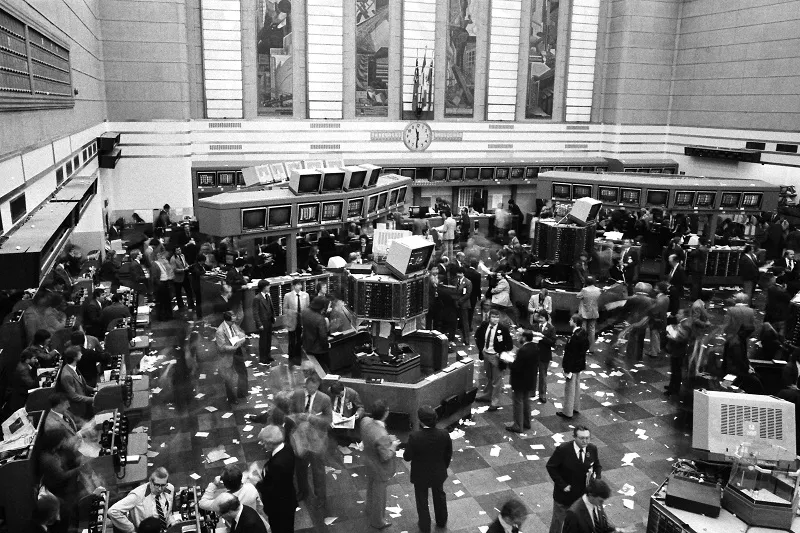
\includegraphics[width=\textwidth,height=5.5cm,keepaspectratio,
%     trim=0 150 0 150,clip]{tse-1981.png}
%   \caption{Toronto Stock Exchange, Toronto, 1981}
%   \Description{A panoramic view of the Toronto Stock Exchange 
%     building in 1981.}
%   \label{fig:teaser}
% \end{teaserfigure}


\maketitle

\section{Introduction}
  Synthetic market data generation has become an important tool in
  finance, particularly for time series such as asset returns, trading
  volume, and limit order books \cite{Potluru24, Horvath2025}. It can
  help researchers simulate fat-tail behavior, volatility clustering,
  and back-testing scenarios for prediction and hedging algorithms
  \cite{Stenger24}.

  Despite this growth, evaluation practices remain poorly
  standardized. Stenger et al. surveyed 56 studies and found little
  consensus on the metrics used or how they should be interpreted
  \cite{Stenger24}. As a result, comparisons across methods are often
  difficult and their relative strengths remain unclear.

  \subsection{A Brief Overview on Market Generators}
    Synthetic market data are multivariate time series related to
    financial assets and market microstructures, such as limit order
    books, trading volume, volatility surfaces, and asset returns
    \cite{Assefa2019, Stenger24, Horvath2025}. Researchers and
    practitioners are mainly interested in them for two reasons
    \cite{Horvath2025}: forecasting and prediction, where synthetic
    paths can support model training and evaluation, and simulating
    market scenarios, where they can reproduce rare events and
    stress-test strategies. Recent generative models such as GANs and
    VAEs, especially conditional variants, are attractive because they
    can learn conditional distributions of financial time series rather
    than only point estimators \cite{Horvath2025}.

  \subsection{Limitations in Market Generator Literature}
    Existing evaluation practices for synthetic time series remain
    fragmented, with no broadly accepted standard \cite{Wang20,
    Stenger24}. Many measures are poorly defined, inconsistently
    implemented, and hard to reproduce \cite{Stenger24}. This is
    especially problematic for generative tasks, where evaluation must
    capture more than marginal similarity and instead reflect temporal
    structure, diversity, and downstream utility \cite{Stenger24,
    Horvath2025}. Our review highlights four main limitations:

    \begin{enumerate}[label=\textbf{[L\arabic*]}]
      \item \label{limitation:metrics}
        \textbf{Inconsistent evaluation metrics:} Different studies use
        different measures, making comparisons difficult
        \cite{Stenger24}.

      \item \textbf{Lack of standardized datasets and preprocessing:}
        Benchmarking is often done on different assets, horizons, and
        preprocessing choices, which weakens comparability
        \cite{Stenger24}.

      \item \textbf{Narrow evaluation scope:} Many studies focus on
        marginal distributions and overlook temporal dependencies,
        diversity, and downstream usefulness \cite{Stenger24,
        Horvath2025}.

      \item \textbf{Reproducibility issues:} Missing implementations and
        detailed protocols make results hard to verify across studies
        \cite{Stenger24, Potluru24}.
    \end{enumerate}

  \subsection{Our Contributions}
    We develop a unified benchmark for synthetic equity-return
    generation that combines statistical and utility-based evaluation.
    Building on the taxonomy of Stenger et al. \cite{Stenger24}, the
    framework of Ang et al. \cite{Ang23}, and utility-focused work by
    Boursin et al. and Fecamp et al. \cite{Boursin22, Fecamp20}, we
    study how different metrics trade off in practice. Our key
    contributions are:

    \begin{enumerate}[label=\textbf{[C\arabic*]}]
      \item \label{contribute:1} \textbf{A consolidated evaluation
        framework:} We review and integrate measures from prior work
        to provide a more systematic benchmark for market generators
        \cite{Stenger24, Ang23, Boursin22}.

      \item \label{contribute:2} \textbf{Unified statistical and utility
        measures:} We combine fidelity metrics with downstream utility
        metrics in a single evaluation suite.

      \item \label{contribute:3} \textbf{An open benchmark framework:}
        We provide an open-source setup to support more consistent
        comparisons in future market-generator research.
    \end{enumerate}

  \subsection{Research Questions}
    Our benchmark addresses three main questions:
    \begin{enumerate}[label=\textbf{[Q\arabic*]}]
      \item How do different training sequence lengths affect generator
        performance?
      \item Are there trade-offs between fidelity, diversity, and
        downstream utility?
      \item Do modern deep-learning generators outperform classical
        parametric models in practical tasks?
    \end{enumerate}
    These questions are explored further in
    §\ref{sec:generator-framework} and the evaluation sections that
    follow.


\section{Preliminaries}
  \subsection{Problem Definition}\label{prelim:definition}
    Let us formally define the market generation problem. Given a
    financial time series of asset price movements
    $\mathbf{X} = (\mathbf{X}_1,\ldots,\mathbf{X}_I)^T = (\mathbf{X}_t)_{t=1}^T\in \mathbb R^{T\times I}$
    with $I$ individual securities spanning time $T$, let $p(\mathbf{X})$ denote
    its real distribution. The objective of the market generator is to
    synthesize a time series $\hat{\mathbf{X}} = (\hat{\mathbf{X}}_t)_{t=1}^T$
    such that its distribution $q(\hat{\mathbf{X}})$ approximates $p(\mathbf{X})$ while
    preserving key stylized facts, generating diverse samples, and
    improving downstream task training and evaluation. More importantly
    we wish to evaluate the generalization capabilites of $q(\hat{\mathbf{X}})$
    against unseen data $p(\mathbf{X}_{\mathrm{new}})$.

  \subsection{Scope of Project}
    \subsubsection{Evaluated Methods}
      Our benchmark covers models from classical parametric methods to
      modern deep-learning architectures. We selected models that meet
      one of three criteria: (1) proven industry adoption, (2) research
      community acceptance, and (3) recent methodological innovation.

      Classical parametric models rely on predefined statistical
      distributions and assumptions about the data-generating process.
      They remain common in financial institutions because of their
      interpretability and strong theoretical foundations.

      We also evaluate modern deep-learning approaches, especially
      models that learn the data distribution directly from
      observations rather than assuming a specific form. These include
      generative adversarial networks and variational autoencoders,
      which represent the current state of the art in synthetic market
      data generation.

      An overview of the market-generator classes is provided in
      §\ref{sec:model-overview}.

    \subsubsection{Datasets}
      The benchmark aims to generate realistic and diverse synthetic
      time series from daily financial asset prices over 15 years
      (2010--2025), collected from Yahoo Finance. To evaluate
      cross-asset behavior, we include 20 US large-cap stocks from
      several sectors and 5 popular US index-tracking ETFs (see table
      \ref{tab:asset-classification})

        \begin{table}[t]
        \centering
        \caption{Asset classification used in StonkBench.}
        \label{tab:asset-classification}
        \begin{tabular}{l l l l}
        \hline
        Ticker & Name & Type & Sector/Exposure \\
        \hline

        AAPL & Apple & Stock & Technology \\
        MSFT & Microsoft & Stock & Technology \\
        NVDA & NVIDIA & Stock & Technology \\
        AVGO & Broadcom & Stock & Technology \\
        JPM & JPMorgan Chase & Stock & Financials \\
        LLY & Eli Lilly & Stock & Healthcare \\
        UNH & UnitedHealth Group & Stock & Healthcare \\
        AMZN & Amazon & Stock & Consumer Disc. \\
        TSLA & Tesla & Stock & Consumer Disc. \\
        CAT & Caterpillar & Stock & Industrials \\
        UNP & Union Pacific & Stock & Industrials \\
        META & Meta Platforms & Stock & Communication \\
        NFLX & Netflix & Stock & Communication \\
        PG & Procter \& Gamble & Stock & Consumer Staples \\
        COST & Costco Wholesale & Stock & Consumer Staples \\
        XOM & Exxon Mobil & Stock & Energy \\
        CVX & Chevron & Stock & Energy \\
        NEE & NextEra Energy & Stock & Utilities \\
        PLD & Prologis & Stock & Real Estate \\
        LIN & Linde & Stock & Materials \\
        SPY & S\&P 500& ETF & S\&P 500 \\
        QQQ & Nasdaq-100& ETF & Nasdaq-100 \\
        XLF & Finance & ETF & U.S. Financials \\
        IWM & Russell 2000& ETF & Small Caps \\
        XLV & Health Care & ETF & U.S. Healthcare \\
        \hline
        \end{tabular}
    \end{table}

    \subsubsection{Scope of Evaluation Taxonomical Criteria}
      Our evaluation framework follows the taxonomy proposed by
      Stenger et al. \cite{Stenger24} and incorporates measures from
      multiple papers in the field.

      We integrate evaluation metrics from several sources while
      maintaining a structured taxonomy, providing broad coverage of
      the key aspects of evaluation and setting a standard for future
      market-generator research. A full description of the evaluation
      suite is provided in §\ref{subsec:stats-measure} and
      §\ref{sec:utility}.

\section{Overview of Market Generator Methods}
\label{sec:model-overview}
  We categorize synthetic financial time series generation methods into
  two main families: classical stochastic (parametric) models, which
  rely on explicit assumptions about the data-generating process, and
  modern deep learning (deep learning) models, which learn complex
  dependencies directly from data without predefined functional forms.
  The following subsections provide a detailed overview of the methods
  included in our benchmark.


  \subsection{Classical Stochastic (Parametric) Methods}
  \label{sub:parametric-methods}
    Parametric models assume a specific functional form for the 
    data generating process, characterised by a finite set of 
    parameters. These models are interpretable and analytically 
    tractable, allowing for closed-form solutions in many cases. 
    However, they may struggle to capture complex stylised facts 
    or high-dimensional dependencies beyond their structural 
    assumptions. Below we outline several widely-used parametric 
    models in financial markets.\\

      \begin{table}[h]
        \centering
        \caption{Common notation and variables.}
        \label{tab:notation}
        \begin{tabular}{ll}
        \toprule
        \textbf{Symbol} & \textbf{Description} \\
        \midrule
        \( S_t \) & Asset price \\
        \( X_t = \ln S_t \) & Log-price \\
        \( r_t = \ln(S_t / S_{t-1}) \) & Log-return \\
        \( \mu \) & Drift \\
        \( \sigma \) & Volatility \\
        \( W_t \) & Standard Brownian motion \\
        \( \Delta t \) & Discrete time step \\
        \bottomrule
        \end{tabular}
      \end{table}
        
        

      \begin{enumerate}[label=\textbf{[A\arabic*]}]
        \item \label{alg:gbm} \textbf{Geometric Brownian Motion 
        (GBM).} 
        The price process follows a continuous-time stochastic 
        process with constant drift and volatility. Model-specific 
        parameters are \(\mu\) and \(\sigma\).
        \begin{equation}
        dS_t = \mu S_t\,dt + \sigma S_t\,dW_t.
        \label{eq:gbm}
        \end{equation}

        \item \label{alg:ou} \textbf{Ornstein–Uhlenbeck (OU).} 
        A mean-reverting Gaussian process for log-prices or 
        spreads. Model-specific parameters are \(\theta>0\) 
        (reversion rate), \(\mu\) (long-term mean), and \(\sigma\) 
        (volatility).
        \begin{equation}
        dX_t = \theta(\mu - X_t)\,dt + \sigma\,dW_t.
        \end{equation}

        \item \label{alg:mjd} \textbf{Merton Jump Diffusion (MJD).} 
        Extends the GBM equation \eqref{eq:gbm} by incorporating 
        normally-distributed jumps. 
        Model-specific parameters are \(\lambda\) (jump intensity), 
        \(\mu_j\) and \(\sigma_j\) (mean and standard deviation of 
        jump sizes).
        \begin{equation}
        \frac{dS_t}{S_t} = \mu\,dt + \sigma\,dW_t + J\,dN_t,\\
        \end{equation}
        where $J \sim \mathcal N(\mu_j, \sigma_j^2),\quad N_t\sim\mathrm{Poisson}(\lambda t)$.


        \item \label{alg:dejd} \textbf{Double-Exponential Jump 
        Diffusion (DEJD).} 
        Another jump-diffusion model with asymmetric double-exponential 
        jump sizes modifying equation \eqref{eq:gbm}. 
        Model-specific parameters are \(p\) 
        (probability of upward jump) and \(\eta_1, \eta_2\) 
        (exponential parameters for upward/downward jumps).
        \begin{align}
          \frac{dS_t}{S_t} &= \mu\,dt + \sigma\,dW_t + Y\,dN_t,\\
          Y &=
          \begin{cases}
          \mathrm{Exp}(\eta_1), &\text{with probability } p,\\[4pt]
          -\mathrm{Exp}(\eta_2), &\text{with probability } 1-p.
          \end{cases} \nonumber
        \end{align}

        \item \label{alg:garch} \textbf{GARCH(1,1).} 
        A discrete-time conditional heteroskedastic model for 
        returns. Model-specific parameters are \(\omega>0,\ 
        \alpha\ge0,\ \beta\ge0\) (GARCH coefficients) and 
        \(\mathcal D\) (innovation distribution, usually standard 
        Normal or Student-t). Captures volatility clustering via 
        time-varying conditional variance.
        \begin{align}
          r_t &= \sigma_t z_t,\quad z_t\sim\mathcal D,\\
          \sigma_t^2 &= \omega + \alpha r_{t-1}^2 + \beta \sigma_{t-1}^2. \nonumber
        \end{align}
      \end{enumerate}


  \subsection{Deep Learning Methods}\label{sub:deep-learning-methods}
    Deep learning models, in this context, refer to generative 
    (often implicit) models that do not assume a fixed parametric 
    form for the underlying data-generating process. Instead, they 
    learn latent structures directly from data through flexible 
    architectures such as neural networks, enabling the modeling 
    of highly nonlinear, high-dimensional, and multi-modal 
    dependencies (e.g., multivariate financial time series with 
    interactions across assets, time horizons, and features). 
    While these models trade off interpretability and analytical 
    tractability, they offer substantially greater expressive 
    power and flexibility. This expressiveness, however, comes at 
    the cost of increased data requirements, more intensive 
    hyperparameter tuning, and higher computational demands. 

    We categorize these approaches into two major families of
    deep generative models, considered in this paper: 
    Generative Adversarial Networks (GANs)
    and Variational Autoencoders (VAEs).
    

  %   \subsubsection{Diffusion Models}
  %     Diffusion models (or score-based generative models) have 
  %     emerged as powerful methods for modeling complex data 
  %     distributions via a forward (noise-adding) process and a 
  %     learned reverse (denoising) process \cite{ho2020denoising}. 
  %     In the forward direction, one gradually corrupts a data sample 
  %     \(x_0\) into noise via a Markov chain:
  %    
  %     \begin{align}
  %       q(x_{1:T}\mid x_0) &= \prod_{t=1}^T q(x_t \mid x_{t-1}), \\
  %       q(x_t \mid x_{t-1}) &= \mathcal{N}\left(x_t; \sqrt{1-\beta_t}\,x_{t-1}, \beta_t I\right). \nonumber
  %     \end{align}
  %    
  %     
  %     The reverse (generative) model is parameterized as
  %     \[
  %       p_\theta(x_{t-1} \mid x_t) = \mathcal{N}\bigl(x_{t-1}; 
  %       \mu_\theta(x_t, t), \Sigma_\theta(x_t, t)\bigr),
  %     \]
  %     where \(\mu_\theta\) and \(\Sigma_\theta\) are often 
  %     expressed via a neural network that estimates the score 
  %     \(\nabla_{\theta} \log p_\theta(x_t)\). A common training 
  %     objective is the simplified denoising score-matching loss:
  %     \[
  %       \mathbb{E}_{t, x_0, \epsilon}\Bigl[ \bigl\| \epsilon - \epsilon_\theta(x_t, t)\bigr\|^2 \Bigr],
  %     \]
  %     where \(x_t = \sqrt{\bar\alpha_t}\,x_0 + \sqrt{1-\bar\alpha_t}\,\epsilon\).
  %     
  %     In finance/time-series, diffusion models have recently been 
  %     adapted to generate synthetic asset paths by converting 
  %     multivariate time series into suitable representations (e.g. 
  %     wavelet-transformed images) and then sampling via reverse 
  %     diffusion \cite{Tanaka25}. For instance, Takahashi and Mizuno 
  %     shows that such an approach can reproduce key statistical 
  %     properties of financial data (e.g.\ volatility clustering, 
  %     tail behavior) \cite{Takahashi24}.  
  %     Another relevant work is "A Financial Time Series Denoiser 
  %     Based on Diffusion Model", which shows how diffusion can help 
  %     improve downstream predictability and reduce noise in 
  %     financial signals \cite{wang24denoiser}.
    \subsubsection{Variational Autoencoders (VAEs)}
    VAEs \cite{kingma2022vae, 
    rezende2014stochastic} are latent-variable generative models 
    that posit a probabilistic encoder \(q_\phi(z \mid x)\) and 
    decoder \(p_\theta(x \mid z)\). One maximizes the evidence 
    lower bound (ELBO):
    \[
    \mathcal{L}_{\text{VAE}} = \mathbb{E}_{q_\phi(z \mid x)}
    \bigl[\log p_\theta(x \mid z)\bigr] - \mathrm{KL}\bigl(
    q_\phi(z \mid x)\,\Vert\,p(z)\bigr).
    \]
    Often one uses a standard Gaussian prior \(p(z) = 
    \mathcal{N}(0, I)\). The encoder–decoder structure allows 
    sampling by first drawing \(z \sim p(z)\), then generating 
    \(x \sim p_\theta(x \mid z)\).
    
    In financial time-series generation, specialized versions such 
    as the Time-Causal VAE (TC-VAE) have been proposed to enforce 
    causality in the encoding/decoding of temporal data. For 
    instance, Acciaio et al.\ (2024) propose TC-VAE, which 
    ensures that generated paths respect temporal causality and 
    show that the model reproduces stylized facts (e.g., heavy 
    tails, volatility clustering) on real markets 
    \cite{acciaio2024vae}. Because VAEs provide a principled 
    latent representation, they are useful in finance to model 
    underlying latent drivers of asset dynamics and to sample 
    coherent trajectories.
    \begin{enumerate}[label=\textbf{[A\arabic*]},resume]
      \item \label{alg:timevae} \textbf{TimeVAE.}
      A time-series specific VAE variant that combines causal
      temporal encoders (e.g., causal convolutions or RNNs) with an
      autoregressive decoder to preserve path coherence. Training
      typically augments the ELBO with prediction or stepwise
      reconstruction losses to improve short- and long-range
      dependencies; TimeVAE is used in our benchmark as a
      dedicated VAE baseline for temporal data \cite{Desai21}.
    \end{enumerate}
    
    \subsubsection{Generative Adversarial Networks (GANs)}
    GANs models approach 
    generation as a two-player game between a generator \(G\) and 
    a discriminator \(D\) \cite{Goodfellow14}. The discriminator 
    is trained to 
    maximize the probability of correctly classifying real data 
    and generated data, with loss
    \[
    L_D = -\mathbb{E}_{x \sim p_{\text{data}}}\bigl[\log D(x)
    \bigr] - \mathbb{E}_{z \sim p(z)}\bigl[\log (1 - D(G(z)))
    \bigr].
    \]
    The generator aims to fool the discriminator and is trained to 
    minimize
    \[
    L_G = -\mathbb{E}_{z \sim p(z)}[\log D(G(z))].
    \]
    Many GAN variants, such as Wasserstein GAN or Least Squares 
    GAN, modify these loss functions to promote more stable 
    training and address issues like mode collapse \cite{Goodfellow14} .
    
    In financial data synthesis, GANs have been widely used to 
    generate realistic synthetic time series. For example, 
    GAN-based financial data generation models (often using WGAN 
    or improvements) show that one can improve the authenticity 
    and predictive ability of generated financial statements or 
    time series \cite{Qi25}. Another example is 
    VRNNGAN, which uses a recurrent VAE as the generator and a 
    recurrent discriminator to capture temporal dependencies in 
    synthetic sequence generation \cite{Lee22}. GANs are 
    relevant in finance because they can capture complex joint 
    distributions and dependencies in multivariate time-series 
    without requiring explicit likelihood models.
    
    \begin{enumerate}[label=\textbf{[A\arabic*]},resume]
      \item \label{alg:quantgan} \textbf{QuantGAN.}
      A GAN variant tailored for financial applications that
      incorporates quantile-aware objectives or conditional
      quantile matching and temporal architectures (e.g.,
      temporal convnets or transformers). QuantGANs aim to better
      capture tail behaviour and risk-sensitive statistics
      (e.g., VaR/CVaR) important for downstream financial tasks
      \cite{Wiese2020}.
    \end{enumerate}
  \subsection{Non-parametric}
  Non-parametric models are generator classes that does not rely
  on probability distribution assumptions or, in the case of Bayesian
  non-parametric models, does not require a specified model parameters.
  Among the simplest but most effective of the non-parametric models are
  the variations of time series block boostrap that, in general, sample
  blocks of time data to preserve temporal dependencies.
  \ref{sub:deep-learning-methods}.
  \begin{enumerate}[label=\textbf{[A\arabic*]}, resume]
        \item \label{alg:blockbootstrap2} \textbf{Block Bootstrap 
        (Resampling Method).} 
        A resampling technique that preserves short-range 
        dependence by sampling contiguous blocks of returns. 
        Although not parametric, it is included here for 
        completeness and baseline comparison.
      \end{enumerate}

      \begin{figure*}[h]
        \centering
        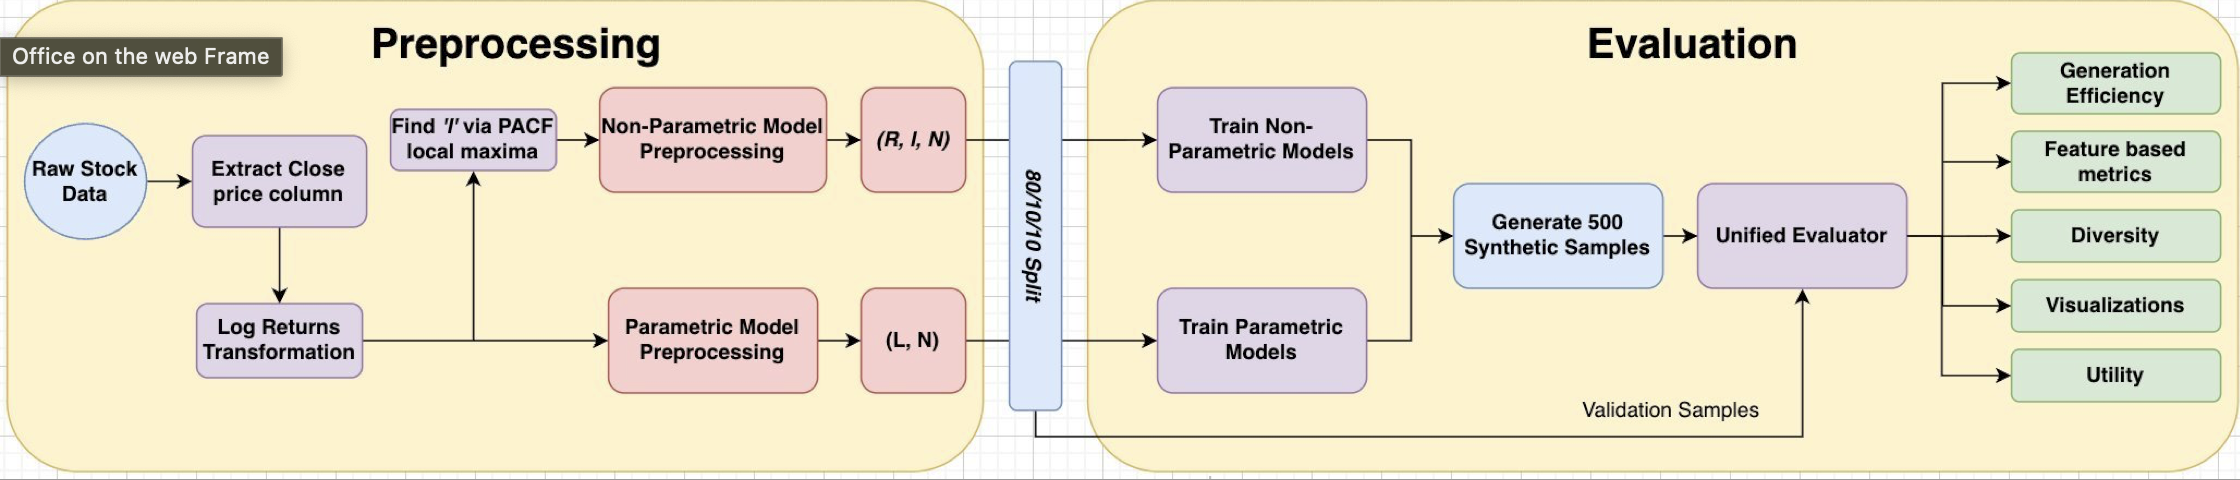
\includegraphics[width=\textwidth,keepaspectratio]{../../results/stonk_bench_architecture.png}
        \caption{Stonk Bench system architecture overview.}
        \Description{Diagram illustrating the complete Stonk Bench pipeline including data preprocessing, model evaluation, and benchmark framework components.}
        \label{fig:stonk_bench_architecture}
      \end{figure*}



\section{Market Generator Framework}\label{sec:generator-framework}
It is important to have standardized generation framework as
part of our efforts to create a unified benchmark \ref{contribute:3};
this section outines the details of the dataset used, preprocessing, and
 generation framework used by StonkBench for models to train on 
 historical market data.

\subsection{Data preprocessing}\label{subsec:data-preprocess}
    \subsubsection{Dataset Split}
    Given our stock price dataset, we perform a chronological
    ten-two-three year partition into training, validation, and testing
    datasets from 2010 to 2025, where $D = D^{\mathrm{train}}, D^{\mathrm{val}}, D^{\mathrm{test}}$ denotes the concatenation.
    This deviates from the training scheme proposed by TSGBench \cite{Ang23}; we wish to 
    hold out our testing time-horizon from the training set completely
    to evaluate model generalization capabilities.
    
    \subsubsection{Log Return Transformation}
    We then transform the price time series for both sets into a log return time series, 
    which is a common practice in financial modeling to stabilize variance 
    and make the data more suitable for analysis. The return \( \mathbf{R}_t \) at time \( t \) is calculated as
    \footnote{The log return operation is applied channel-wise to the time series.}
    \footnote{From now, on we refer to $D$ as the log return time series dataset and notate it as $\mathbf{R}_t$
    to avoid notation clutering, unless explicitly stated otherwise.}:
    \begin{equation}
    \mathbf{R}_t := \log\left(\frac{\mathbf{S}_t}{\mathbf{S}_{t-1}}\right) = \log(\mathbf{S}_t) - \log(\mathbf{S}_{t-1}),
    \end{equation}

    \subsubsection{Sliding Window Transformation}
    The deep learning models considered in §\ref{sub:deep-learning-methods} require a fixed-length data
    for training and generation. Therefore, to standardize input and data generation, while preserving temporal dependencies,
    we apply a sliding window transformation to the log return time series. Given a
    window length $L\in\mathbb{N}$, we applying a sliding window operation $W_L$ over the time
    series as follows.
    \begin{equation}
        W_L: (\mathbf{R}_t)_{t=1}^T \mapsto \{ \mathbf{w}_t \coloneq(\mathbf{R}_t,\mathbf{R}_{t+1},\dots, \mathbf{R}_{t+L}): 1\leq t \leq T-L\}
    \end{equation}
    We denote the resulting set of windows, for a given data partition from $D$, as $\mathcal{D}^i\coloneq W_L(D^i)$ for $i\in\{\mathrm{train}, \mathrm{val}, \mathrm{test}\}$.
    For the purpose of research, we expirment our generation training with windown lenghts $L\in\{ 21, 63, 126 ,252\}$ , represeneting
    general the number of trading days in a month, a quarter, half a year and a year, respectively
    
    \footnote{TSGBench determined the window length for deep learning training 
    and generation depending on the dataset by finding the maximum auto-correlation of that time
    series dataset \cite{Ang23}}.


\subsection{Market Generator Training and Generation}\label{subsec:generator-training}
    We train each market generator on the log-return training data to
    produce synthetic windows, each with shape $L\times I$. Formally,
    for each generator $G_g$, $g\in\mathcal{G}$, we generate $N$ synthetic
    windows and obtain the generated set
    $\hat{\mathcal{D}}_g = \{\hat{\mathbf{w}}_n: \hat{\mathbf{w}}_n \sim G_g(\mathbf{w} \mid D^{\mathrm{train}})\}_{n=1}^N$.
    Here, $\mathcal{G}$ is the index set of market generators considered in
    §\ref{sec:model-overview}, $\hat{\mathbf{w}}_n$ denotes a synthetic
    window of size $L\times I$, and $N$ is the number of synthetic windows
    generated for each model, which we set to $N=1000$.

    \subsubsection{Non-deep Learning Model Generation}
    Parametric and bootstrap generators are fit on $D^{\mathrm{train}}$ and then
    sample windows directly from the learned process or resampled data.
    \begin{align}
        \hat{\mathbf{S}}_{n_l} \sim G_g(\mathbf{S} \mid D^{\mathrm{train}}), \quad
        \hat{\mathbf{w}}_n \coloneq (\hat{\mathbf{S}}_{n_1},\dots, \hat{\mathbf{S}}_{n_L}), \quad
        \hat{\mathcal{D}}_g = \{\hat{\mathbf{w}}_n\}_{n=1}^N.
    \end{align}

    \subsubsection{Deep Learning Model Generation}
    Deep-learning frameworks in this paper (GAN, VAE, DDPM, and
    signature-based models) are trained on the sliding-window transform
    $W_L(D^{\mathrm{train}})$ (see §\ref{subsec:data-preprocess}). They then
    generate $N$ independent windows of size $L$, each with shape
    $L\times I$, directly from the learned window distribution:
    \begin{align}
        \hat{\mathbf{w}}_n \sim G_g(\mathbf{w} \mid W_LD^{\mathrm{train}}), \qquad
        \hat{\mathcal{D}}_g = \{\hat{\mathbf{w}}_n\}_{n=1}^N.
    \end{align}












  \section{Statistical Evaluation Measures}\label{sec:stat-eval}
    The statistical metrics considered in this paper are used to
    evaluate either the realism of synthetic market data to its
    trained history or generative novelty in market scenarios.
    The following subsections describes the metrics considered and
    the evaluatiom framework applied.
    
    \subsection{Statistical Measures}\label{subsec:stats-measure}
    As described in \ref{limitation:metrics}, our contribution 
    \ref{contribute:1} is based on a well-established taxonomy framework
    \cite{Stenger24} while introducing our industry-specific stylized
    facts to holistically evaluate the characteristics of synthetic
    market data. We divide our statistical metrics
    \subsubsection{Fidelity Measures}
    These metrics quantify how well synthetic data captures key 
    marginal and second-order properties of real data. We employ
    the following feature-based metrics:

      \begin{enumerate}[label=\textbf{[M\arabic*]}]
        \item \label{metric:mdd} \textbf{Marginal Distribution 
        Difference (MDD):}  
        To measure the distance between empirical marginal distributions
        of real versus synthetic data, we use the 1-Wasserstein distance
        (a.k.a. Earth Mover's distance). This was chosen over the 
        popular Kullback-Leibler divergence or the derivatives
        Jensen-Shannon divergence due to its better numerical stability
        and ability to capture distributional differences even when
        supports do not overlap \cite{Arjovsky17}.
        \[
        \begin{aligned}
          \mathrm{MDD} &= W_1\big(\widehat{F}_{\text{real}}, 
          \widehat{F}_{\text{synth}}\big), \\
          W_1(F, G) &= \int_0^1 \big|F^{-1}(u) - G^{-1}(u)\big|\,du,
          \end{aligned}
          \]
          where \(\widehat{F}_{\text{real}}\) and \(\widehat{F}_{\text{synth}}\) 
          are empirical CDFs.
          
          \end{enumerate}
          The following four metrics capture differences in the first four
          statistical (central) moments between real and synthetic data.
          \begin{enumerate}[label=\textbf{[M\arabic*]}, resume]
          
          \item \label{metric:md} \textbf{Mean Difference (MD):}  
          \[
          \mathrm{MD} = \big|\mu_{\text{real}} - \mu_{\text{synth}}\big|.
          \]
          
          \item \label{metric:sdd} \textbf{Standard Deviation Difference (SDD):}  
          \[
          \mathrm{SDD} = \big|\sigma_{\text{real}} - \sigma_{\text{synth}}\big|.
          \]

          \item \label{metric:skewness} \textbf{Skewness Difference (SD):}  
          \begin{align*}
          \mathrm{SD} =& \big|\gamma(r_{\text{real}}) - \gamma(r_{\text{synth}})\big|, \\
          \gamma(r) =& \frac{\mathbb{E}[(r - \mu)^3]}{(\sigma)^3}.
          \end{align*}
          
          \item \label{metric:kd} \textbf{Kurtosis Difference (KD):}  
          \begin{align*}
          \mathrm{KD} &= \big|\kappa^{\mathrm{ex}}(r_{\text{real}}) 
          - \kappa^{\mathrm{ex}}(r_{\text{synth}})\big|, \\
          \kappa^{\mathrm{ex}}(r) &= \frac{\mathbb{E}[(r - \mu)^4]}{(\sigma)^4} - 3.
          \end{align*}
          
          \end{enumerate}
          
          \subsubsection{Visualization Methods} \label{sec:visualization_methods}
          Visual tools complement numeric metrics for face-validity and 
          communication \cite{Ang23}.
          \begin{enumerate}[label=\textbf{[M\arabic*]}, resume]
          \item \label{metric:tsne} \textbf{t-SNE:}  
          2D embeddings of window-level features for real 
          versus synthetic overlap and cluster structure.
          
          \item \label{metric:dist} \textbf{Distribution:}  
          Histograms of returns to visualize empirical 
          distribution.
          \end{enumerate}
          
          \subsubsection{Diversity Measures}
          We are also interested if the SDGFTS can generate data
          not observed but follow the same distribution as the real data.
          Therefore, we include the following intra-class distance
          metrics. The inclusion of
          these metrics are chose to ensure that mode collapse 
          is prevented. 

          
          \begin{enumerate}[label=\textbf{[M\arabic*]}, resume]
          \item \label{metric:ed} \textbf{Intra-Class Euclidean 
          Distance (ICD-ED):}  
          \[
          \mathrm{ICD\text{-}ED} = \frac{2}{R(R-1)} 
          \sum_{1 \le a < b \le R} \left\| \textbf{r}_a - 
          \textbf{r}_b \right\|_2,
          \]
          where \(\textbf{r}_a \in \mathbb{R}^{L}\) is the \(a\)-th 
          sample.
          
          \item \label{metric:dtw} \textbf{Intra-Class Dynamic Time 
          Warping (ICD-DTW):}  
          \[
          \mathrm{ICD\text{-}DTW} = \frac{2}{R(R-1)} 
          \sum_{1 \le a < b \le R} d_{\mathrm{DTW}}\bigl(
          \textbf{r}_a, \textbf{r}_b\bigr).
          \]
          \end{enumerate}
          
          \subsubsection{Efficiency Measures}
          Generation efficiency is crucial for practical applications,
          especially in high-frequency trading or real-time risk
          management, where rapid data synthesis is required.
          Thus, we include the following efficiency metric \cite{Stenger24}.
          \begin{enumerate}[label=\textbf{[M\arabic*]}, resume]
          \item \label{metric:gentime} \textbf{Generation Time:}  
          Wall-clock time to generate \(S\) samples:
          \[
          T_{\mathrm{gen}} = t_1 - t_0 \quad (\text{seconds for } 1,000
          \text{ samples}).
          \]
          \end{enumerate}
          
          \subsubsection{Stylized Facts Measures} \label{sec:stylized-facts}
          Canonical stylized facts:
          
          \begin{enumerate}[label=\textbf{[M\arabic*]}, resume]

          \item \label{metric:acd} \textbf{Autocorrelation Difference 
          (ACD):}  
          Absolute difference in lag-1 autocorrelation:
          \[
          \begin{aligned}
          \rho(1) &= \frac{\sum_{t=2}^{L} (r_t - \bar{r})
          (r_{t-1} - \bar{r})}
               {\sum_{t=1}^{L} (r_t - \bar{r})^2}, \\
          \mathrm{ACD} &= \big|\rho_{\text{real}}(1) - 
          \rho_{\text{synth}}(1)\big|.
          \end{aligned}
          \]
          
          \item \label{metric:volclustering} \textbf{Volatility 
          Clustering (VC):}  
          Lag-1 autocorrelation of squared or absolute returns measures 
          volatility clustering, a stylized fact where large price movements 
          tend to cluster in time \cite{Cont01}:
          \[
          \begin{aligned}
          \rho_{r^2}(1) &= \mathrm{Corr}\big((r_t)^2, 
          (r_{t-1})^2\big), \\
          \rho_{|r|}(1) &= \mathrm{Corr}\big(|r_t|, 
          |r_{t-1}|\big).
          \end{aligned}
          \]

        \item \label{metric:slow_decay} \textbf{Long Memory / Slow Decay (LMSD):}  
        To quantify long-range dependence in volatility, we follow
        Cont (2001) \cite{Cont01} and study the autocorrelation of
        absolute (or squared) returns:
        \[
        C_\alpha(\tau) \,=\, \mathrm{corr}\!\big(|r_{t+\tau}|^\alpha,\,
        |r_t|^\alpha\big), \qquad \alpha \in \{1,2\}.
        \]
        Empirically, this correlation decays slowly according to a
        power law,
        \[
        C_\alpha(\tau) \,\sim\, \frac{A}{\tau^{\beta}}, \qquad
        \beta \in [0.2,\,0.4],
        \]
        indicating persistent volatility fluctuations (long memory).
        For evaluation, we estimate the decay exponent by a
        log--log linear fit over lags 
        \(\tau \in \{1,\ldots, \tau_{\max}\}\) where
        \(C_\alpha(\tau) > 0\):
        \[
        \widehat{\beta} \,=\, -\,\text{slope}\Big(\log C_\alpha(\tau)
        \;\text{vs.}\; \log \tau\Big).
        \]
        Our metric is the absolute difference between decay exponents
        estimated on real and synthetic data:
        \[
        \mathrm{LMSD} \,=\, \big|\widehat{\beta}_{\text{real}} -
        \widehat{\beta}_{\text{synth}}\big|.
        \]
        Unless otherwise stated, we set \(\alpha=1\) (absolute returns)
        and report \(\widehat{\beta}\) together with the goodness-of-fit
        of the linear regression.
        \end{enumerate}
    
    \subsection{Statistical Evaluation Framework}
    We compare the statistical measures outlined above between the synthetic
    market data to the trained historical dataset. Consider a market generator
    $G_j, j\in\mathcal{J}$ trained on the dataset $D^{train}$ and its generated data
    $\mathcal{D}_{G_j}$ as specified in \ref{subsec:generator-training},
    we can apply an evaluation metric E, as mentioned in \ref{subsec:stats-measure}, defined an measurable function 
    $\mathbb{R}^{T\times K}\to \mathbb{R}$.
\section{Utility Evaluation of Downstream Tasks}\label{sec:utility}
Most market generator research focuses on statistical similarity while
overlooking practical downstream effects \cite{Horvath2025, Stenger24}.
While some work explores option hedging \cite{Tanaka25,Boursin22}, benchmarks
like TSGBench lack broader utility experiments. We introduce three
downstream tasks \ref{contribute:2} under a train-synthetic-test-real (TSTR)
framework \cite{Leznik21, Stenger24} --- option delta hedging (options
market maker), portfolio hedging (equity market maker), and alpha generation
(hedge fund manager) --- demonstrating synthetic data utility in realistic
settings \cite{Horvath2025}.

\subsection{Overview of Utility Evaluation}
    All three tasks follow a common protocol. Each task
    \(\mathcal{T}\) is specified by a loss function
    \(\mathcal{L}_{\mathcal{T}}\) over the model's policy \(\theta\), and
    the optimal policy is
    \begin{equation}
      \theta^{*} \coloneq \underset{\theta}{\arg\min}\;
      \mathcal{L}_{\mathcal{T}}(\theta),
      \label{eq:utility-optimal-policy}
    \end{equation}
    (or \(\arg\max\) for reward-type objectives). Policies are trained
    under the TSTR framework of §\ref{sec:utility-training-framework} on
    the data partition of §\ref{subsec:data-preprocess} with rolling-window
    validation for hyperparameter tuning \cite{Leznik21}, and scored with
    the metric toolbox of §\ref{sec:utility-evaluation}.

    \subsubsection{Utility Training and Evaluation Framework}
    \label{sec:utility-training-framework}
      Consider a market generator \(G_g\) with synthetic data
      \(\hat{\mathcal{D}}_g\). Training an algorithm \(A\) (e.g.\ a 5-layer
      perceptron) for task \(\mathcal{T}\) on
      \(\mathcal{D}^{\mathrm{train}}\) and \(\hat{\mathcal{D}}_g\) yields
      models \(M_r\) and \(\hat{M}_g\), respectively. Scoring both on the
      real test set \(\mathcal{D}^{\mathrm{test}}\) by a score \(S\)
      \footnote{WLOG, we assume a score on \(\mathbb{R}\) where higher is
      better} gives \(s_r\) and \(s_g\); the generator is useful for the
      pair \((\mathcal{T}, A)\) if \(s_g > s_r\), and the best generator is
      \(G_{g^{*}}\) with
      \(g^{*} \coloneq \max\{s_g : g \in \mathcal{G}\}\).

      \subsubsection{Augmented Training}
      \label{sec:augmented-training}
      We additionally train on the augmented set
      \(\tilde{\mathcal{D}}_j \coloneq \mathcal{D}^{\mathrm{train}} \cup
      \hat{\mathcal{D}}_j\), yielding \(\tilde{M}_j\), to assess whether
      synthetic data adds value on top of real training data.

    \subsubsection{Utility Evaluation Metrics}
    \label{sec:utility-evaluation}
      To make downstream evaluations comparable across tasks, we define a
      common toolbox of utility metrics used by researchers and
      practitioners. Given a downstream model \(M\) for task
      \(\mathcal{T}\), let \(\mathbf{\Pi}_M \coloneq (\pi_{t,i})_{t,i} \in
      \mathbb{R}^{L \times I}\) denote the trading portfolio generated by
      \(M\), where \(\pi_{t,i}\) is the trading order (position) in asset
      \(i\) at time \(t\). A utility metric \(U\) maps the portfolio to a
      scalar score \(u \coloneq U(\mathbf{\Pi}_M)\), instantiating the TSTR
      score \(S\) of §\ref{sec:utility-training-framework}, i.e.\
      \(s \equiv u = U(\mathbf{\Pi}_M)\) for
      \(M \in \{M_r, \hat{M}_j, \tilde{M}_j\}\). The per-period profit and
      loss (PnL) of the portfolio is
      \begin{equation}
        \mathrm{PnL}_t(\mathbf{\Pi}_M) \coloneq \sum_{i=1}^{I}
        \pi_{t,i}\, r_{t+1,i},
        \label{eq:utility-pnl}
      \end{equation}
      where \(r_{t+1,i}\) is the simple return of asset \(i\) over
      \([t, t+1)\). The toolbox evaluates the following metrics over the
      per-period PnL sequence
      \(\{\mathrm{PnL}_t(\mathbf{\Pi}_M)\}_{t=0}^{L-1}\):
      \begin{enumerate}[label=\textbf{[U\arabic*]}]
        \item \textbf{PnL.} Total profit and loss over the window,
        \(\mathrm{PnL}(\mathbf{\Pi}_M) \coloneq \sum_{t=0}^{L-1}
        \mathrm{PnL}_t(\mathbf{\Pi}_M)\).

        \item \textbf{Annualized Sharpe ratio.} The mean per-period PnL
        divided by its standard deviation,
        \begin{equation}
          \begin{split}
            \mathrm{Sharpe}(\mathbf{\Pi}_M) &\coloneq
            \frac{\hat{\mu}}{\hat{\sigma}}, \\\
            \hat{\mu} \coloneq \frac{1}{L}\sum_{t=0}^{L-1}
            \mathrm{PnL}_t, \quad &
            \hat{\sigma}^2 \coloneq \frac{1}{L-1}
            \sum_{t=0}^{L-1} \left(\mathrm{PnL}_t -
            \hat{\mu}\right)^2,
          \end{split}
          \label{eq:utility-sharpe}
        \end{equation}
        Since the evaluation horizon is a single trading year
        , no annualization factor (i.e.\ \(\sqrt{L}\))
        is applied.

        % \item \textbf{Entropic risk measure (ERM).} The risk-sensitive
        % certainty equivalent of the per-period PnL under exponential
        % utility with risk-aversion \(\gamma > 0\) \cite{Fecamp20},
        % \begin{equation}
        %   \mathrm{ERM}_\gamma(\mathbf{\Pi}_M) \coloneq
        %   -\frac{1}{\gamma}\log\frac{1}{L}\sum_{t=0}^{L-1}
        %   e^{-\gamma\, \mathrm{PnL}_t},
        %   \label{eq:utility-erm}
        % \end{equation}
        % which reduces to the mean PnL as \(\gamma \to 0\) and increasingly
        % penalizes losses as \(\gamma\) grows.

        \item \textbf{CVaR.} The conditional value at risk at level
        \(\alpha\), i.e.\ the expected loss in the worst \(\alpha\)-tail of
        the per-period PnL distribution \cite{Fecamp20},
        \begin{equation}
          \mathrm{CVaR}_\alpha(\mathbf{\Pi}_M) \coloneq
          -\mathbb{E}\left[\mathrm{PnL}_t \mid \mathrm{PnL}_t \leq
          \mathrm{VaR}_\alpha\right],
          \label{eq:utility-cvar}
        \end{equation}
        where \(\mathrm{VaR}_\alpha\) is the lower \(\alpha\)-quantile of
        the per-period PnL distribution.

        \item \textbf{Win rate.} The fraction of periods with positive
        PnL,
        \begin{equation}
          \mathrm{WR}(\mathbf{\Pi}_M) \coloneq \frac{1}{L}
          \sum_{t=0}^{L-1} \mathbb{I}\left\{\mathrm{PnL}_t >
          0\right\},
          \label{eq:utility-winrate}
        \end{equation}
        where \(\mathbb{I}\{\cdot\}\) is the indicator function.

        \item \textbf{Max drawdown.} The largest peak-to-trough decline
        of the cumulative PnL curve \(C_t \coloneq \sum_{s=0}^{t}
        \mathrm{PnL}_s\),
        \begin{equation}
          \mathrm{MDD}(\mathbf{\Pi}_M) \coloneq \max_{0 \leq u \leq v
          \leq L} \left(C_u - C_v\right).
          \label{eq:utility-mdd}
        \end{equation}
      \end{enumerate}

      Let \(u_n \coloneq U\left(\mathbf{\Pi}_M^{(n)}\right)\) be the value
      of a metric \(U\) on the \(n\)-th test window. We report each metric
      as
      \begin{equation}
          \bar{u} \coloneq \frac{1}{N}\sum_{n=1}^{N} u_n, \quad
          \hat{\sigma}_u \coloneq \sqrt{\frac{1}{N-1}
          \sum_{n=1}^{N} \left(u_n - \bar{u}\right)^2},
        \label{eq:utility-aggregation}
      \end{equation}
      the mean and standard deviation of \(U\) across all \(N \coloneq
      \vert\mathcal{D}^{\mathrm{test}}\vert\) test windows.

      Every task below instantiates the same protocol: train
      \(\{M_r, \hat{M}_j, \tilde{M}_j\}\) on
      \(\{\mathcal{D}^{\mathrm{train}}, \hat{\mathcal{D}}_j,
      \tilde{\mathcal{D}}_j\}\) per
      §\ref{sec:utility-training-framework}--\ref{sec:augmented-training},
      evaluate on \(\mathcal{D}^{\mathrm{test}}\), and report the toolbox
      metrics above.

\subsection{Option Delta Hedging}\label{sec:option-hedging}
    Option hedging is a popular downstream utility benchmark in market
    generator research \cite{Tanaka25, Boursin22}. We take the perspective
    of an options market maker selling a European call option on a cash
    equity to minimize counterparty risk when the call expires
    \cite{Fecamp20}.

    \subsubsection{Problem Definition}
    Consider a European call at strike \(K\), maturing at time \(L\), on
    cash equity \(i\) with payoff \(g(L) \coloneq (S_{L,i} - K)_+\),
    rebalanced at the discrete times \(\mathbb{T} \coloneq \{t \in
    \mathbb{N} : 0 \leq t \leq L-1\}\) (end-of-day). The hedger's policy
    is the hedge position \(\mathbf{\Delta} \coloneq (\Delta_t)_{t=0}^{L-1}
    \in \mathbb{R}^{L}\), i.e.\ the trading portfolio \(\mathbf{\Pi}_M
    \equiv \mathbf{\Delta}\). The loss is the quadratic replication
    error of the short call,
    \begin{equation}
      \mathcal{L}_{\Delta}(\mathbf{\Delta}) \coloneq
      \mathbb{E}\left[\left(g'(L) - \sum_{t=0}^{L-1} \Delta_{t}\,
      \tilde{g}(t)\, \left(e^{R_{t+1,i}} - 1\right)\right)^2\right],
      \label{eq:option-hedger-loss}
    \end{equation}
    where \(\tilde{g}(t) \coloneq S_{t,i}/K\) is the moneyness of the
    contract, \(\tilde{g}(L) \coloneq (S_{L,i}/K - 1)_+\) its payoff in
    moneyness units, and \(g'(L) \coloneq \tilde{g}(L) - c_0/K\) with
    \(c_0\) the call premium from the Black-Scholes-Merton equation. The
    optimal policy minimizes this loss,
    \begin{equation}
      \mathbf{\Delta}^{*} \coloneq \underset{\mathbf{\Delta}}{\arg\min}\;
      \mathcal{L}_{\Delta}(\mathbf{\Delta}).
      \label{eq:option-hedger-optimizer}
    \end{equation}

    \subsubsection{Framework}
    We use a long-short-term-memory (LSTM) network under the loss of
    equation \ref{eq:option-hedger-loss} \cite{Fecamp20}. While related
    work feeds raw price data \cite{Fecamp20,Boursin22,Tanaka25}, our
    framework recurrently feeds the moneyness \(\tilde{g}(t)\) instead of
    the raw price, allowing the network to generalize the payoff across
    strikes. At each step the LSTM takes the triplet
    \((\Delta_{t-1}, \tilde{g}(t), \tau_t)\) --- the previous hedge
    position, the current moneyness, and the normalized time-to-maturity
    \(\tau_t \coloneq 1 - t/L\).

    \subsubsection{Training}
    Since the LSTM hedges one asset at a time, each training window
    \(\mathbf{w} \in \mathcal{D}\) is treated as one channel. For each
    window we append an initial hedge \(\Delta(0) = 0\) and an initial
    moneyness \(\tilde{g}(0)\) \footnote{Equivalent to fixing the strike
    \(K = S_{0,i}/\tilde{g}(0)\) for the contract of maturity \(L\)},
    drawn from \(0.7\) to \(1.3\) at \(0.1\) increments \footnote{These
    values correspond to option contracts \(10\%\)--\(30\%\) out-of- and
    in-the-money relative to the initial price}, and propagate the
    log-moneyness recursively as
    \(\log \tilde{g}(t) = \log \tilde{g}(t-1) + R_{t,i}\)
    \footnote{For a training set of size \(N = \vert\mathcal{D}\vert\),
    this yields \(N \times 7\) training examples}. Models are trained per
    §\ref{sec:utility-training-framework}.

    \subsubsection{Evaluation}
    Models \(\{M_r, \hat{M}_j, \tilde{M}_j\}\) are scored on
    \(\mathcal{D}^{\mathrm{test}}\) with the toolbox of
    §\ref{sec:utility-evaluation}; we additionally report the hedging loss
    \(\mathcal{L}_{\Delta}\) of equation \ref{eq:option-hedger-loss},
    aggregated per equation \ref{eq:utility-aggregation}.

\subsection{Portfolio Hedging}
    Portfolio hedging mitigates the risk of adverse price movements in a
    market maker's inventory. Classical market-making models assume dealers
    hedge inventory risk externally once it becomes sufficiently large
    \cite{Gueant2011}; we instantiate this external hedge with \(J = 5\)
    liquid U.S.\ ETFs (table \ref{tab:asset-classification}) serving as
    proxies for market and sector exposures.

    \subsubsection{Problem Definition}
    For a time horizon \(L\) and a universe of \(I = 20\) inventory
    stocks, let \(P_t \coloneq (p_{t,i})_{i=1}^{I} \in \mathbb{R}^{I}\) be
    the market maker's inventory at time \(t\), modeled as continuous
    exposures. The hedge policy \(\mathbf{H} \coloneq (h_{t,j})_{t,j} \in
    \mathbb{R}^{L \times J}\) --- the trading portfolio \(\mathbf{\Pi}_M
    \coloneq \mathbf{H}\) --- nets the inventory notional exposure against
    the ETF hedge. The loss is the cumulative absolute net exposure,
    \begin{equation}
      \mathcal{L}_{H}(\mathbf{H}) \coloneq \sum_{t=1}^{L-1} \left\vert
      \sum_{i=1}^{I} R_{t+1,i}p_{t,i} - \sum_{j=1}^{J}
      R_{t+1,j}h_{t,j}\right\vert,
      \label{eq:portfolio-hedging-loss}
    \end{equation}
    where \(R_{t,i}\) and \(R_{t,j}\) are the daily log returns of the
    inventory stocks and ETFs, respectively. The optimal hedge minimizes
    this loss,
    \begin{equation}
      \mathbf{H}^{*} \coloneq \underset{\mathbf{H}}{\arg\min}\;
      \mathcal{L}_{H}(\mathbf{H}).
      \label{eq:portfolio-hedging-objective}
    \end{equation}

    \subsubsection{Inventory Simulation}
    Since proprietary inventory records are unavailable, a natural
    alternative is to simulate inventory with dedicated synthetic inventory
    generators \cite{Gueant2011}; however, this introduces external
    uncertainty that obscures the generator's utility in a controlled
    setting. We therefore evaluate on a static portfolio:
    \(P_t = \mathbf{1}, t \in [L]\), the \(I\)-dimensional unit vector.

    \subsubsection{Framework and Training}
    We apply the same LSTM framework as §\ref{sec:option-hedging}, feeding
    at each step the previous hedge \(\mathbf{H}_{t-1}\) and the current
    returns \(R_{t,i}, R_{t,j}\) for all \(i \in [I], j \in [J]\).
    Training follows §\ref{sec:utility-training-framework}.

    \subsubsection{Evaluation}
    Models \(\{M_r, \hat{M}_j, \tilde{M}_j\}\) are scored on
    \(\mathcal{D}^{\mathrm{test}}\) with the toolbox of
    §\ref{sec:utility-evaluation}, reported as the mean and standard
    deviation across all test windows.

\subsection{Alpha Generation}\label{sec:alpha-generation}
    Alpha generation takes the perspective of a hedge fund manager or
    proprietary trader seeking to capture excess returns by trading the
    full asset universe. Unlike the hedging tasks, which neutralize an
    existing exposure, the model takes directional positions to maximize
    risk-adjusted PnL.

    \subsubsection{Problem Definition}
    For a horizon \(L\) and the full universe of \(I = 25\) assets (20
    stocks and 5 ETFs, table \ref{tab:asset-classification}), the model
    \(M\) produces the trading portfolio \(\mathbf{\Pi}_M \coloneq
    (\pi_{t,i})_{t,i} \in \mathbb{R}^{L \times I}\), where \(\pi_{t,i}\) is
    the position in asset \(i\) held over \([t, t+1)\), with per-period PnL
    as in equation \ref{eq:utility-pnl}. The loss is the negative
    differentiable Sharpe ratio,
    \begin{equation}
      \mathcal{L}_{\Pi}(\mathbf{\Pi}_M) \coloneq -
      \mathrm{Sharpe}(\mathbf{\Pi}_M) = -\frac{\hat{\mu}}{\hat{\sigma}},
      \label{eq:alpha-sharpe-loss}
    \end{equation}
    where \(\mathrm{Sharpe}(\cdot)\) is defined in equation
    \ref{eq:utility-sharpe} (and equals the annualized value at the
    one-trading-year horizon). The optimal portfolio is
    \begin{equation}
        \mathbf{\Pi}^{*} \coloneq
        \underset{\mathbf{\Pi}}{\arg\min}\;
        \mathcal{L}_{\Pi}(\mathbf{\Pi}) 
        = \underset{\mathbf{\Pi}}{\arg\max}\;
        \mathrm{Sharpe}(\mathbf{\Pi}).
      \label{eq:alpha-objective}
    \end{equation}

    \subsubsection{Framework}
    We employ the same LSTM architecture as §\ref{sec:option-hedging}, with
    an output head emitting cross-sectional trading orders for all \(I\)
    assets. At each step \(t\), the LSTM feeds the previous order vector
    \(\mathbf{\Pi}_{t-1}\) and the current log returns \(\mathbf{R}_t\), and
    outputs the updated orders \(\mathbf{\Pi}_t \coloneq
    (\pi_{t,i})_{i=1}^{I} \in \mathbb{R}^{I}\). Training follows
    §\ref{sec:utility-training-framework}.

    \subsubsection{Evaluation}
    Models \(\{M_r, \hat{M}_j, \tilde{M}_j\}\) are scored on
    \(\mathcal{D}^{\mathrm{test}}\) with the toolbox of
    §\ref{sec:utility-evaluation}  reported as the mean and standard deviation across all
    \(N\) test windows.

% \section{Results and Analysis}
  We present a concise, comprehensive evaluation of the synthetic
  financial time series produced by each model. The analysis covers
  marginal and second-order statistics, temporal dependencies,
  diversity measures, stylized-facts verification, and generation
  efficiency. Results are reported on the minute-level closing price
  and summarized in the tables and figures that follow: fidelity
  metrics, diversity metrics, stylized-fact comparisons, and
  generation-time measurements. Best-performing entries are
  highlighted where appropriate and comparative discussion appears
  in the subsequent analysis subsections.

  In §\ref{sec:stats_results} and §\ref{sec:hedger_results}, results
  displayed and analysis are presented based on SDGFTS traingin with
  sequenc length determined by the maximum significant PACF lag
  (§\ref{sec:model-specific}).


  \begin{figure*}[h]
      \centering
      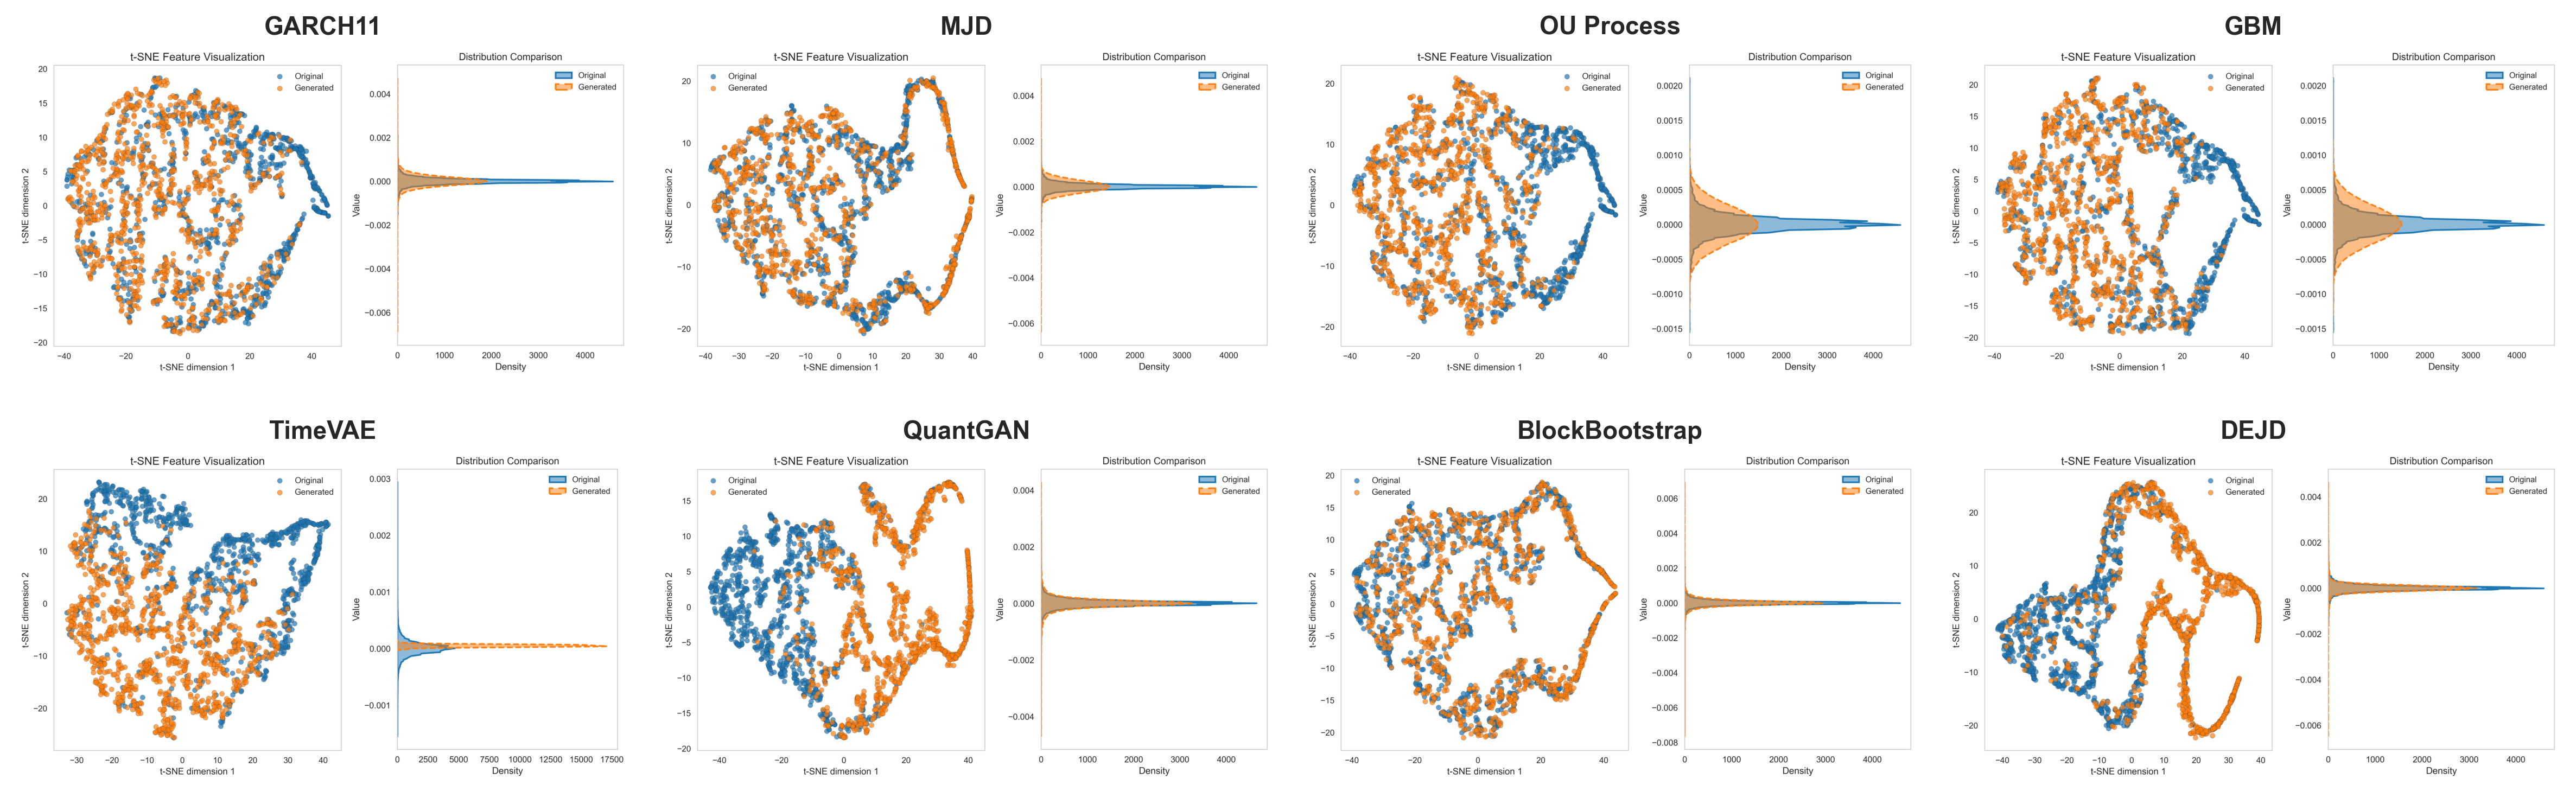
\includegraphics[width=\textwidth,height=8cm,keepaspectratio]
      {../../results/main_experiment/figure_2_tsne_distribution/figure_2_tsne_distribution.png}
      \caption{t-SNE visualization and distribution plots comparing real and synthetic financial time series data across models.
      (Specification: sequence length based on
      maximum significant PACF lag)}
      \Description{t-SNE embeddings and histograms showing the overlap and distributional properties of real versus synthetic data generated by different SDGFTS models.}
      \label{fig:tsne_distribution}
  \end{figure*}

  \subsection{Statistical Evaluation Results}\label{sec:stats_results}
    The following 2 sections are basesd on the results summarized in
    figure \ref{fig:heatmap_all_taxonomies}.
    \subsubsection{Stylized Facts and Fidelity}
    The block bootstrap \ref{alg:blockbootstrap2} consistently 
    achieves the strongest 
    performance across both distributional metrics and stylized facts. 
    This outcome is expected: by resampling contiguous blocks from the 
    training data, the block bootstrap directly inherits empirical 
    marginal distributions \ref{metric:mdd} and short- to 
    medium-range dependence 
    structures. As a result, it naturally preserves key stylized facts 
    (e.g., heavy tails \ref{metric:kd}, volatility clustering 
    \ref{metric:volclustering}) as long as they are present within 
    the chosen block length.

    Among parametric models, GARCH \ref{alg:garch} performs second 
    best overall. This is
    consistent with its widespread use in financial time series modeling:
    GARCH is explicitly designed to capture volatility clustering and
    volatility persistence. While standard GARCH models do not exhibit
    true long-memory behavior (in the strict statistical sense), they
    nonetheless approximate slowly decaying volatility autocorrelations
    well enough to score favorably on stylized-fact metrics relative to
    simpler parametric models such as OU process and GBM.

    The DEJD \ref{alg:dejd} model underperforms on kurtosis-
    based metrics \ref{metric:kd} despite its ability to generate fat tails.
    Although the jump component introduces excess kurtosis relative to pure
    diffusion processes, the model is not inherently calibrated to
    reproduce empirical tail thickness precisely. Its weaker performance
    likely reflects limitations in parameter estimation and
    mismatch between assumed jump dynamics and the empirical return
    distribution.

    Volatility models such as GBM \ref{alg:gbm} and the OU process \ref{alg:ou}
     perform poorly on
    stylized facts (§ \ref{sec:stylized-facts}). This result is unsurprising: 
    both models assume
    conditionally Gaussian increments with constant (GBM) or mean-reverting
    (OU) volatility, and therefore cannot reproduce volatility clustering
    or persistent heteroskedasticity observed in real financial time
    series.

    A notable result is that QuantGAN performs significantly worse on
    distributional metrics while capturing stylized facts relatively well.
    This suggests that the adversarial objective is effective at matching
    temporal dependence and higher-order dynamics, but less effective at
    aligning marginal distributions without explicit distributional
    constraints. TimeVAE performs poorly overall, which is consistent with
    posterior collapse when trained on log returns—limiting its ability to
    generate meaningful variability and capture higher-order financial
    structure.

    \subsubsection{Efficiency}

    Efficiency results largely follow model complexity. GBM, as the
    simplest model both conceptually and computationally, is the fastest
    to train and sample from. In contrast, QuantGAN is the slowest by
    design, reflecting the cost of adversarial training and high-capacity
    neural architectures.

    \subsubsection{Visualization}

    Figure \ref{fig:tsne_distribution} presents t-SNE embeddings and
    return distribution plots (see §\ref{sec:visualization_methods}) 
    for real versus synthetic data across
    models. The block bootstrap \ref{alg:blockbootstrap2}shows 
    near-perfect overlap in t-SNE space, reflecting its direct 
    resampling from real data. QuantGAN \ref{alg:quantgan} and
    DEJD \ref{alg:dejd} also shows better distribution alignment,
    but does not full capture the clusters in the t-SNE plots.

    While other parametric models do not capture these clusters fully,
    they generally corroborate the quantitative findings: GARCH
    \ref{alg:garch} shows better distributional alignment than GBM
    \ref{alg:gbm} and OU process \ref{alg:ou}, while TimeVAE
    \ref{alg:timevae} exhibits the worst overlap and distributional
    mismatch, as it appears to suffer from posterior collapse.

    \subsubsection{Diveristy metrics}\label{sec:diversity_introduce}

    Diversity alone is ambiguous: high variability does not guarantee
    realism and may violate structural dependencies. We therefore evaluate
    diversity jointly with fidelity to ensure variability remains
    plausible. We revisit this in research question \ref{rq:2} and in
    §\ref{sec:metric_tradeoffs}.
    
    \subsection{Utility Evaluation Results}\label{sec:hedger_results}
    \begin{figure*}[h]
      \centering
      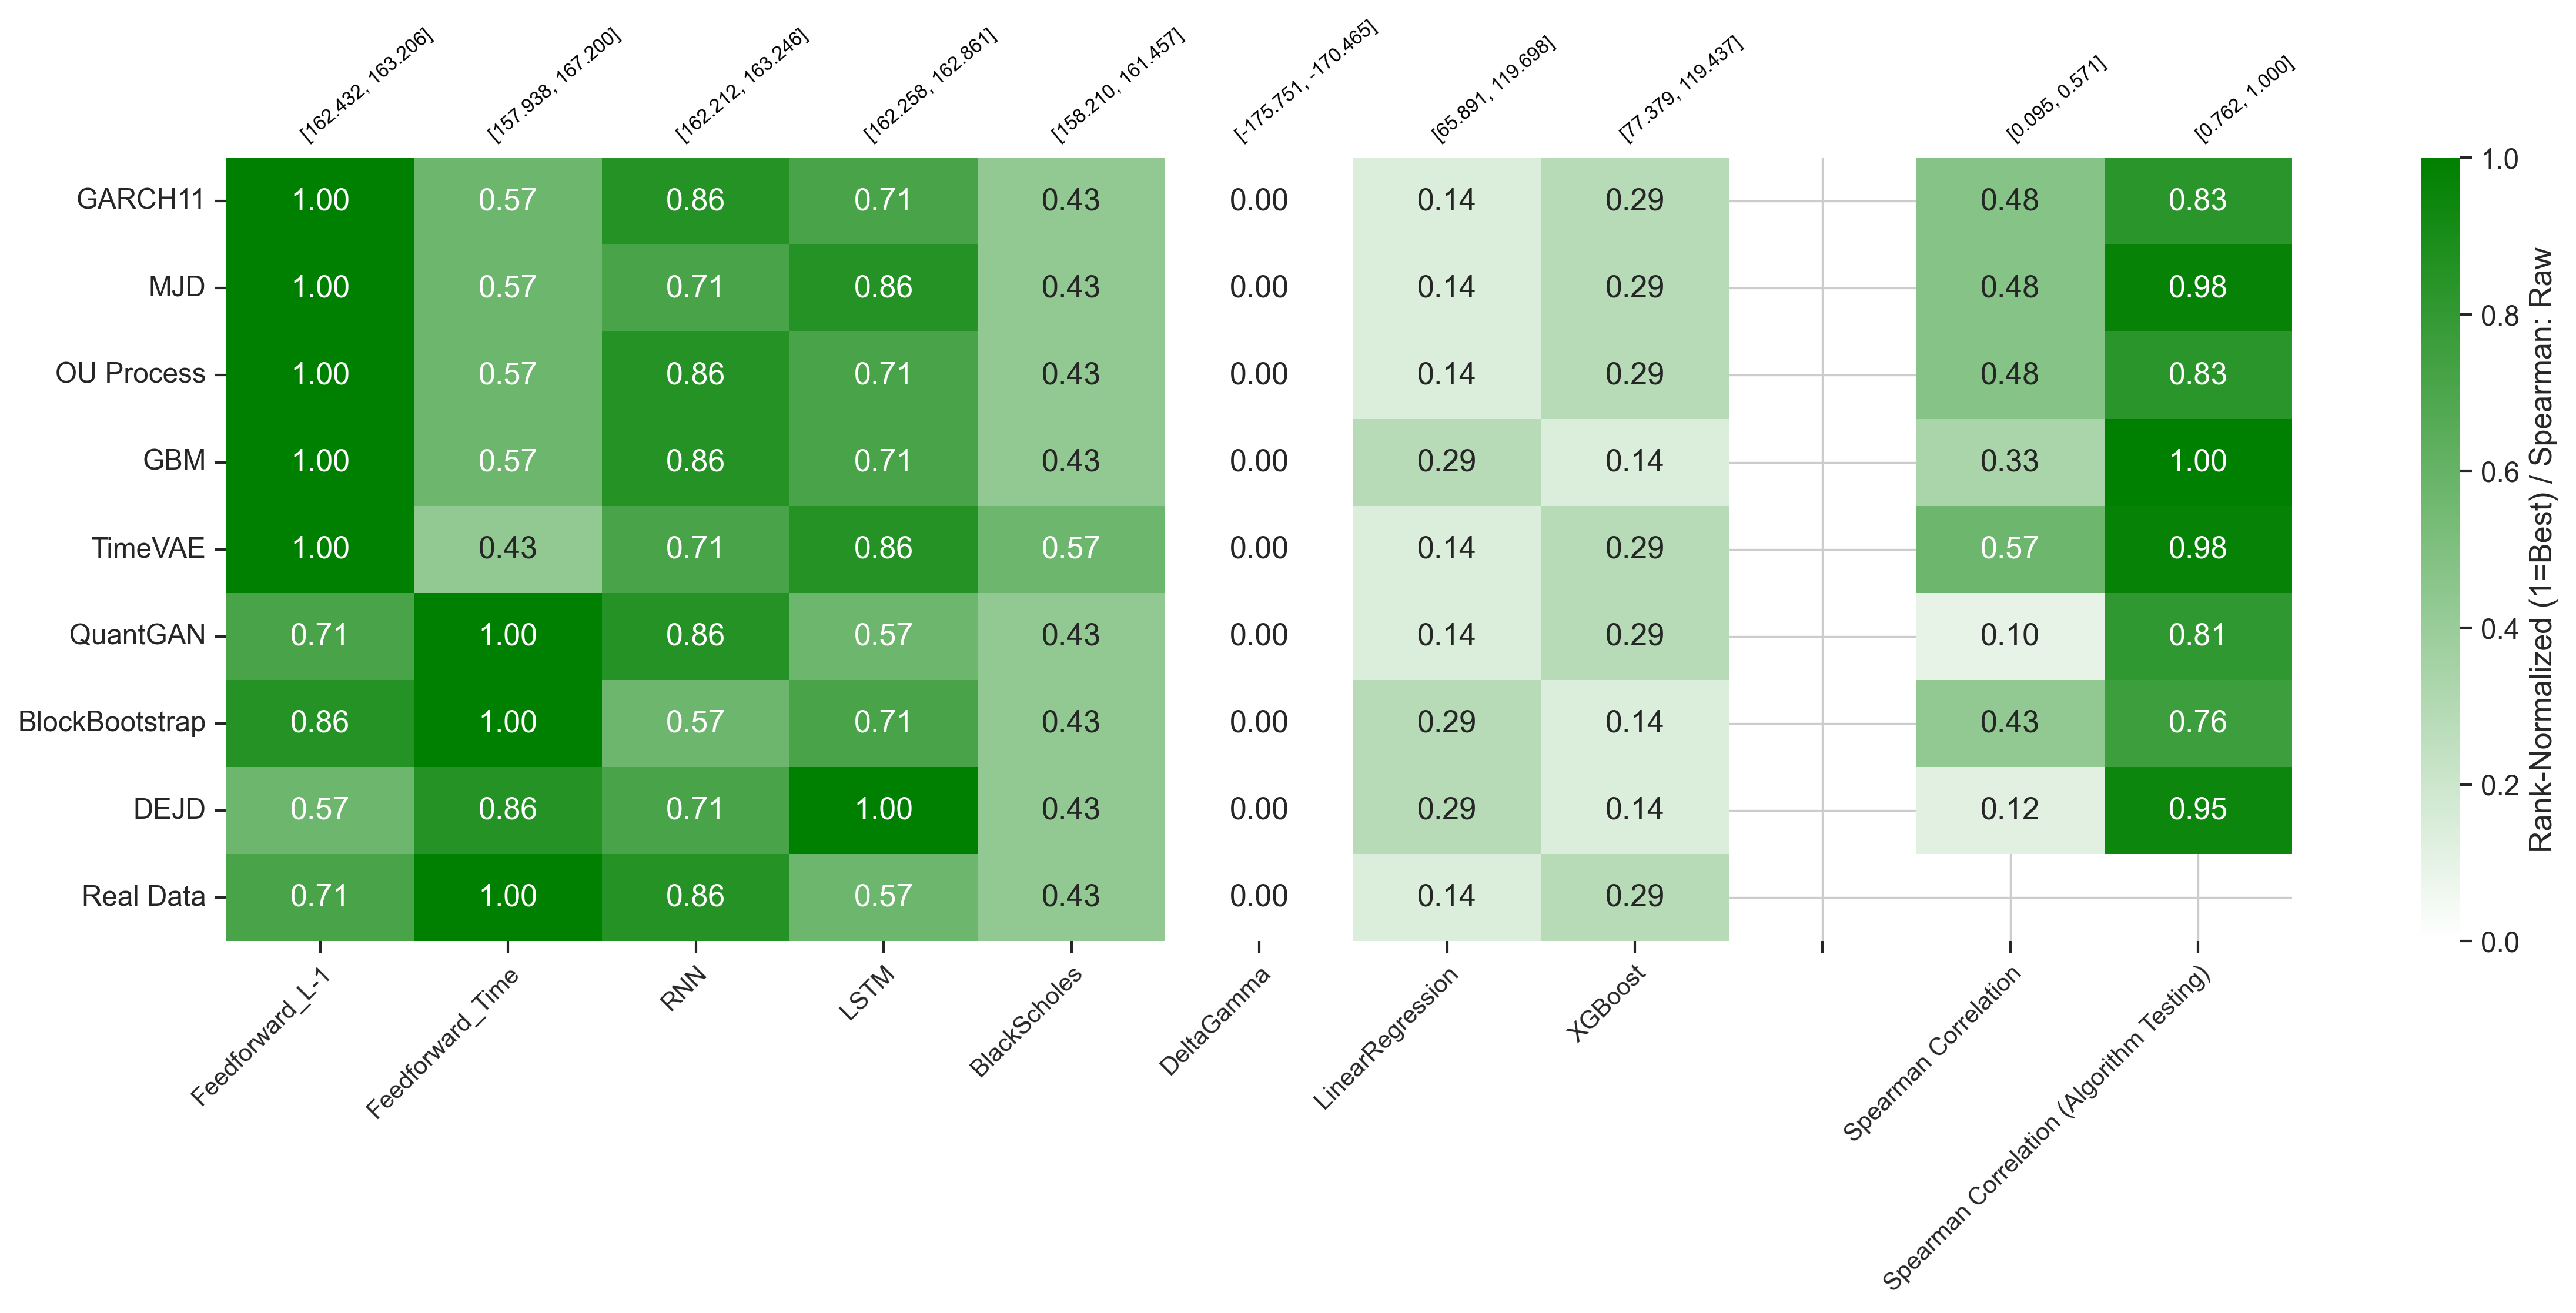
\includegraphics[width=\textwidth,height=8cm,keepaspectratio]
      {../../results/main_experiment/figure_1_per_metric_heatmaps/figure_1_utility_and_algorithm_ranknorm_heatmap.png}
      \caption{Normalized ranking heatmap for mean replication values
      of each hedger trained on SDGFTS/real data. Raw minimum and 
      maximum values are provided for each metric column.
     (Specification: Augmented datasets and sequence length based on
      maximum significant PACF lag).}
      \Description{Heatmap displaying normalized utility metric rankings 
      and algorithm comparison results across different SDGFTS models.}
      \label{fig:heatmap_utility_algorithm}
    \end{figure*}

    As see in Figure \ref{fig:heatmap_utility_algorithm},
    for the augmented testing \ref{sec:augmented-testing}, we can make the observation that for the
    hedging models, the neural network models generally perform better
    than the parametric models in estimating the deltas. This is expected
    as the neural network models are able to capture the higher-order
    dynamics of the index series, which the parametric models are not
    able to capture \cite{Fecamp20}.

    In the augmented-testing setting, with algorithms compared across
    datasets (see §\ref{sec:algorithm-comparison}), we observe that
    the rank-normalized values of the
    heatmaps obtained using QuantGAN \ref{alg:quantgan}
    and BlockBootstrap \ref{alg:blockbootstrap2}
     remain highly consistent with those derived from real-only
    data. In particular, rank-normalized hedging performance under
    QuantGAN augmentation closely matches the baseline ordering, while
    BlockBootstrap augmentation yields nearly identical results. This
    behavior is expected for BlockBootstrap, which preserves empirical
    dependence structures by construction, and suggests that
    QuantGAN-generated samples do not distort the hedger-relevant
    dynamics when mixed with real data. Thus, both augmentation
    strategies maintain the relative sensitivities and preferences of
    hedger models observed under real-data training, indicating that
    these synthetic generators can be used for augmentation without
    materially altering hedging-based performance assessments.

    For Spearman correlation (see Equation \ref{eq:Spearman}),
    recommended by Stenger et al., it's important to note that this metric
    considers only the ranking of model performances, completely ignoring
    the actual delta values between them \cite{Stenger24}. This can be 
    problematic: for
    example, TimeVAE \ref{alg:timevae} \textemdash despite suffering 
    from mode collapse and generating
    less realistic outputs \textemdash may still achieve a high Spearman correlation
    if it preserves the order of model performances, even though the
    deltas may be substantially off or meaningless. Conversely, QuantGAN,
    which better captures the structure of financial data, might produce
    more realistic values but achieve a worse Spearman score if the
    ranking changes slightly. Thus, relying solely on Spearman
    correlation can be misleading, as it overlooks the magnitude and
    quality of differences between models and may obscure meaningful
    distinctions in model performance.
  
  \subsection{\ref{rq:1} Metric Response on Sequence Length Training}
    We investigate how training sequence length affects evaluation
    metrics as posed in research question \ref{rq:1}.
    As previous sections describe how sequence length is determined
    based on model-specific PACF analysis (§\ref{sec:model-specific})
    how they affect the Stonk Bench architecture.

    Recall that the sequence lengths considered are 60, 120, 180, 240,
    and 300 minutes respectively.

  We analyze each metric as the training sequence length varies from
  60 to 300 minutes.

\subsubsection{Fidelity}
  Rank-normalized MDD values are essentially invariant to sequence
  length, which is expected for a marginal distribution metric unless
  models generate time-varying distributions (not observed here).
  Skewness differences show minimal variation for GARCH(1,1), GBM, OU,
  and MJD, suggesting limited sensitivity to sequence length. Modest
  rank improvements for BlockBootstrap and DEJD likely reflect better
  capture of asymmetric tail events. Kurtosis differences for GARCH,
  MJD, OU, and GBM change marginally with sequence length, consistent
  with limited extreme-tail generation; BlockBootstrap improves with
  longer sequences by resampling rare extremes. See the fidelity
  ablation heatmap in Figure~\ref{fig:ablation_fidelity}.

\subsubsection{Diversity}
  Diversity rankings remain stable across sequence lengths, consistent
  with largely unchanged marginal distributions. However, the minimum
  and maximum diversity values increase with sequence length, as longer
  windows permit greater variability across time steps. See the
  diversity ablation heatmap in Figure~\ref{fig:ablation_diversity}.

\subsubsection{Efficiency}
  Maximum generation time increases monotonically with sequence length,
  while model rankings remain unchanged, reflecting computational
  complexity rather than algorithmic reordering. See the efficiency
  ablation heatmap in Figure~\ref{fig:ablation_efficiency}.

\subsubsection{Stylized facts}
  The maximum values for lag-1 autocorrelation of absolute returns and
  volatility clustering increase with sequence length, whereas long
  memory measures tend to decrease. Rankings for QuantGAN,
  BlockBootstrap, and DEJD are largely preserved across lengths. See
  the stylized-facts ablation heatmap in
  Figure~\ref{fig:ablation_stylized_facts}.

\subsubsection{Spearman correlation}
  Spearman's rank correlation summarizes ordering only and can be
  misleading when magnitude differences matter; reliance on it alone is
  therefore discouraged. See the utility correlation comparison in
  Figure~\ref{fig:ablation_utility_spearman}.


  \subsection{\ref{rq:2} Metric Tradeoffs and Interactions}
  \label{sec:metric_tradeoffs}
    We dedicate this subsection to answer the research question
    \ref{rq:2} regarding trade-offs and interactions between different
    evaluation metrics.

    \subsubsection{Diversity versus Fidelity}
      As introduced in §\ref{sec:diversity_introduce}, diversity
      metrics must be interpreted in conjunction with fidelity and
      stylized-fact metrics. How should we interpret these relationships? 
      Recall that "difference" here means the discrepancy between real 
      and synthetic data—the lower the value, the better the model is 
      matching the real data.

      The MDD \ref{metric:mdd} and SDD \ref{metric:sdd} 
      both show a notably strong positive correlation with ICD 
      Euclidean diversity \ref{metric:ed}. For example, MDD has a 
      Pearson correlation coefficient of \( r = 0.68 \) (p = 0.09), 
      and STD difference has an even higher \( r = 0.97 \) 
      (p = 1.90e-4) (see Figure \ref{fig:eclidian_fidelity_diversity}). 
      This indicates that as the marginal or standard deviation 
      difference between real and synthetic data increases (i.e., as 
      fidelity to the real data worsens), the diversity, as measured 
      by ICD Euclidean, also tends to increase.

      The findings indicate that increased diversity, as measured by ICD 
      Euclidean, often correlates with reduced fidelity in basic 
      distributional statistics. This suggests that models generating 
      more diverse samples may deviate significantly from the real data 
      distribution, highlighting the necessity of balancing diversity 
      with fidelity. While some diversity is beneficial for generative 
      models, excessive diversity can lead to less realistic outputs. 
      Therefore, it is crucial to evaluate both fidelity and diversity 
      metrics together when assessing generative time series models.

    \subsubsection{Diversity versus Stylized Facts}
      Figure \ref{fig:eclidian_stylized_facts_diversity} presents
      scatter plots illustrating the relationship between ICD Euclidean
      diversity \ref{metric:ed} and key stylized-fact metrics:
      ACD \ref{metric:acd}, volatility clustering \ref{metric:volclustering},
      and LMSD \ref{metric:slow_decay}.

      Volatility clustering shows a weak positive correlation with
      diversity (p \( \approx \) 0.1). This suggests that more diverse models
      tend to preserve stronger volatility clustering, indicating
      that allowing a broader range of sample paths may help retain
      persistent volatility dynamics, though the evidence is
      marginal.

      Long memory in volatility is also positively and mildly
      correlated with diversity. This implies that models producing
      more varied samples are more likely to exhibit persistent,
      slowly decaying volatility correlations, consistent with
      richer temporal dynamics emerging from increased generative
      flexibility.

    \begin{figure}[h]
      \centering
      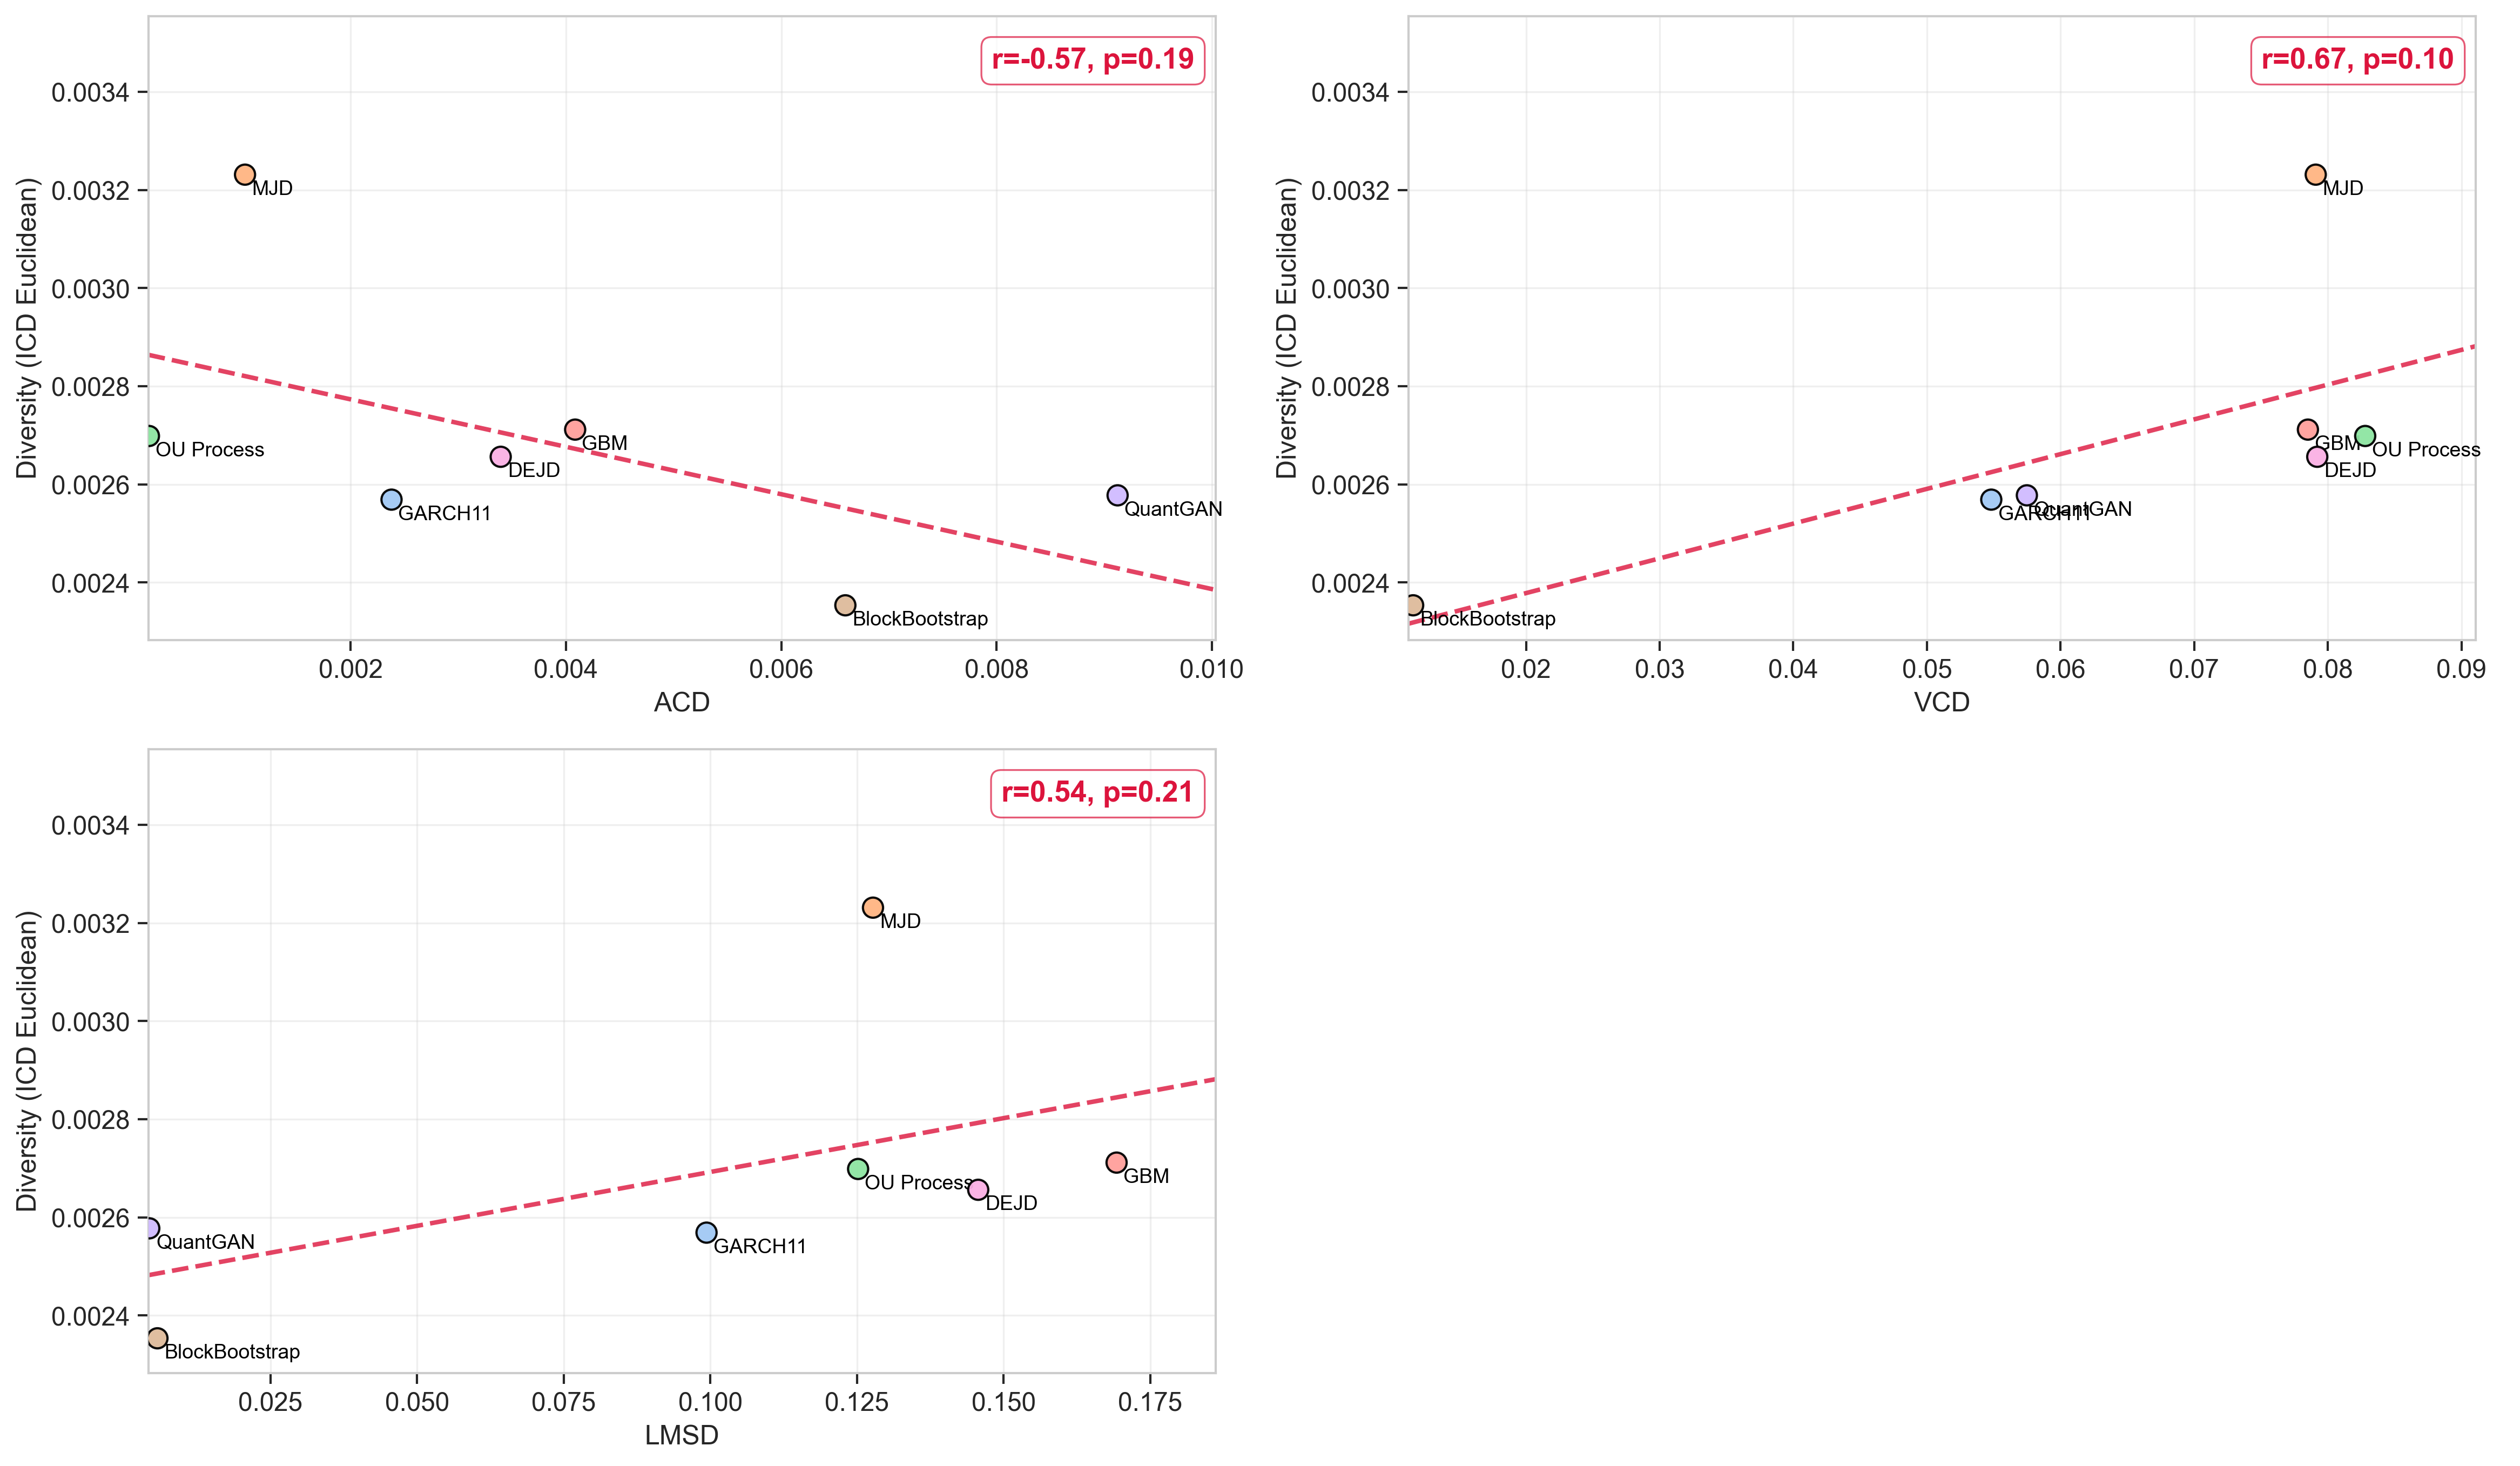
\includegraphics[width=0.45\textwidth,height=6cm,keepaspectratio]
      {../../results/appendix/figure_6_stylized_facts_vs_diversity/figure_6_icd_euclidean_2x2_grid.png}
      \caption{Scatter plots showing the relationship between 
      ICD Euclidean diversity and stylized facts metrics (ACD, 
      volatility clustering, and LMSD). Each point represents a model, 
      with trend lines indicating correlation direction and strength.}
      \Description{Scatter plots illustrating the correlation between 
      ICD Euclidean diversity and stylized facts metrics (ACD, 
      volatility clustering, and LMSD)
      across different models.}
      \label{fig:eclidian_stylized_facts_diversity}
    \end{figure}

    \subsubsection{Efficiency versus other metrics}
      Efficiency, measured by generation time, shows no significant
      correlation with fidelity, diversity, or stylized-fact metrics.
      This indicates that faster models do not necessarily compromise
      on quality or realism, nor do slower models guarantee better
      performance. Thus, efficiency appears to be largely independent
      of other evaluation dimensions in this benchmark.


% \section{Conclusion and Future Work}
  In our research, we recognize the existing limitations in the
    evaluation of synthetic time series, particularly the absence of a
    universally accepted framework. To address this, we adopt the
    evaluation taxonomy proposed by Stenger et al. and expand upon it to
    create a comprehensive benchmark specifically tailored for Synthetic
    Data Generation for Financial Time Series (SDGFTS).
    Our contributions include the development of a consolidated evaluation
    framework that systematically reviews and integrates various
    assessment methods from leading studies in the field. This approach
    not only enhances the rigor of evaluations but also facilitates the
    comparison of different SDGFTS models, ultimately providing a more
    standardized and reliable means of assessing synthetic data quality.

  We believe that Stonk Bench will serve as a valuable resource for
    researchers and practitioners in the field of synthetic financial
    time series generation.
    We hope that our benchmark will facilitate more rigorous and
    standardized evaluations of SDGFTS models, ultimately advancing
    the state of the art in this important area of research.
    For the broader field of synthetic data generation, our work
    highlights the importance of a comprehensive and unifying
    evaluation frameworks that consider both statistical properties
    and practical utility that is proposed by Stenger \textit{et al.}.
  \subsection{Summary of Findings}
  We presented Stonk-Bench, a comprehensive benchmark for evaluating 
  Synthetic Data Generation for Financial Time Series (SDGFTS). This 
  benchmark integrates statistical fidelity, diversity, stylized facts 
  verification, and utility evaluation through (deep) hedging. We evaluated 
  a suite of 5 traditional, 3 deep learning-based, and 1 other SDGFTS 
  models on the S\&P 500 minute-level dataset.
  \subsection{Stonk Bench Shortcomings}\label{subsub:shortcomings}
      While Stonk Bench represents a significant step forward in the
      evaluation of SDGFTS models, we acknowledge several limitations
      in our current work:
    \begin{enumerate}[label=\textbf{[S\arabic*]}]
      \item \textbf{Incompatibility with other models:}
        Stonk Bench has so far been evaluated mainly on classical
        stochastic models (e.g., GBM, OU, GARCH) and a subset of
        deep-learning approaches (GANs, VAEs).
        Other model families — such as
        reinforcement-learning-based generators, normalizing flows,
        autoregressive networks, and hybrid methods — have not yet
        been benchmarked.
      \item \textbf{No hyperparameter tuning:} For consistency and
        comparability across models, StonkBench evaluations were
        performed using default model configurations, without
        performing hyperparameter optimization. This ensures a fair
        baseline but may not reflect the absolute best performance
        achievable by each model.
      \item \textbf{Metric and procedure generalizability:}
        As a consequence, some metrics or evaluation procedures may
        not directly translate to these untested families, which
        limits the framework's generalizability across all synthetic
        financial time-series generation methods.
      \item \textbf{Data Leakage from Public Datasets:} Current models
        can potentially overfit to publicly available datasets
        \textemdash the same datasets that Stonk Bench is using
        \textemdash leading to inflated performance metrics that do
        not generalize well to unseen data. One possible solution is
        to either curate proprietary datasets or implement a grace
        period so the model can be tested on new data that was not
        publicly available during its development.
      \item \textbf{Computational Resource Requirements:} The
        comprehensive nature of Stonk Bench \textemdash particularly
        accommodating any submitted (deep) hedging model and the deep
        hedging utility evaluation \textemdash demands significant
        computational resources. This may limit accessibility for
        researchers with constrained resources.
    \end{enumerate}
  \subsection{Future Research Directions}
    \subsubsection{Remaining progress} In regard to the next portion
    of our project, we aim to expand Stonk Bench in several key areas.
    \begin{enumerate}[label=\textbf{[F\arabic*]}]
      \item \textbf{Multivariate time series predictions.}
        Extend Stonk Bench to evaluate models on multivariate time
        series data, enabling a more comprehensive assessment of their
        performance in realistic scenarios. We wish test SDGFTS models
        on datasets with multiple correlated assets and datasets with
        Bid-Ask spreads and trading volume to evaluate their ability to
        capture inter-asset dependencies and market microstructure
        effects \cite{Takahashi24}.
        \item \textbf{Data granularity evaluation.}
        We wish to test SDGFTS models across multiple data granularities
        (minute-level, daily, and weekly) to evaluate model performance
        on different temporal scales and their ability to capture both
        short-term and long-term dependencies. The most relevant granularities
        that are commonly used in financial analysis and trading strategies
        are 5-minute, 30-minute, and daily data \cite{Wang20, Cont01}.
    \end{enumerate}

    \subsubsection{Beyond the project} We envision Stonk Bench
    evolving into a community-driven benchmark for SDGFTS evaluation.
    As we acknowledge the shortcomings outlined in
    §\ref{subsub:shortcomings}, we propose the following future
    directions:
    \begin{enumerate}[label=\textbf{[F\arabic*]}, resume]
      \item \textbf{Continuous model inclusion.}
      Maintain Stonk Bench as a living benchmark by incorporating
      newly developed SDGFTS techniques (normalizing flows,
      autoregressive generators, advanced diffusion models,
      reinforcement-learning-based generators, and hybrids)
      \cite{Potluru24}.
      \item \textbf{Rigorous metric selection and ablations.}
      As mentioned in Stenger et al., we wish to rigorously conduct
      ablation studies to identify the most informative and robust
      metrics for different model families and stylized facts;
      produce guidance for a compact, interpretable metric set
      \cite{Stenger24}.
      \item \textbf{Categories of datasets} We wish to format Stonk
      Bench to cover a variaty datasets categorized by asset class (
      equities, forex, commodities, cryptocurrencies), 
      granularity (minute, five-minute, daily), and datatypes (OHCL,
      BAV).
      \item \textbf{Public benchmark platform.}
      Launch a website with documentation, code, datasets, and a
      leaderboard for submitted SDGFTS models; provide CI-enabled
      evaluation pipelines for reproducible comparisons.
      \item \textbf{Community engagement.}
      Foster collaboration via contribution guidelines, open issues,
      and reproducible example workflows so researchers can extend
      and validate the benchmark.
    \end{enumerate}

\begin{acks}
  To professor Irene Huang, University of Toronto, for her
  supervision and guidance throughout the project.
\end{acks}





\bibliographystyle{ACM-Reference-Format}
\bibliography{stonk-bench}

\appendix

% \section{Utility Evaluation Logistics}
  Detailed procedures for (deep) hedging evaluation, including
  dataset splits, model architectures, training hyperparameters,
  and evaluation metrics.

  \subsection{Hedging Tasks Specifications}
    We consider the hedging of a European call option on a single
    underlying asset \( S_t \) with strike price \( K \) and
    maturity \( T \). The option payoff at maturity is given by
    \( g(S_T) = \max(S_T - K, 0) \).

    For each sequence length tested in §\ref{sec:sequence_length},
    we have set the corresponding option maturity \( T \) to match
    the length of the generated sequences. For example, if the
    sequence length is 60 minutes, then the option maturity \( T \)
    is set to 60 minutes.

  \subsection{Algorithm Comparison Models}\label{appendix:deep-hedger-algorithms}
    In §\ref{sec:algorithm-comparison}, we described the procedure
    for comparing multiple (deep) hedger algorithms to evaluate the
    relative performance preservation on synthetic data versus real
    data.
  
      We have considered the following deep hedger algorithms:
      \begin{enumerate}[label=\textbf{[H\arabic*]}]
        \item \label{hedger:feedforwardlag} \textbf{Feedforward Layers
        Neural 
        Network (FLNN).} A standard multi-layer perceptron with 
        fully connected layers, ReLU activations, and dropout for 
        regularization.

        \item \label{hedger:feedforward} \textbf{Feedforward Time
        Neural Network (FTNN).} A feed-forward neural network designed 
          to process time series data by accepting lagged observations 
          as input features. This architecture uses fully connected 
          layers with ReLU activations and dropout for regularization, 
          enabling it to learn non-linear relationships between past 
          and future values without explicit recurrence.
        
        \item \label{hedger:lstm} \textbf{Long Short-Term Memory 
        (LSTM).} A recurrent neural network architecture designed 
        to capture temporal dependencies in sequential data, 
        particularly effective for time series tasks.
        
        \item \label{hedger:rnn} \textbf{Recurrent Neural Network (RNN).}
        An attention-based architecture that models long-range 
        dependencies in sequences without relying on recurrence, 
        utilizing self-attention mechanisms to enhance performance 
        on sequential data.
      
      \end{enumerate}
    
    We also considered the following (non-deep) hedging models:
    \begin{enumerate}[label=\textbf{[H\arabic*]}, resume]
      \item \label{hedger:black-scholes} \textbf{Black-Scholes 
      Delta Hedging (BSD).} A classical hedging strategy based on the 
      Black-Scholes option pricing model, which computes the 
      delta of the option to determine the optimal hedge ratio.

      \item \label{hedger:binomial} \textbf{Binomial Delta-Gamma Hedging (BDG).}
      A discrete-time hedging strategy that uses a binomial tree
      model to compute both delta and gamma of the option, allowing
      for more accurate hedging in the presence of non-linear price
      movements.

      \item \label{hedger:lreg} \textbf{Linear Regression Hedging (LR).} 
      A hedging strategy that uses linear regression to estimate 
      the hedge ratios based on historical data.

      \item \label{hedger:xgboost} \textbf{XGBoost Hedging (XGB).}
      A machine learning-based hedging strategy that employs
      gradient boosting decision trees to learn optimal hedge ratios
      from historical data.  
    \end{enumerate}

\begin{figure*}[h]
  \centering
  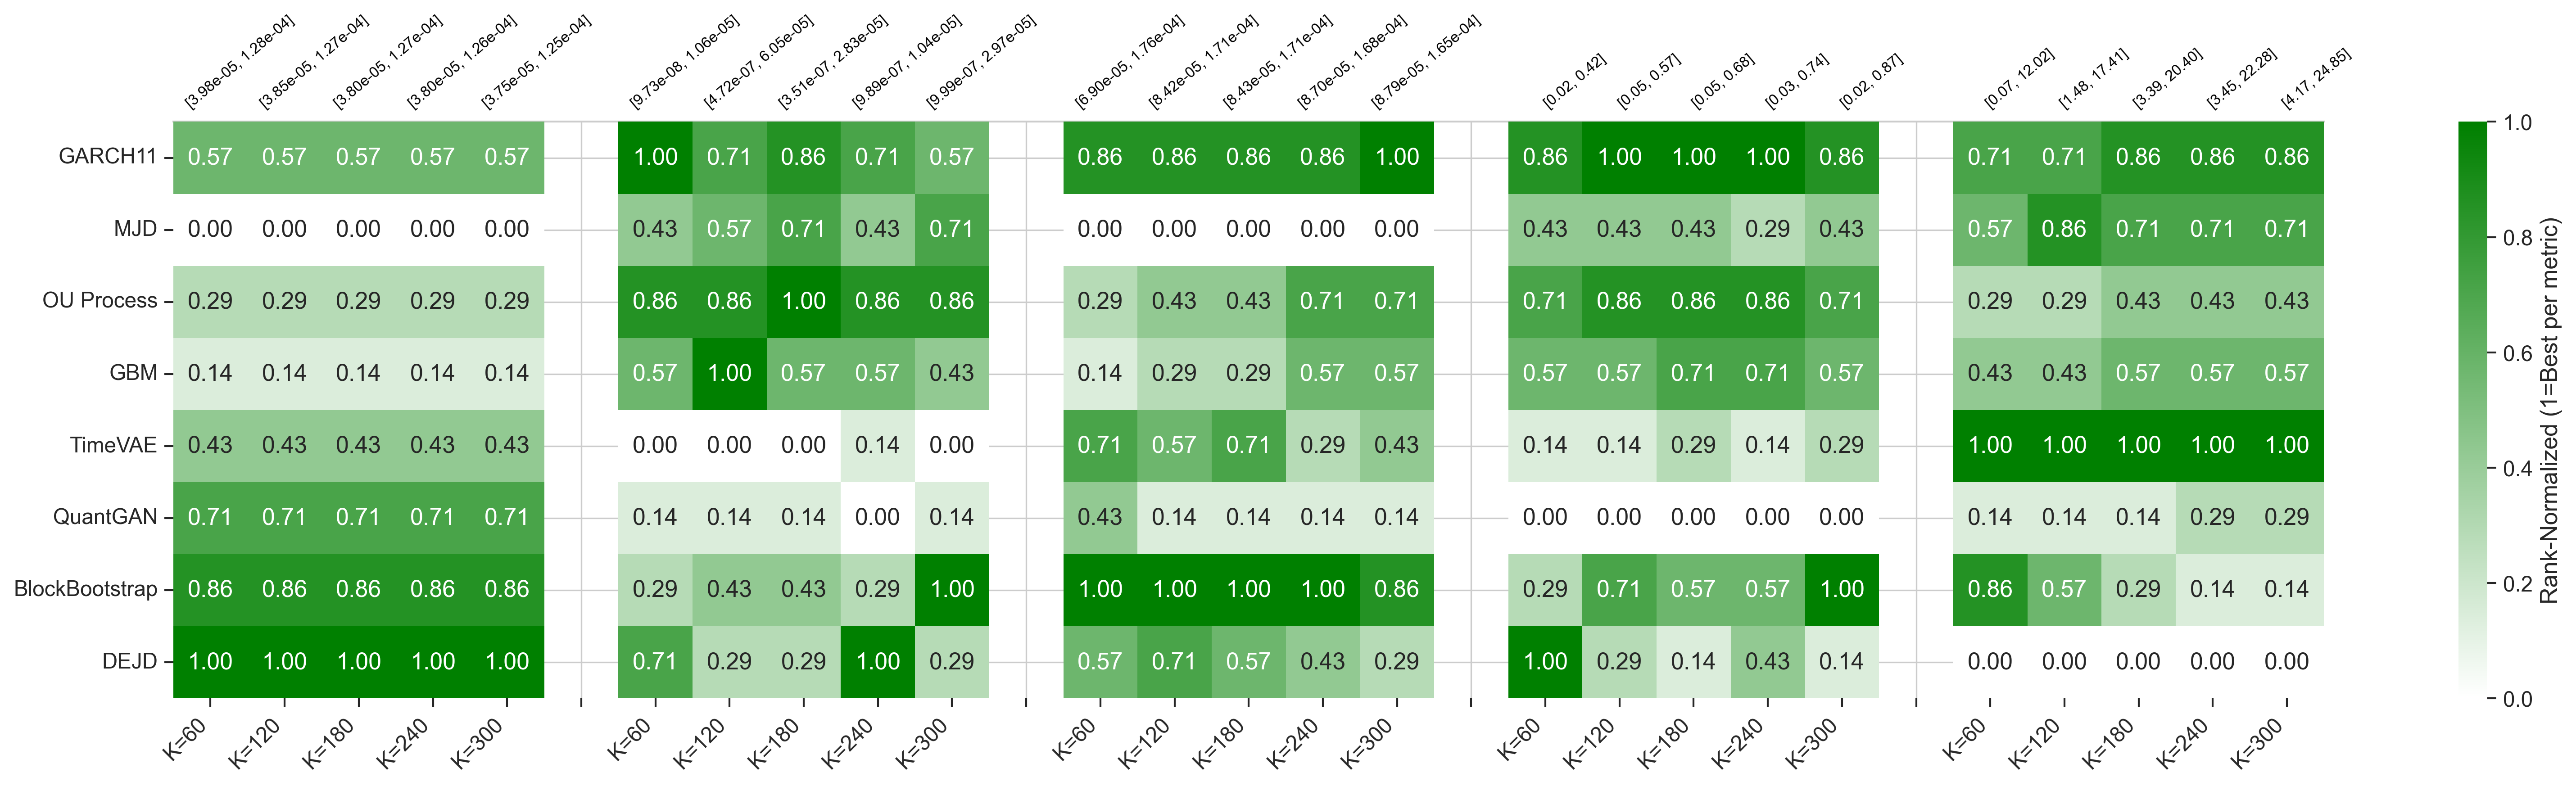
\includegraphics[width=0.9\textwidth,keepaspectratio]
  {../../results/ablation_studies/figure_3_metric_heatmaps_per_metric/figure_3_fidelity_per_metric_ranknorm.png}
  \caption{Ablation study: fidelity per-metric rank-normalized heatmap across sequence lengths.}
  \Description{Heatmap showing fidelity metrics across sequence length ablations.}
  \label{fig:ablation_fidelity}
\end{figure*}

\begin{figure*}[h]
  \centering
  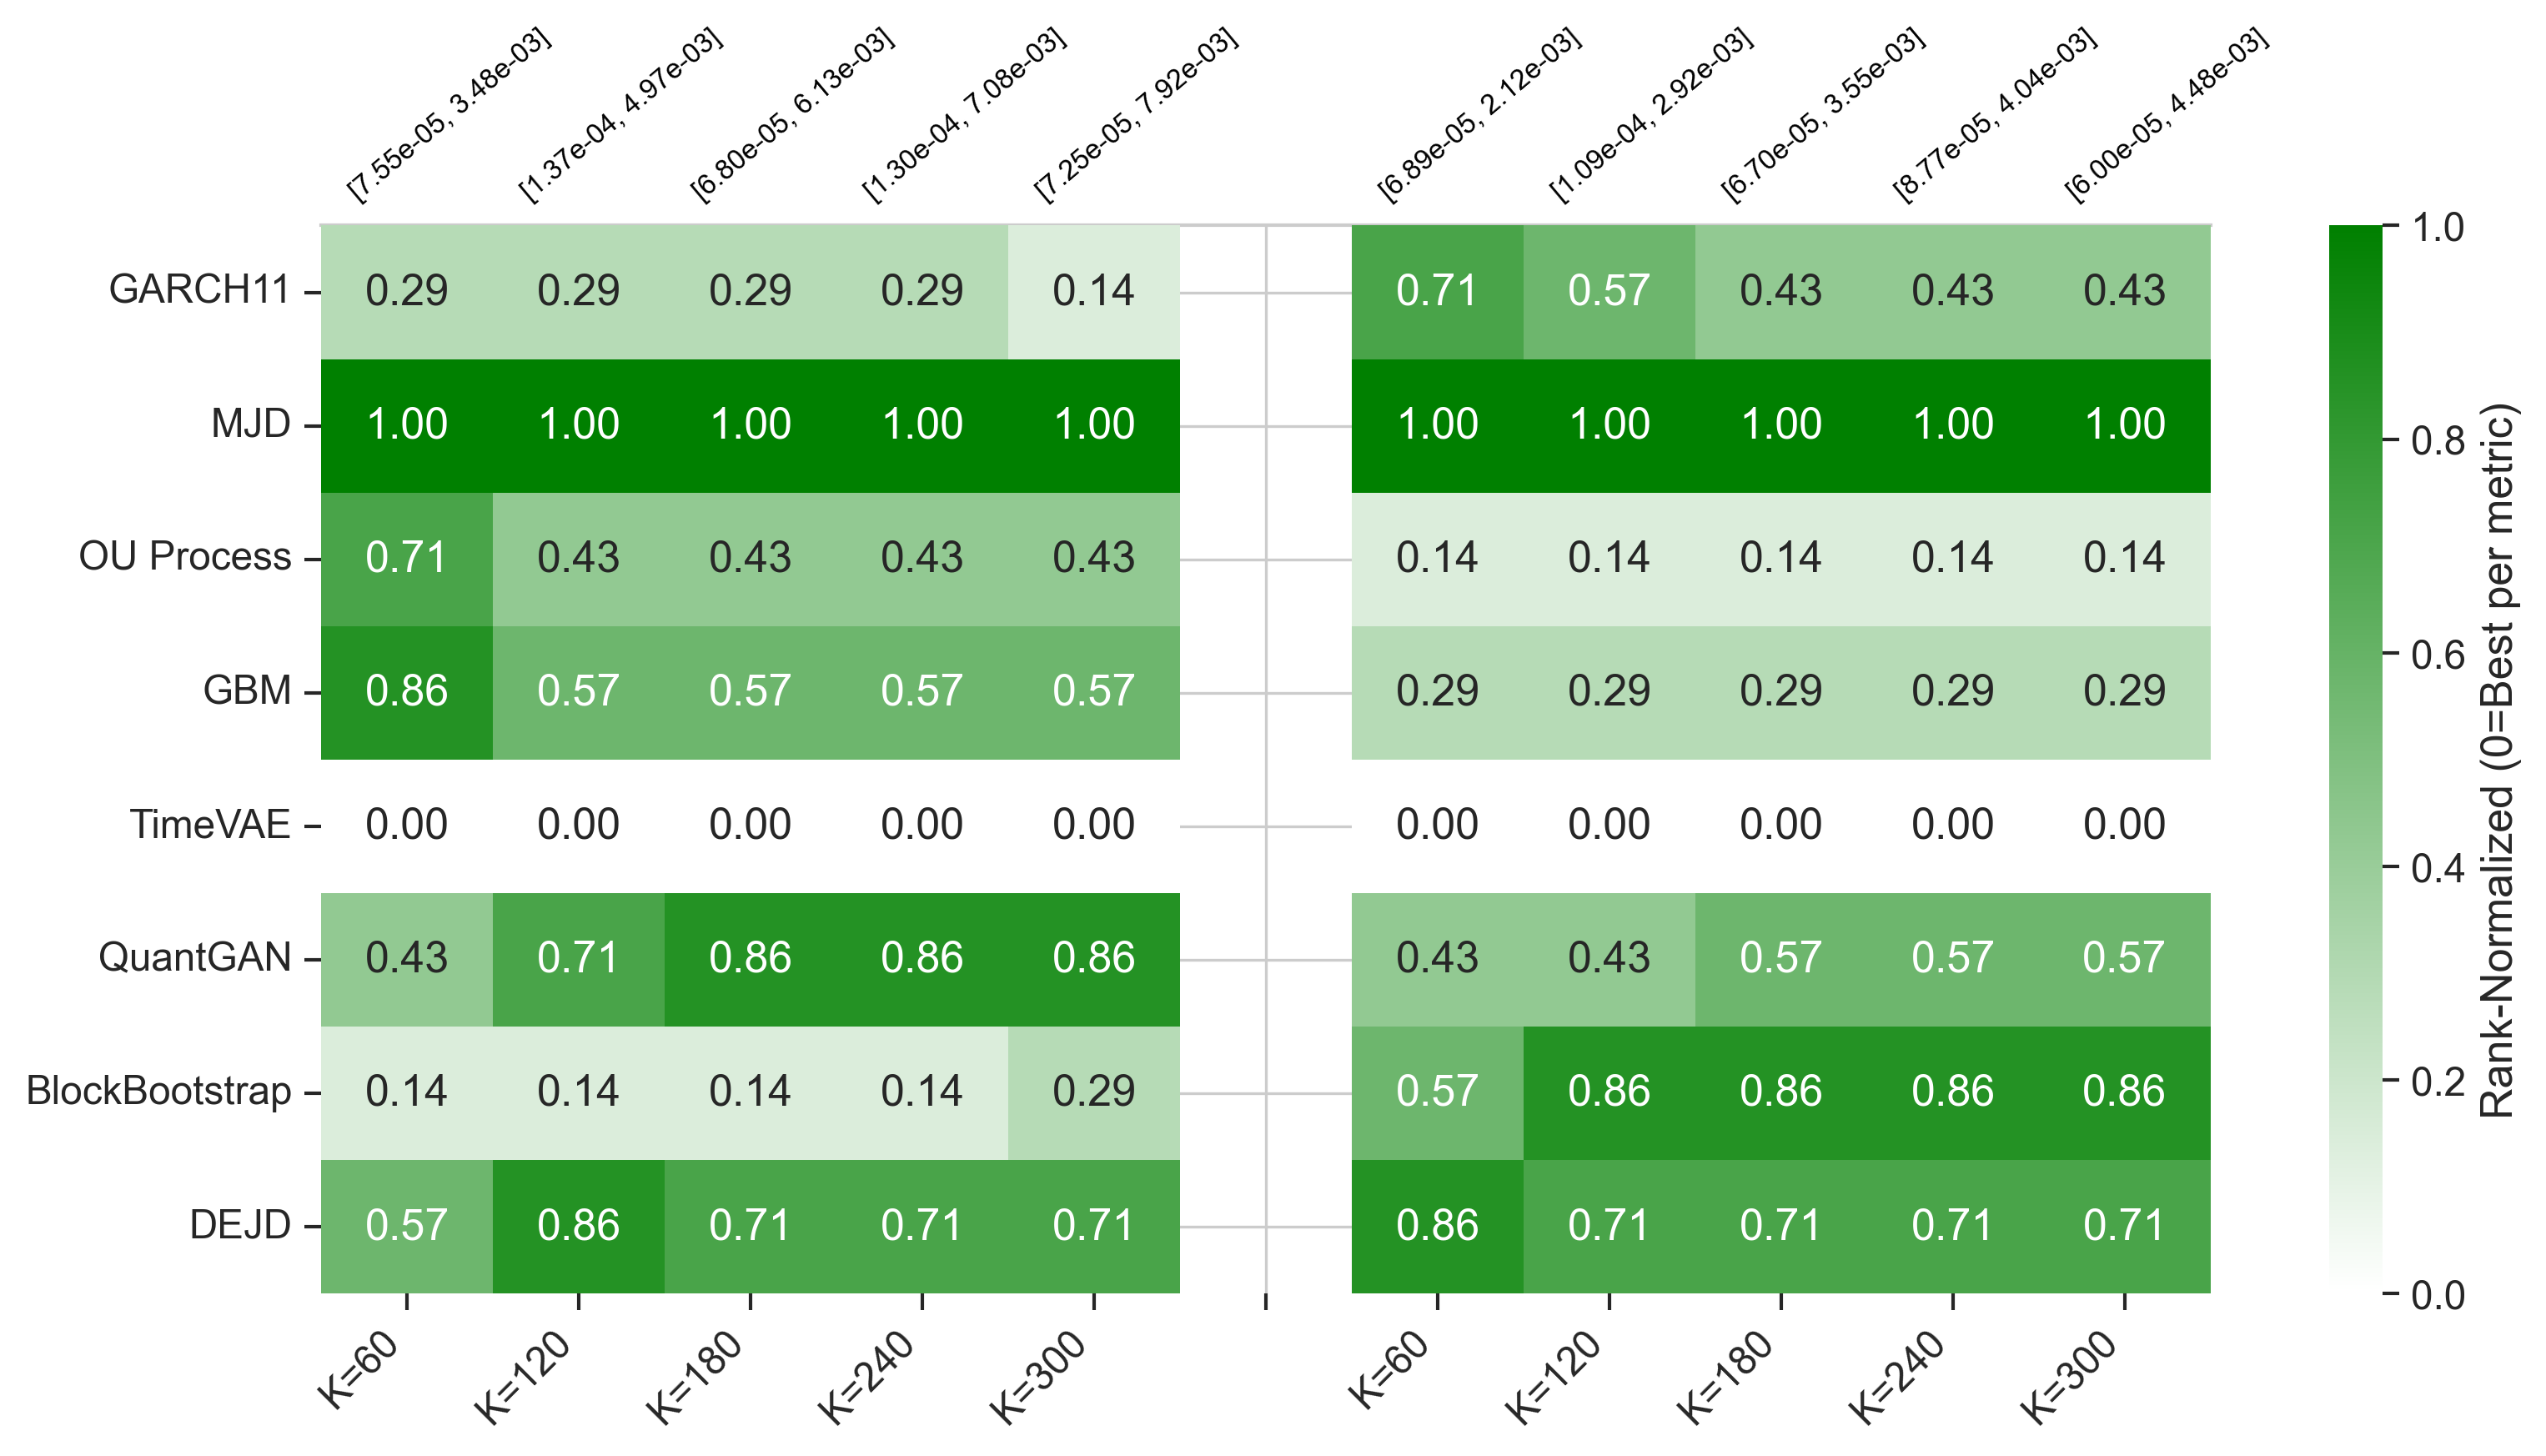
\includegraphics[width=0.9\textwidth,keepaspectratio]
  {../../results/ablation_studies/figure_3_metric_heatmaps_per_metric/figure_3_diversity_per_metric_ranknorm.png}
  \caption{Ablation study: diversity per-metric rank-normalized heatmap across sequence lengths.}
  \Description{Heatmap showing diversity metrics across sequence length ablations.}
  \label{fig:ablation_diversity}
\end{figure*}

\begin{figure*}[h]
  \centering
  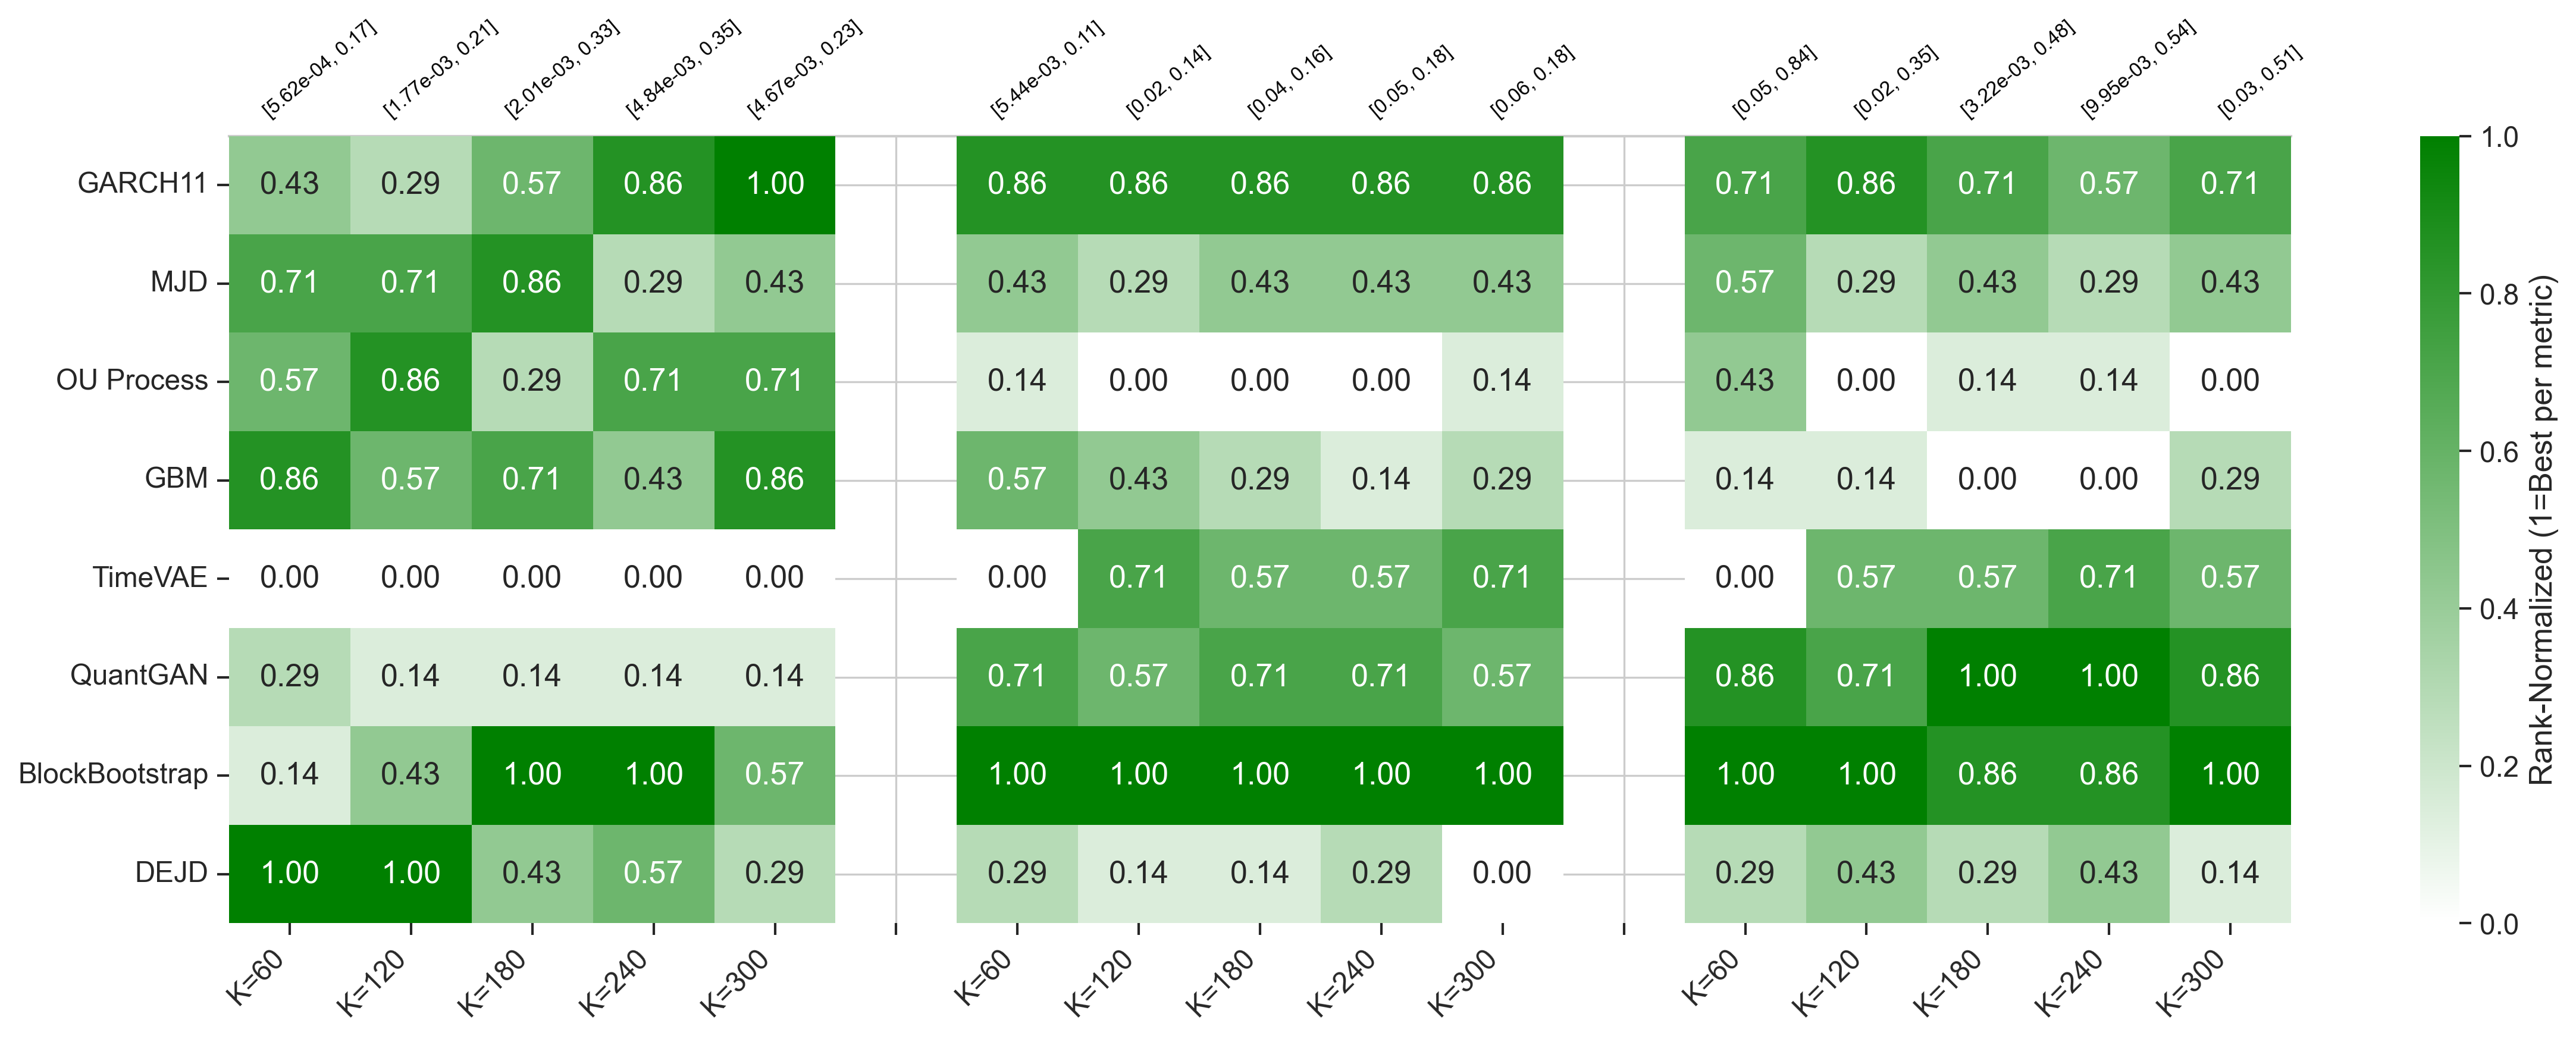
\includegraphics[width=0.9\textwidth,keepaspectratio]
  {../../results/ablation_studies/figure_3_metric_heatmaps_per_metric/figure_3_stylized-facts_per_metric_ranknorm.png}
  \caption{Ablation study: stylized-facts per-metric rank-normalized heatmap across sequence lengths.}
  \Description{Heatmap showing stylized-facts metrics across sequence length ablations.}
  \label{fig:ablation_stylized_facts}
\end{figure*}

\begin{figure*}[h]
  \centering
  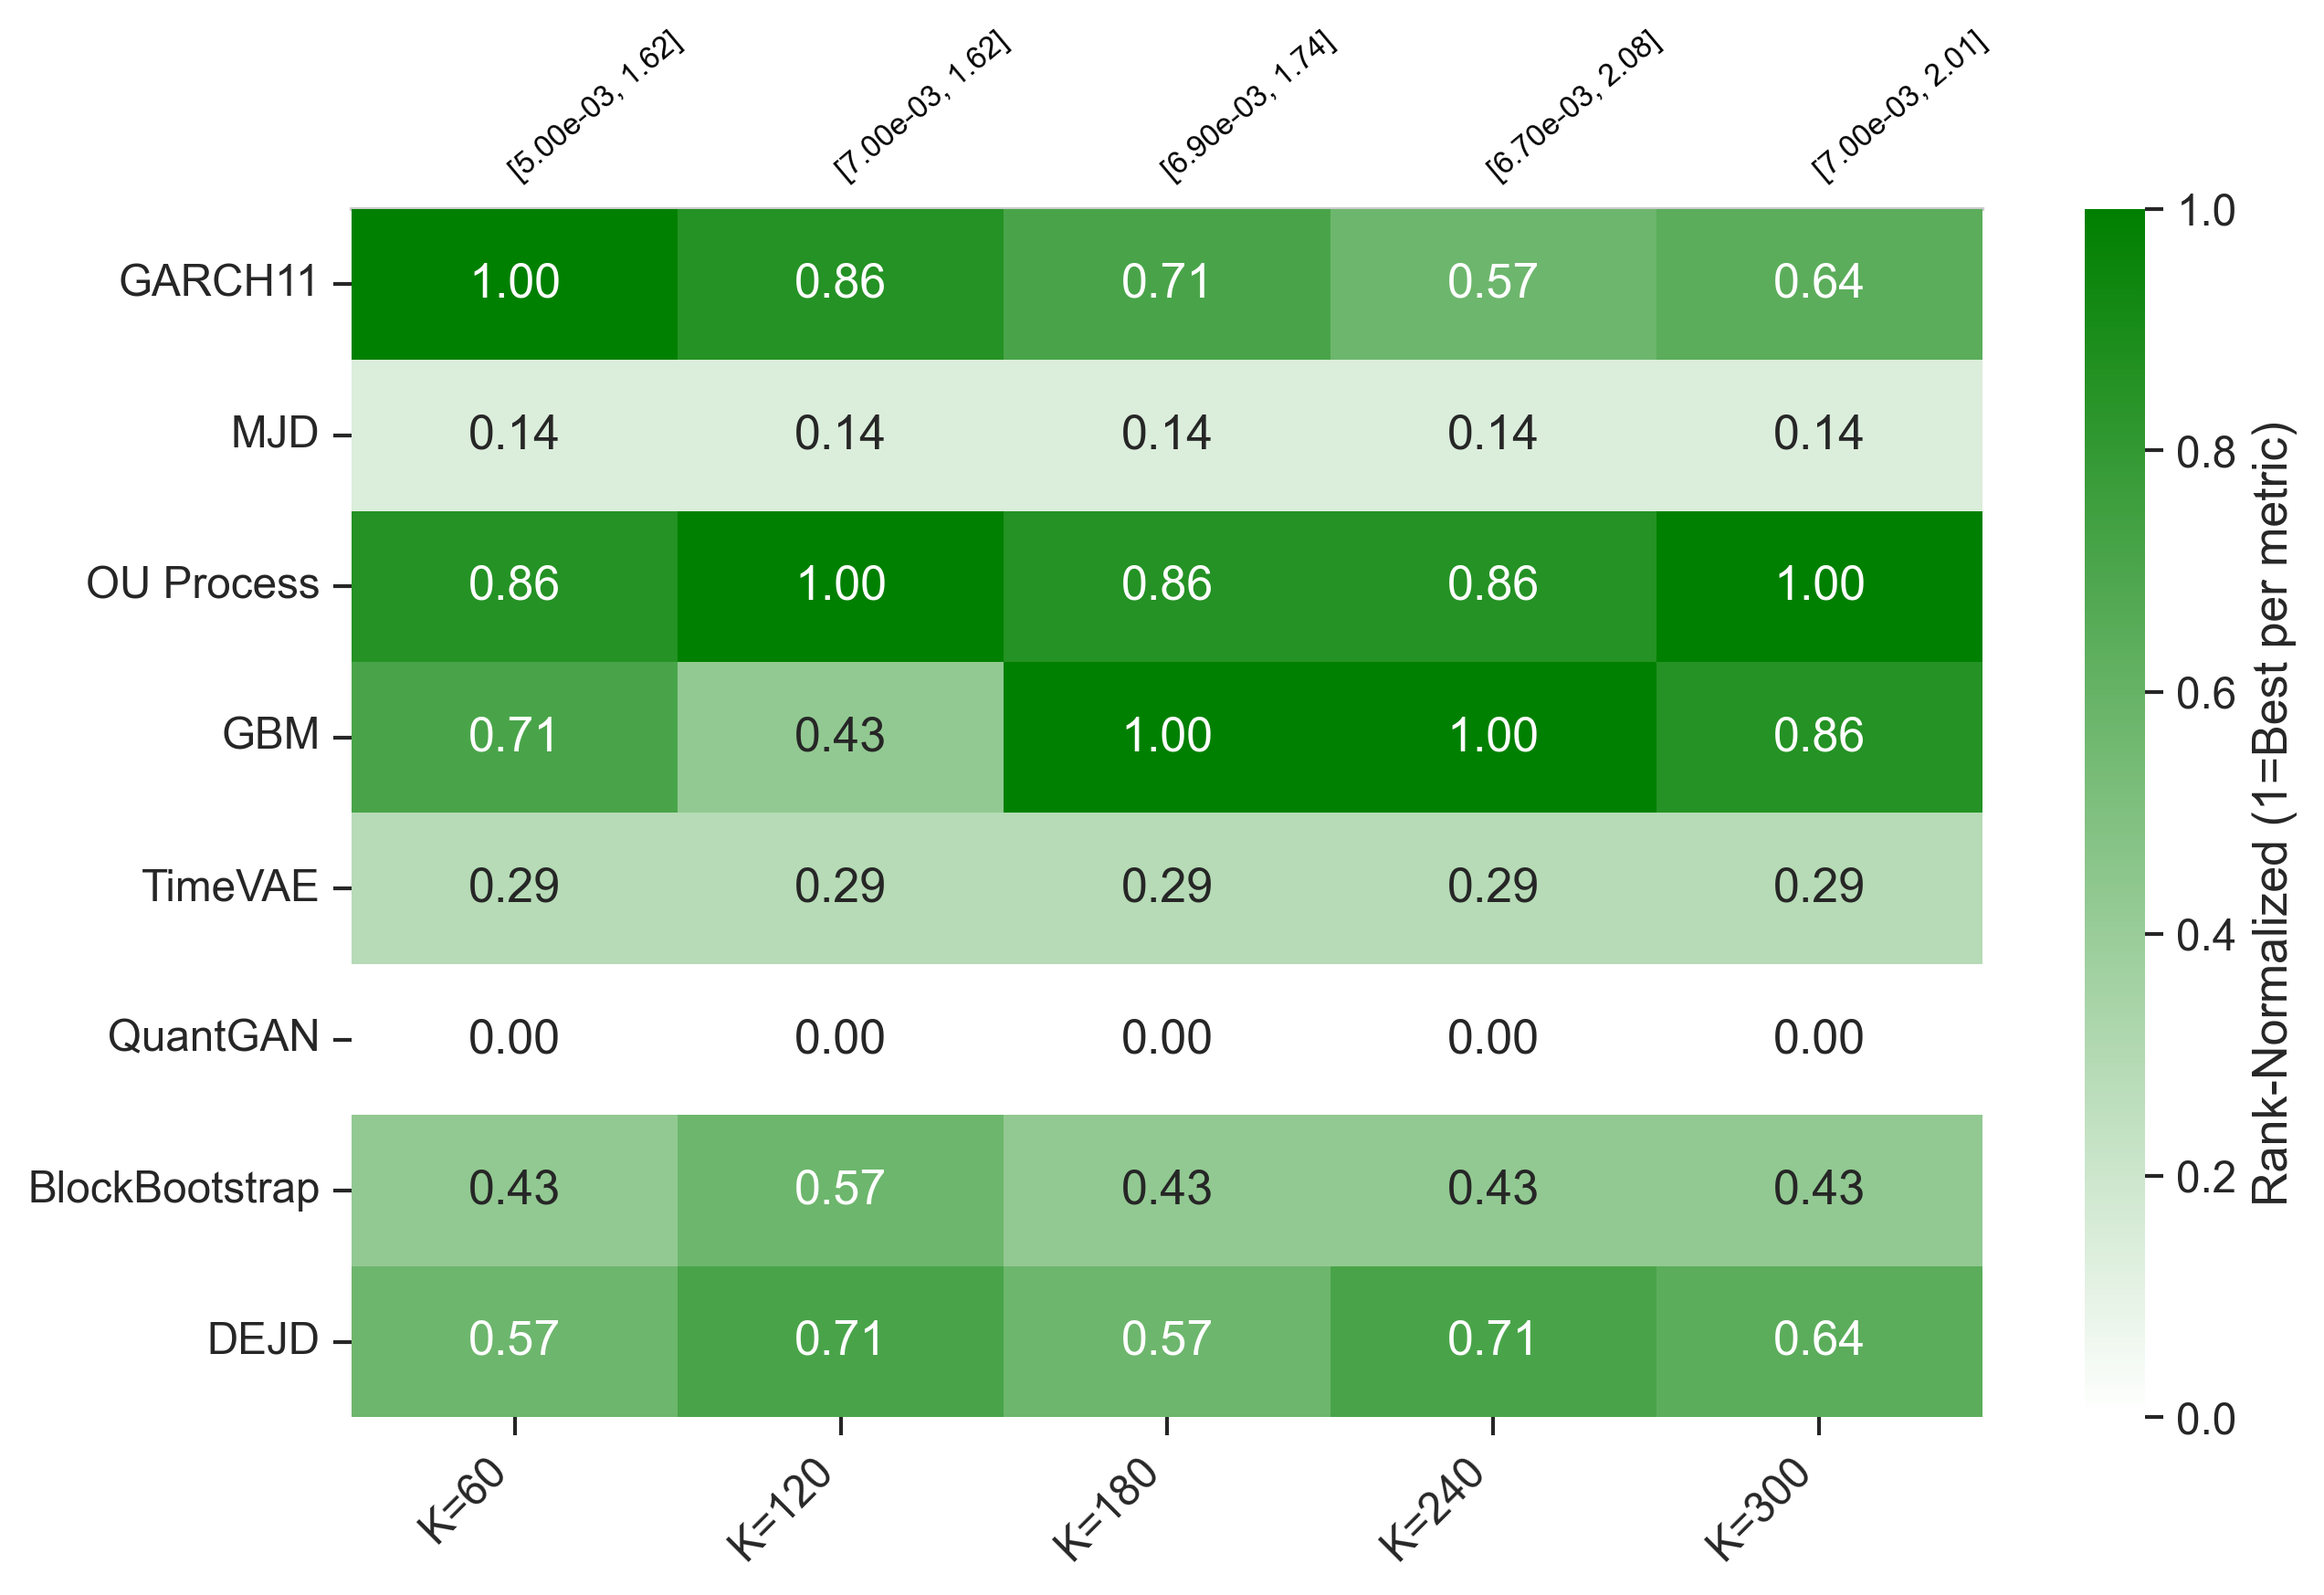
\includegraphics[width=0.9\textwidth,keepaspectratio]
  {../../results/ablation_studies/figure_3_metric_heatmaps_per_metric/figure_3_efficiency_per_metric_ranknorm.png}
  \caption{Ablation study: efficiency per-metric rank-normalized heatmap across sequence lengths.}
  \Description{Heatmap showing efficiency metrics across sequence length ablations.}
  \label{fig:ablation_efficiency}
\end{figure*}

\begin{figure*}[h]
  \centering
  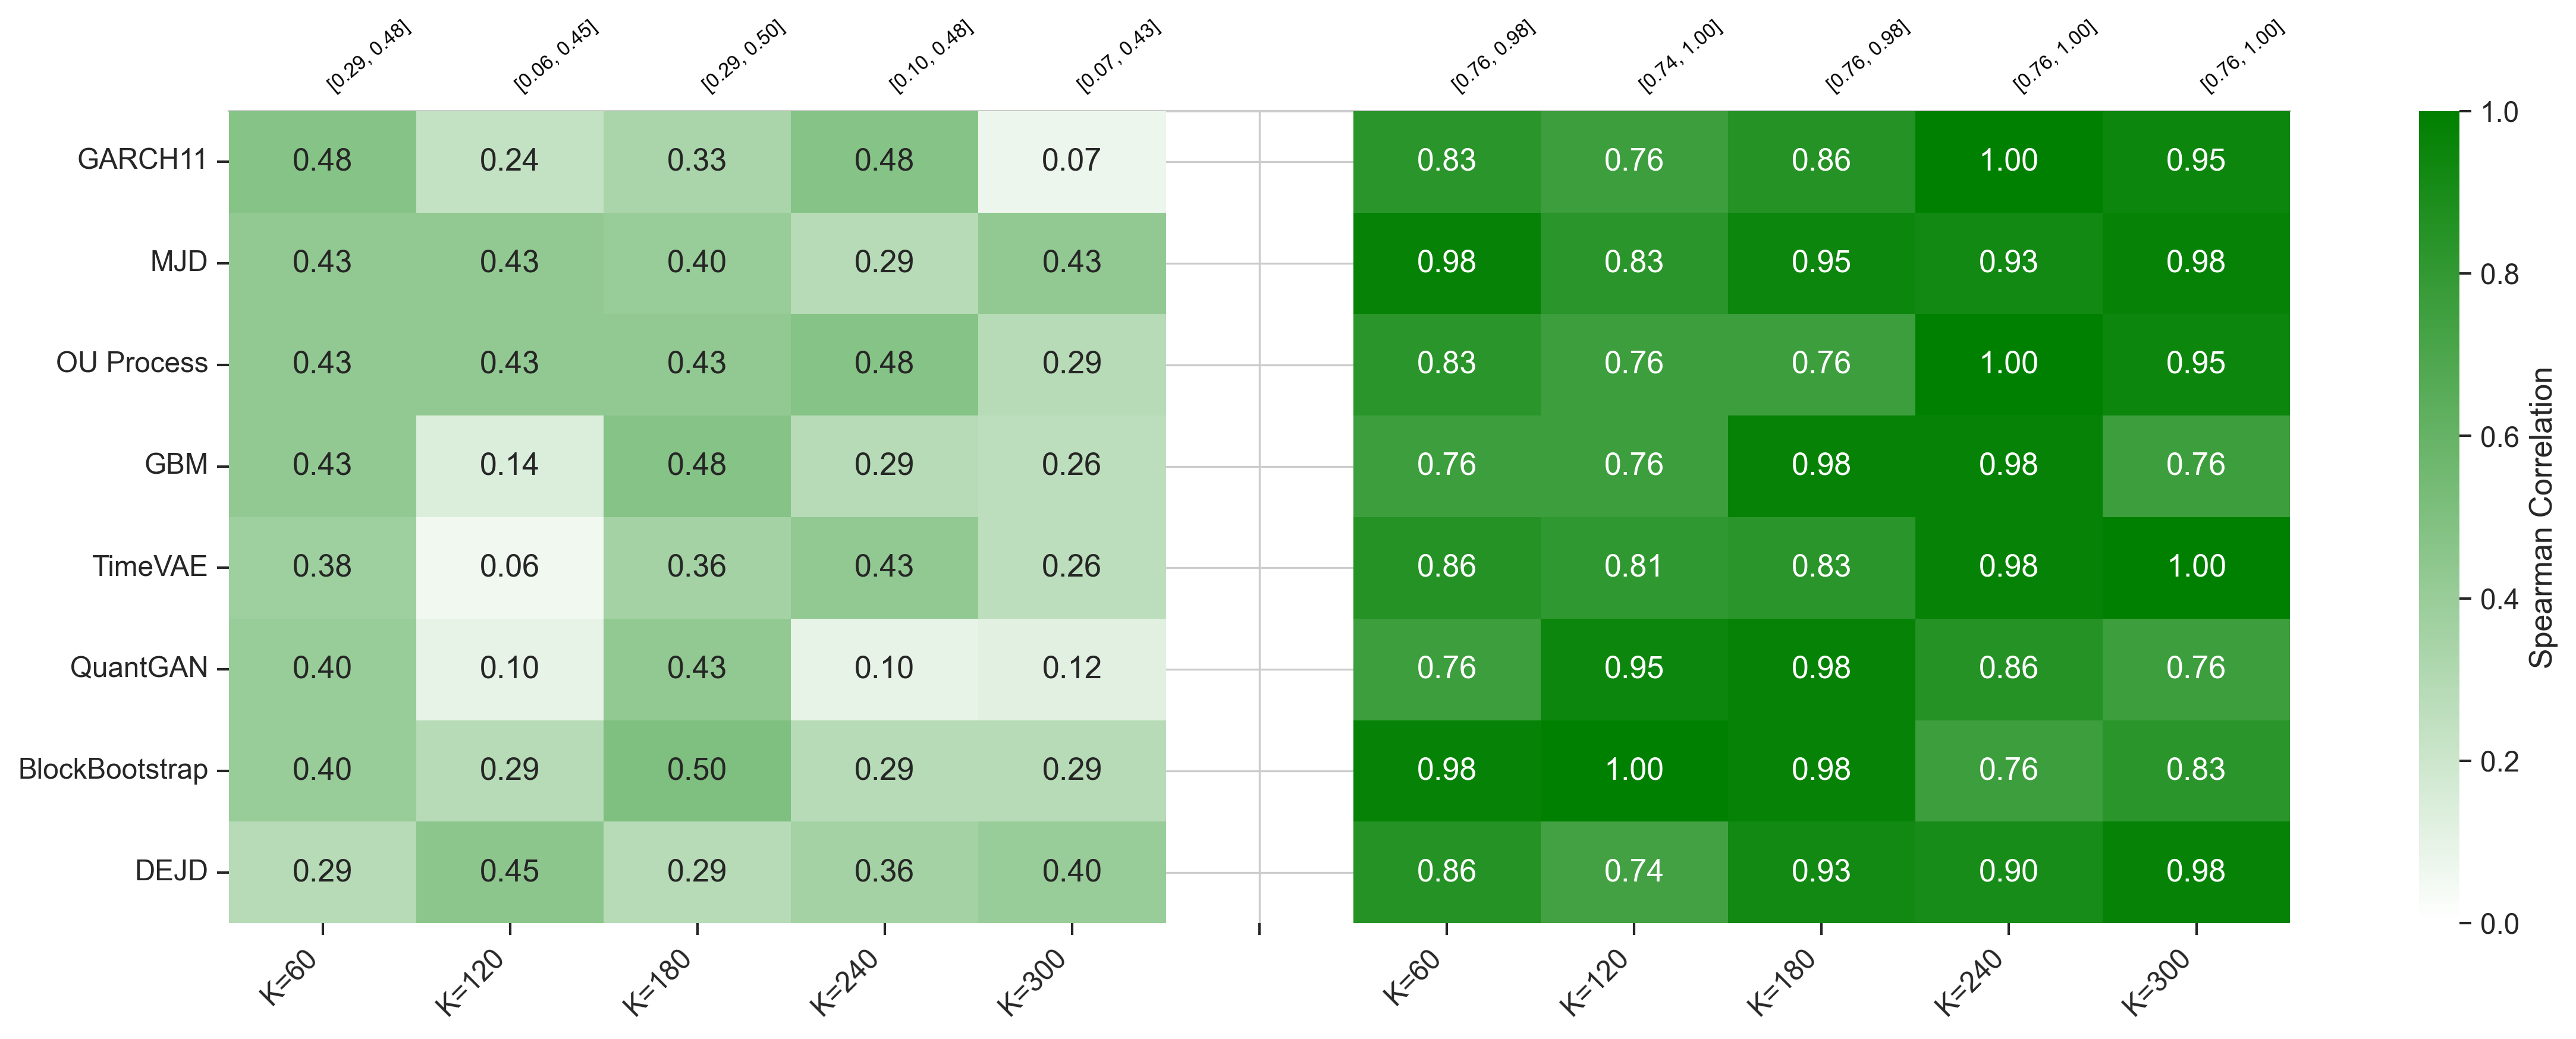
\includegraphics[width=0.9\textwidth,keepaspectratio]
  {../../results/ablation_studies/figure_3_metric_heatmaps_per_metric/figure_3_utility_spearman_and_mixed_per_seq.png}
  \caption{Ablation study: utility (Spearman) per-sequence-length comparison across hedger algorithms between real and sythetic data.}
  \Description{Heatmap or plot showing utility Spearman correlations per sequence length.}
  \label{fig:ablation_utility_spearman}
\end{figure*}

      \begin{figure*}[h]
      \centering
      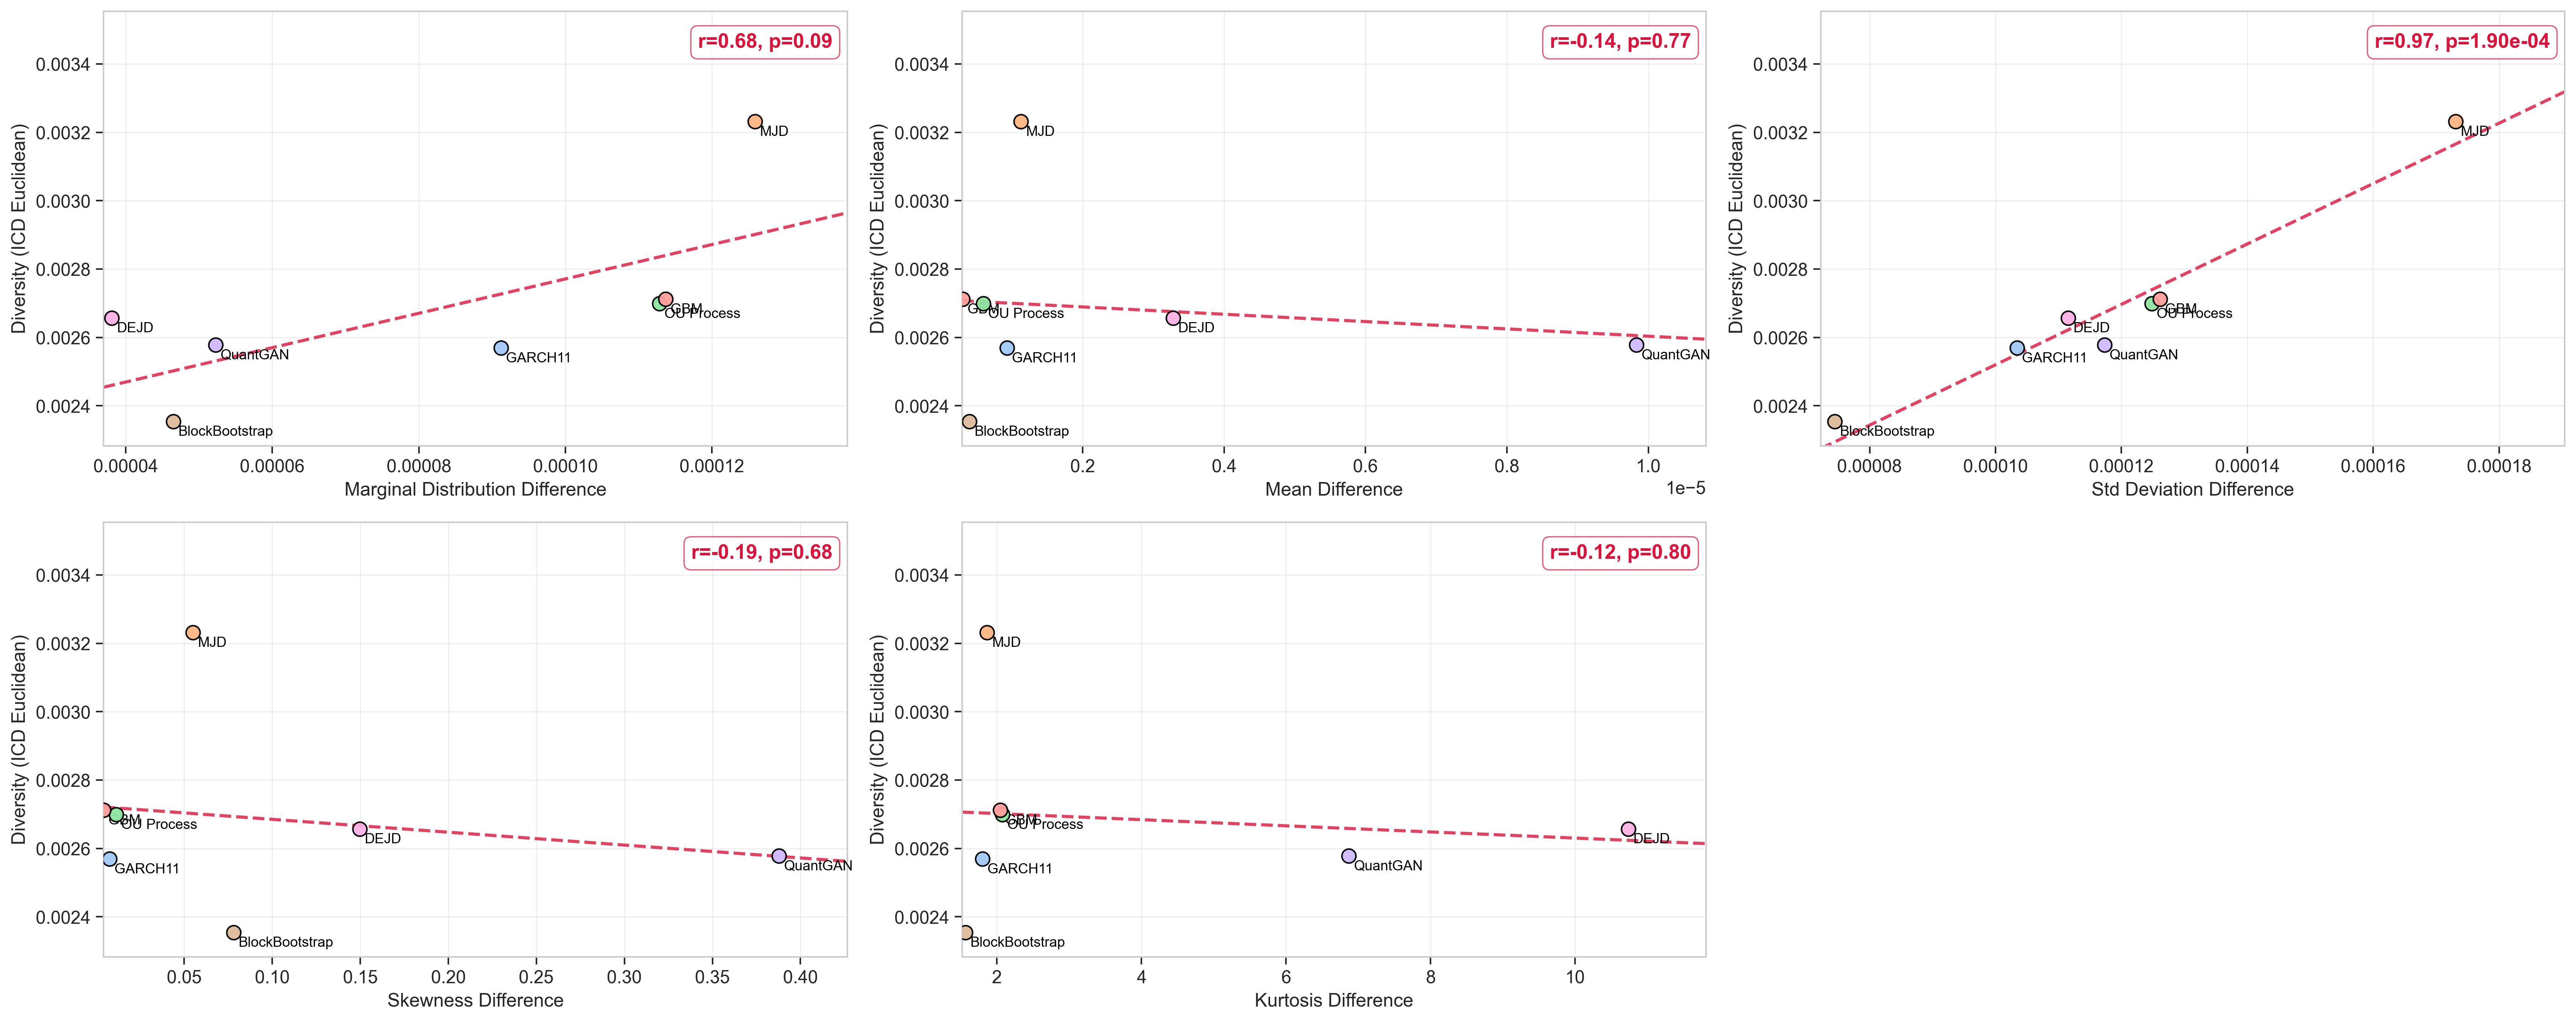
\includegraphics[width=\textwidth,height=10cm,keepaspectratio]
      {../../results/appendix/figure_5_fidelity_vs_diversity/figure_5_icd_euclidean_2x3_grid.png}
      \caption{Scatter plots and linear regression analysis showing the relationship between 
      fidelity metrics (MDD, MD, SDD, SD, KD, by row) and intra-class Euclidean distance (ICD-ED) 
      across all SDGFTS models. Each subplot displays the fitted regression line with 
      corresponding R² value and p-value, indicating the strength and statistical significance 
      of the linear relationship between fidelity and diversity.}
      \Description{A heatmap displaying the normalized rankings of diversity metrics for
      different SDGFTS models, highlighting the performance scores and their implications for model diversity.}
      \label{fig:eclidian_fidelity_diversity}
    \end{figure*}

      \begin{figure*}[h]
      \centering
      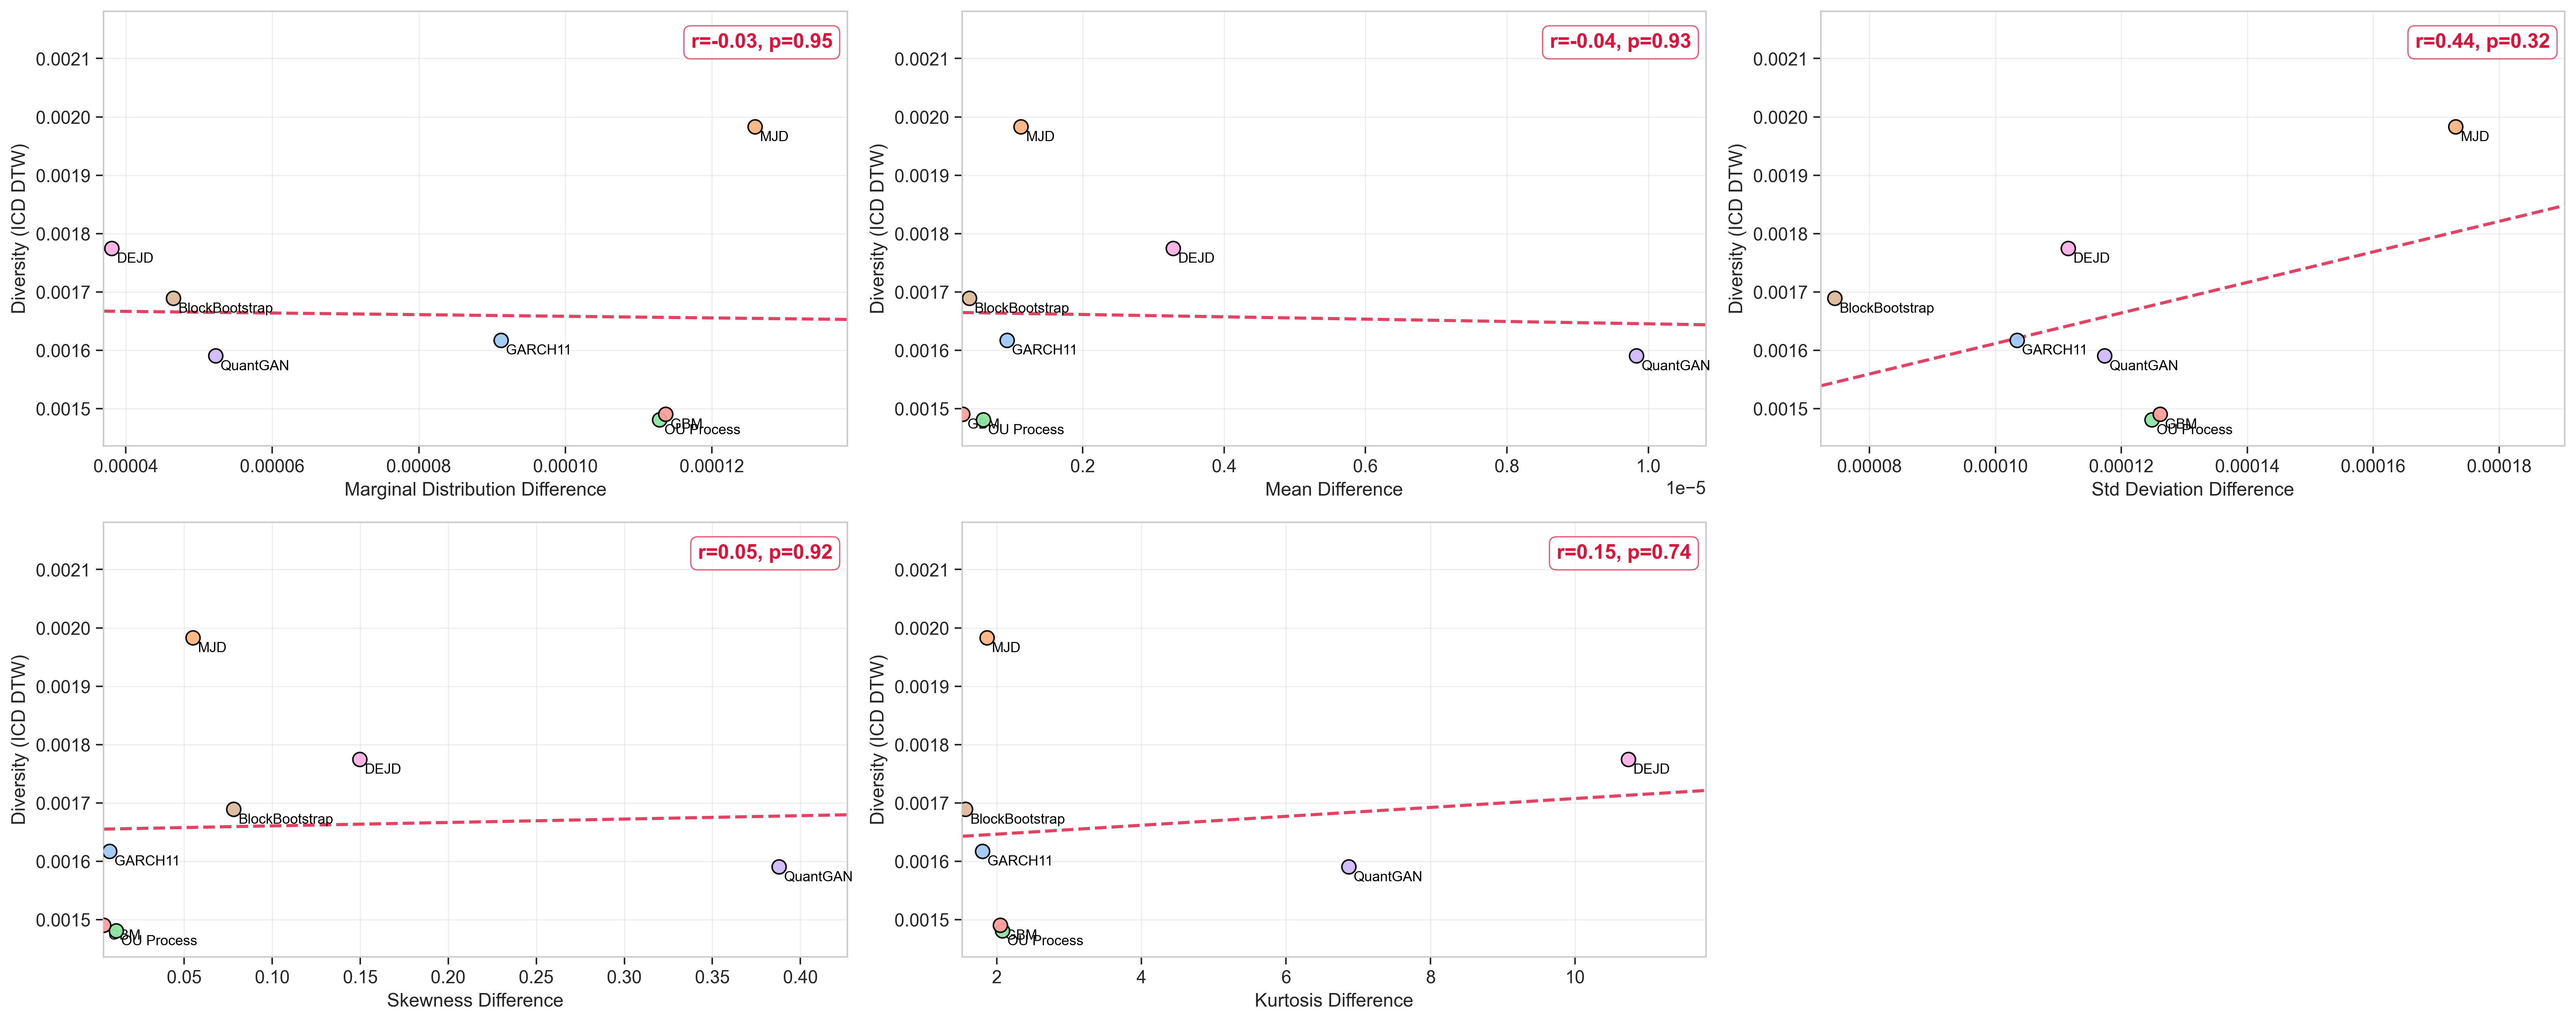
\includegraphics[width=\textwidth,height=10cm,keepaspectratio]
      {../../results/appendix/figure_5_fidelity_vs_diversity/figure_5_icd_dtw_2x3_grid.png}
      \caption{Scatter plots and linear regression analysis showing the relationship between 
      fidelity metrics (MDD, MD, SDD, SD, KD, by row) and intra-class DTW distance (ICD-DTW) 
      across all SDGFTS models. Each subplot displays the fitted regression line with 
      corresponding R² value and p-value, indicating the strength and statistical significance 
      of the linear relationship between fidelity and diversity measured by DTW.}
      \Description{Scatter plots showing the correlation between fidelity metrics and 
      ICD-DTW diversity across different SDGFTS models.}
      \label{fig:dtw_fidelity_diversity}
    \end{figure*}

      \begin{figure*}[h]
      \centering
      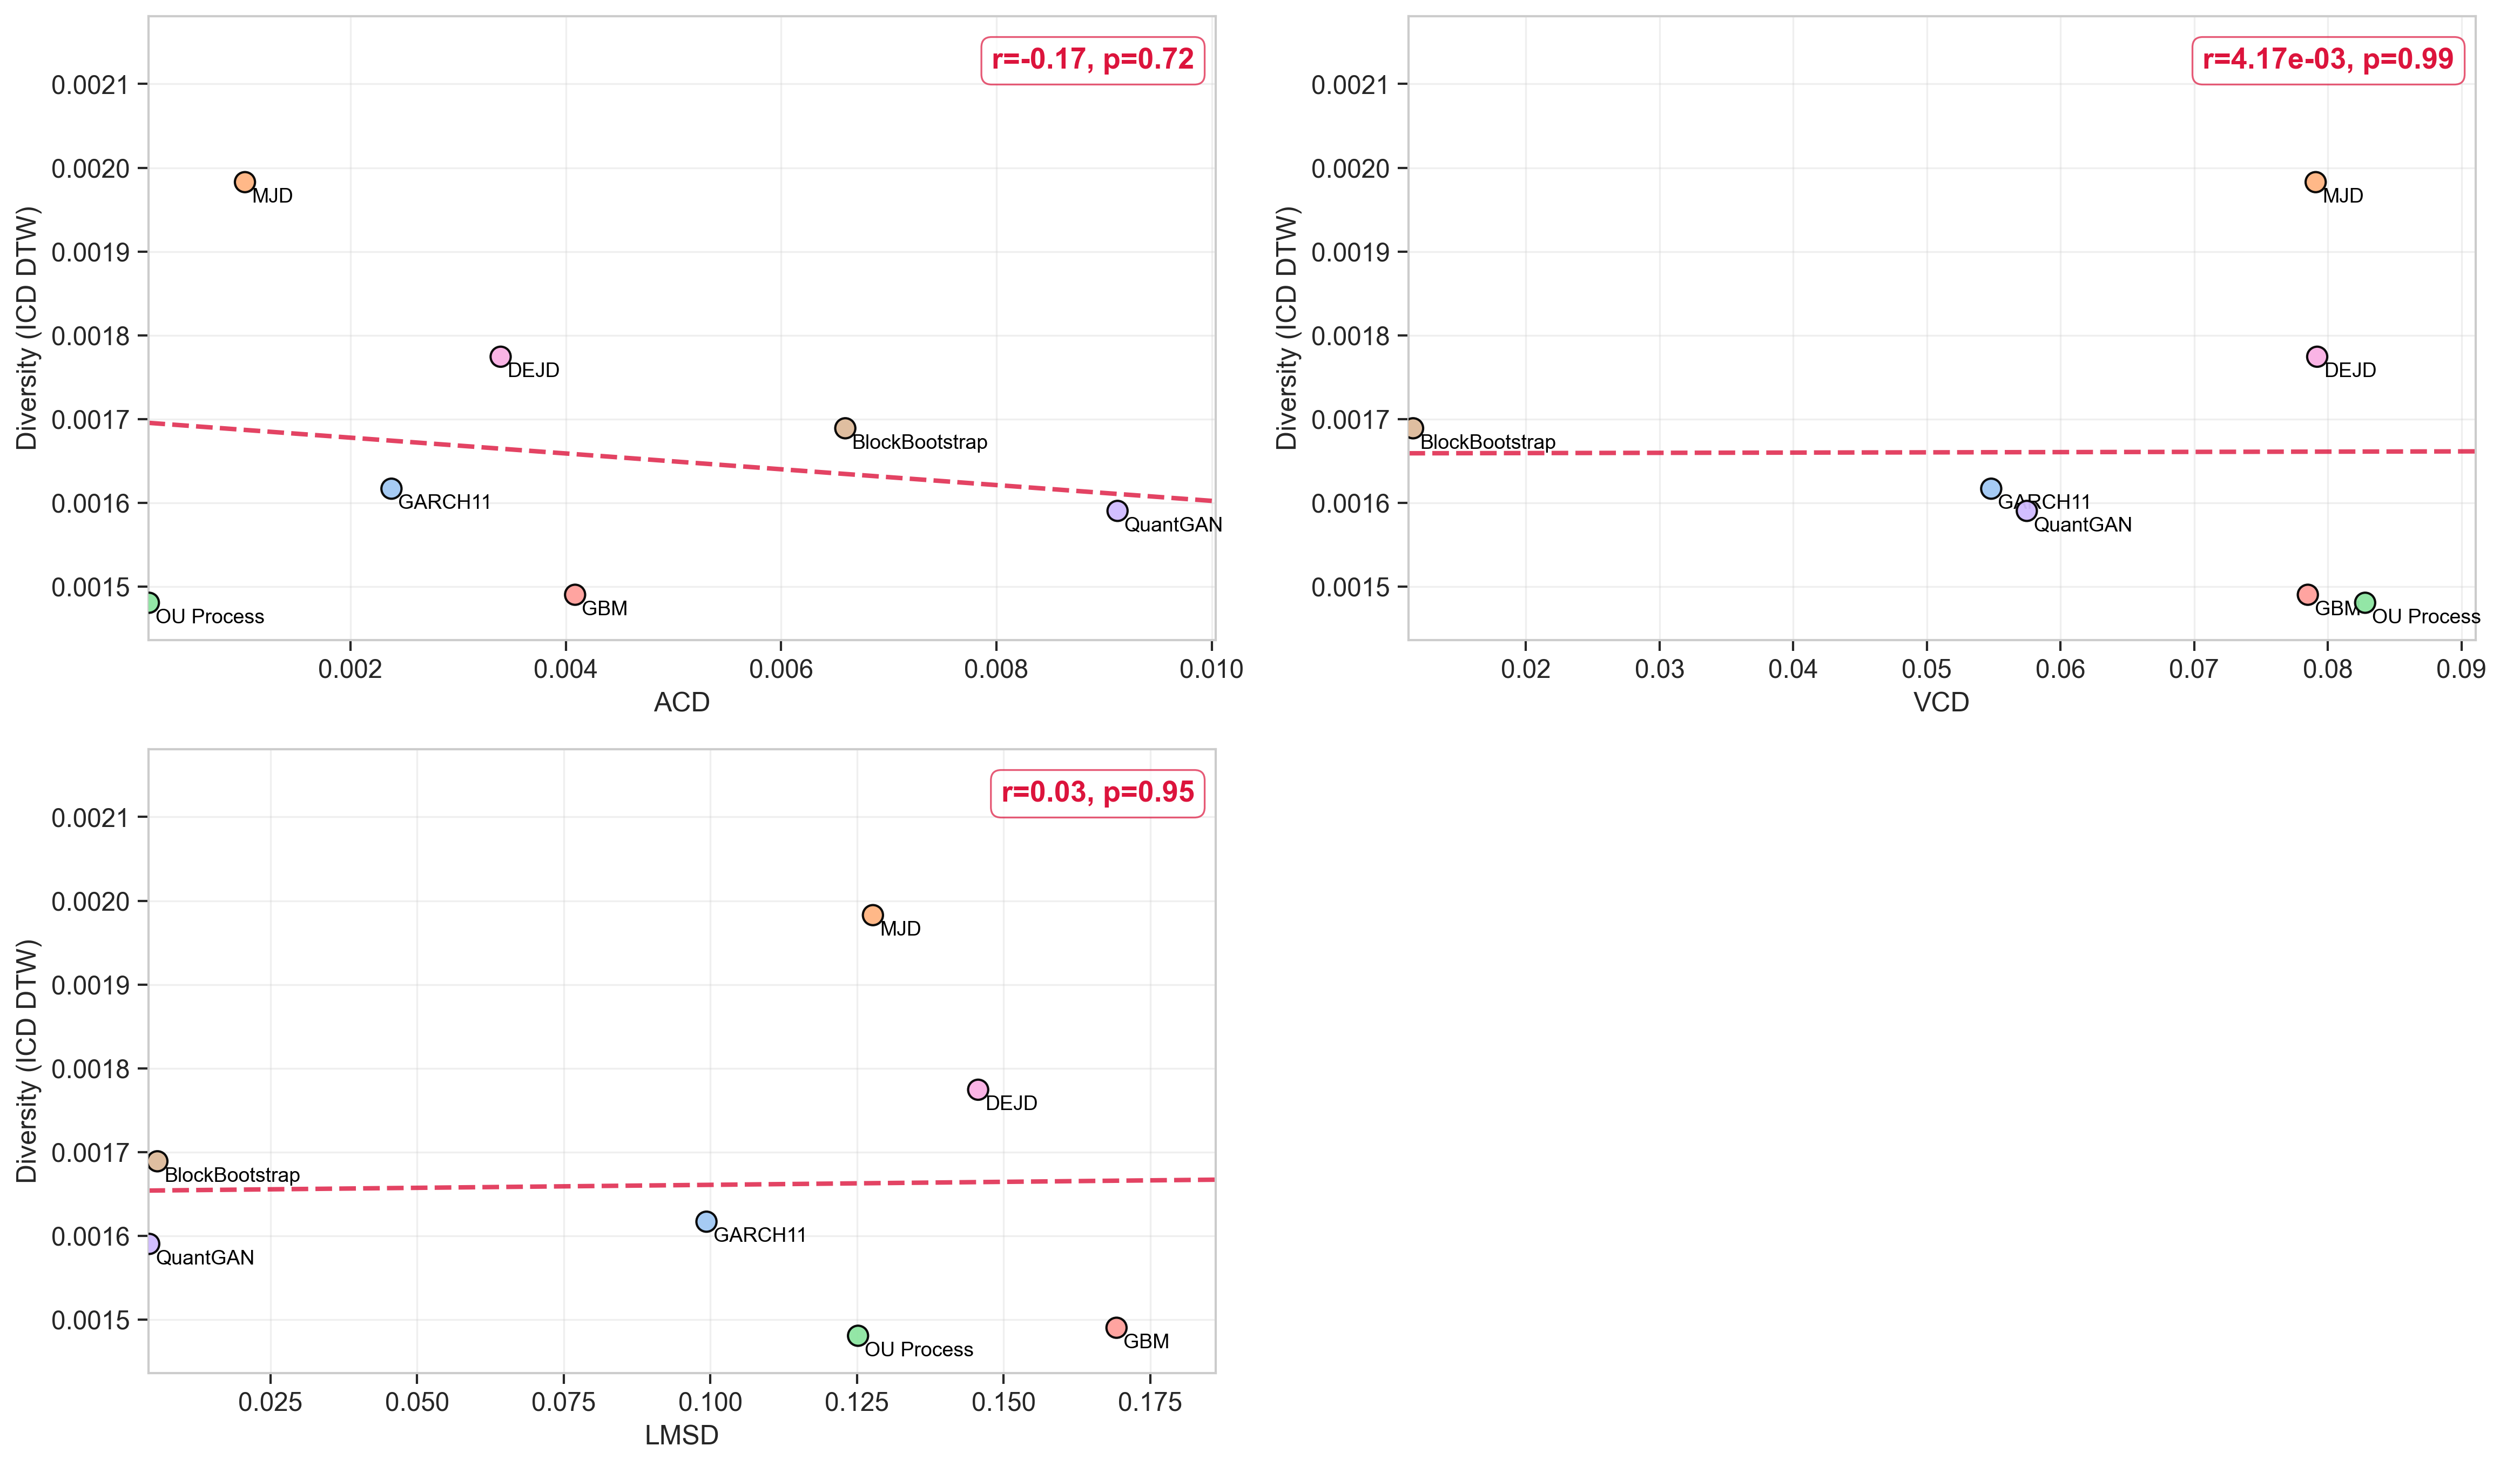
\includegraphics[width=\textwidth,height=10cm,keepaspectratio]
      {../../results/appendix/figure_6_stylized_facts_vs_diversity/figure_6_icd_dtw_2x2_grid.png}
      \caption{Scatter plots showing the relationship between stylized facts metrics 
      (ACD, volatility clustering, and LMSD) and intra-class DTW distance (ICD-DTW) 
      across all SDGFTS models. Each point represents a model, with trend lines 
      indicating correlation direction and strength.}
      \Description{Scatter plots illustrating the correlation between stylized facts 
      metrics and ICD-DTW diversity across different models.}
      \label{fig:dtw_stylized_facts_diversity}
    \end{figure*}

\section{Supplementary t-SNE Visualizations}

\begin{figure*}[h]
  \centering
  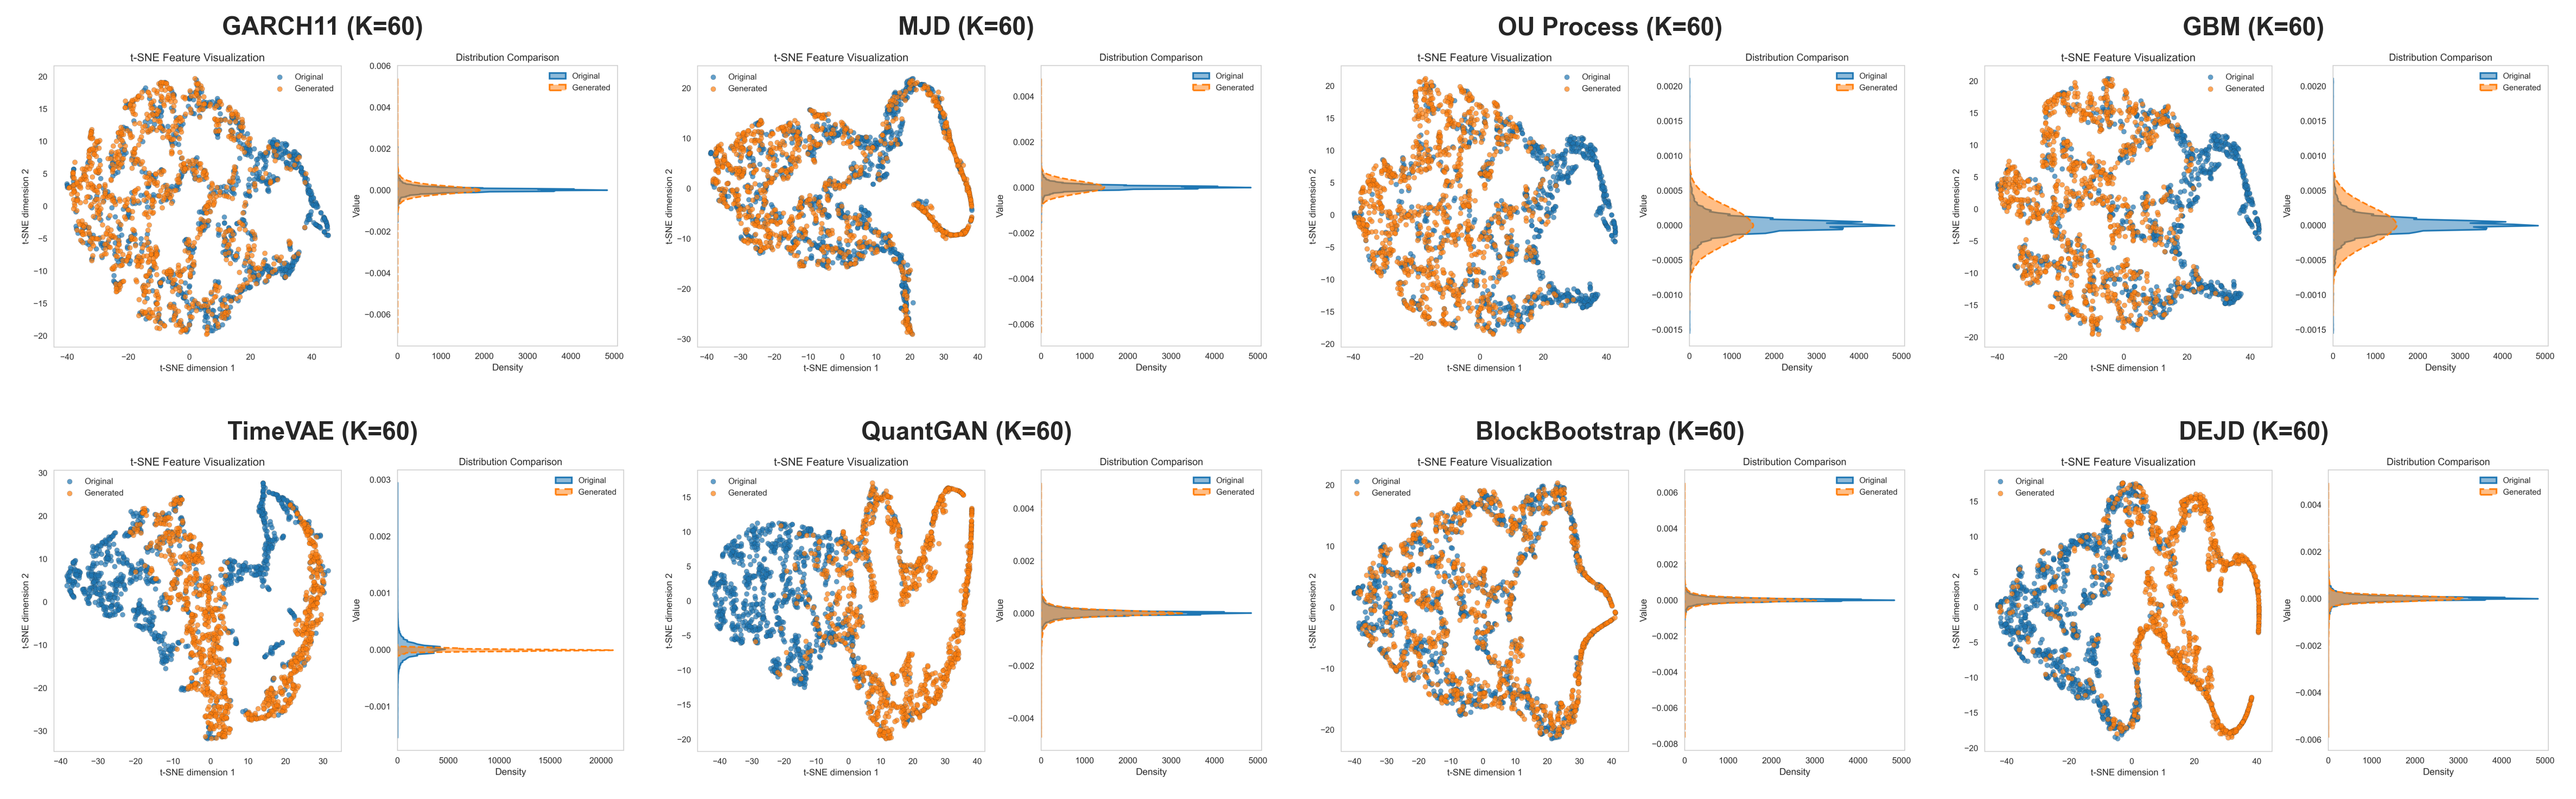
\includegraphics[width=0.9\textwidth,keepaspectratio]
  {../../results/appendix/figure_4_tsne_supplementary/figure_4_seq_60.png}
  \caption{Supplementary t-SNE visualization for sequence length 60 minutes.}
  \Description{t-SNE embeddings comparing real and synthetic data for 60-minute sequences.}
  \label{fig:tsne_seq_60}
\end{figure*}

\begin{figure*}[h]
  \centering
  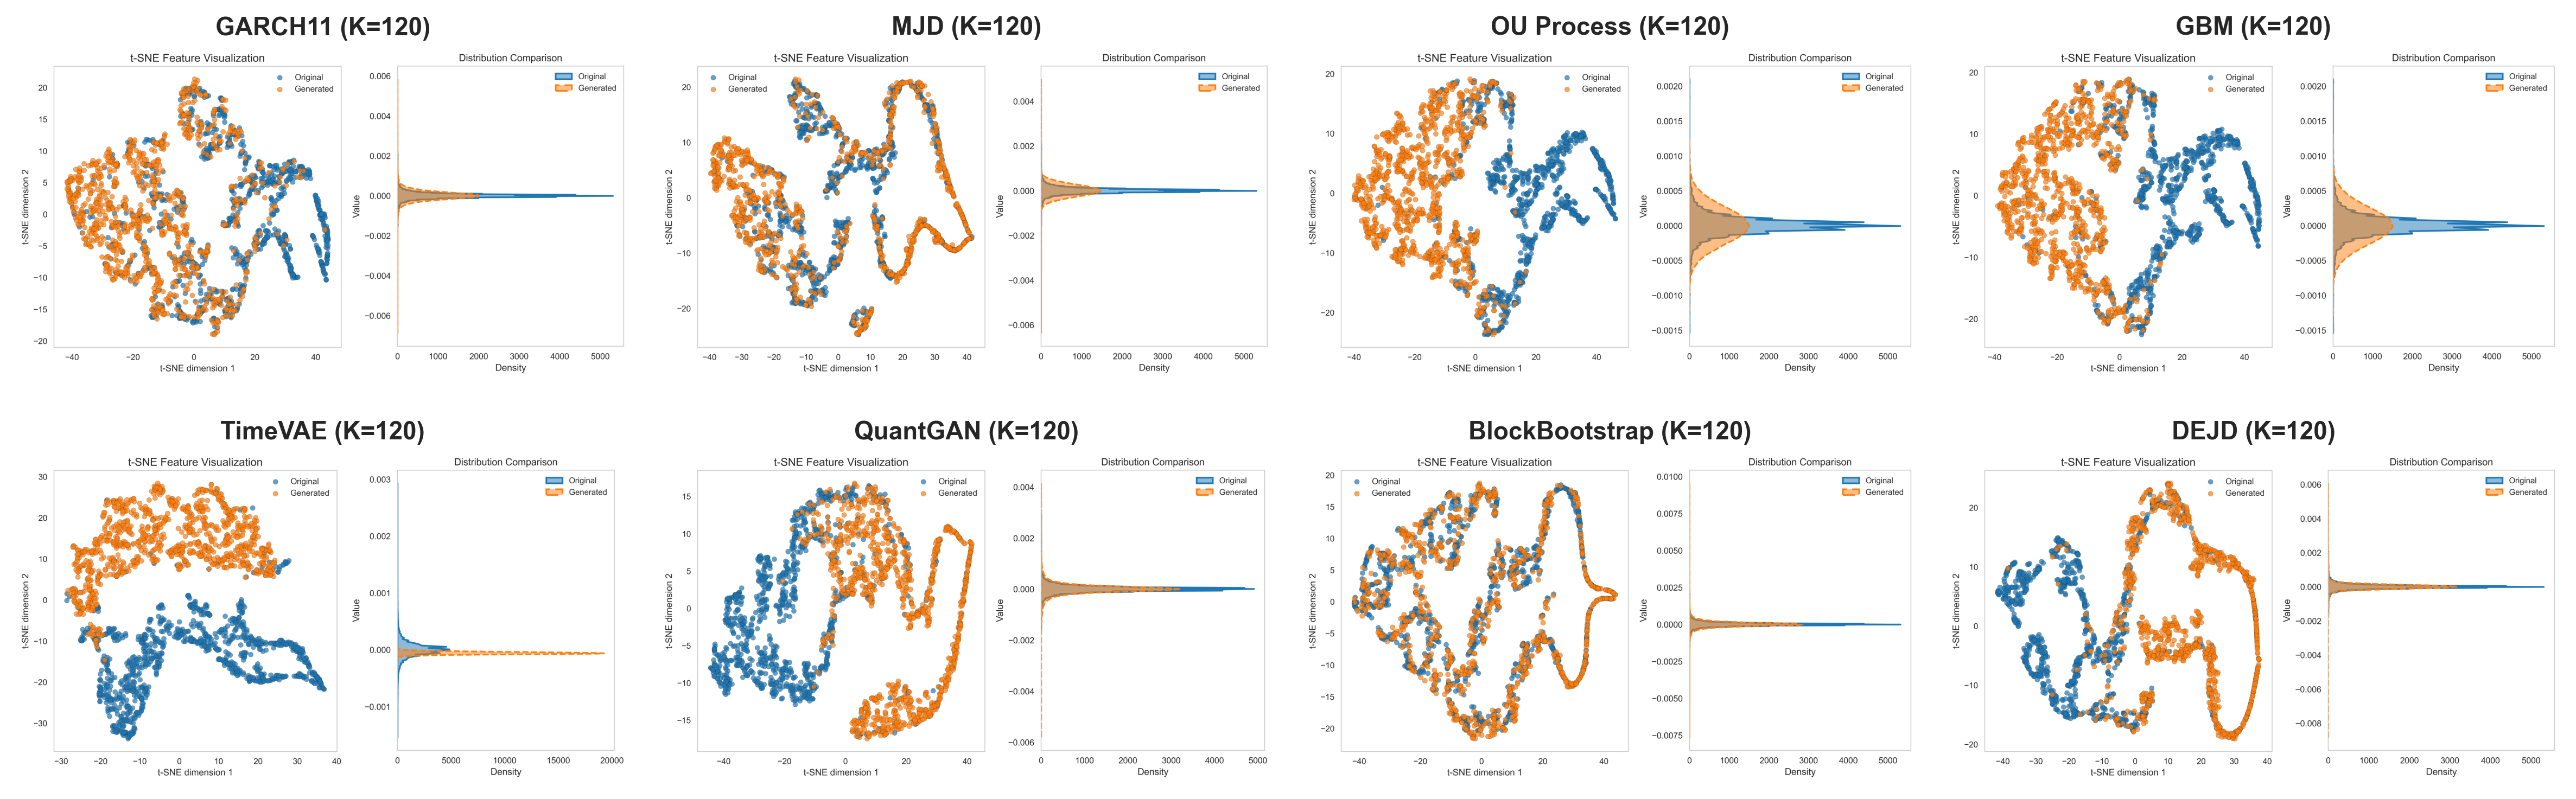
\includegraphics[width=0.9\textwidth,keepaspectratio]
  {../../results/appendix/figure_4_tsne_supplementary/figure_4_seq_120.png}
  \caption{Supplementary t-SNE visualization for sequence length 120 minutes.}
  \Description{t-SNE embeddings comparing real and synthetic data for 120-minute sequences.}
  \label{fig:tsne_seq_120}
\end{figure*}

\begin{figure*}[h]
  \centering
  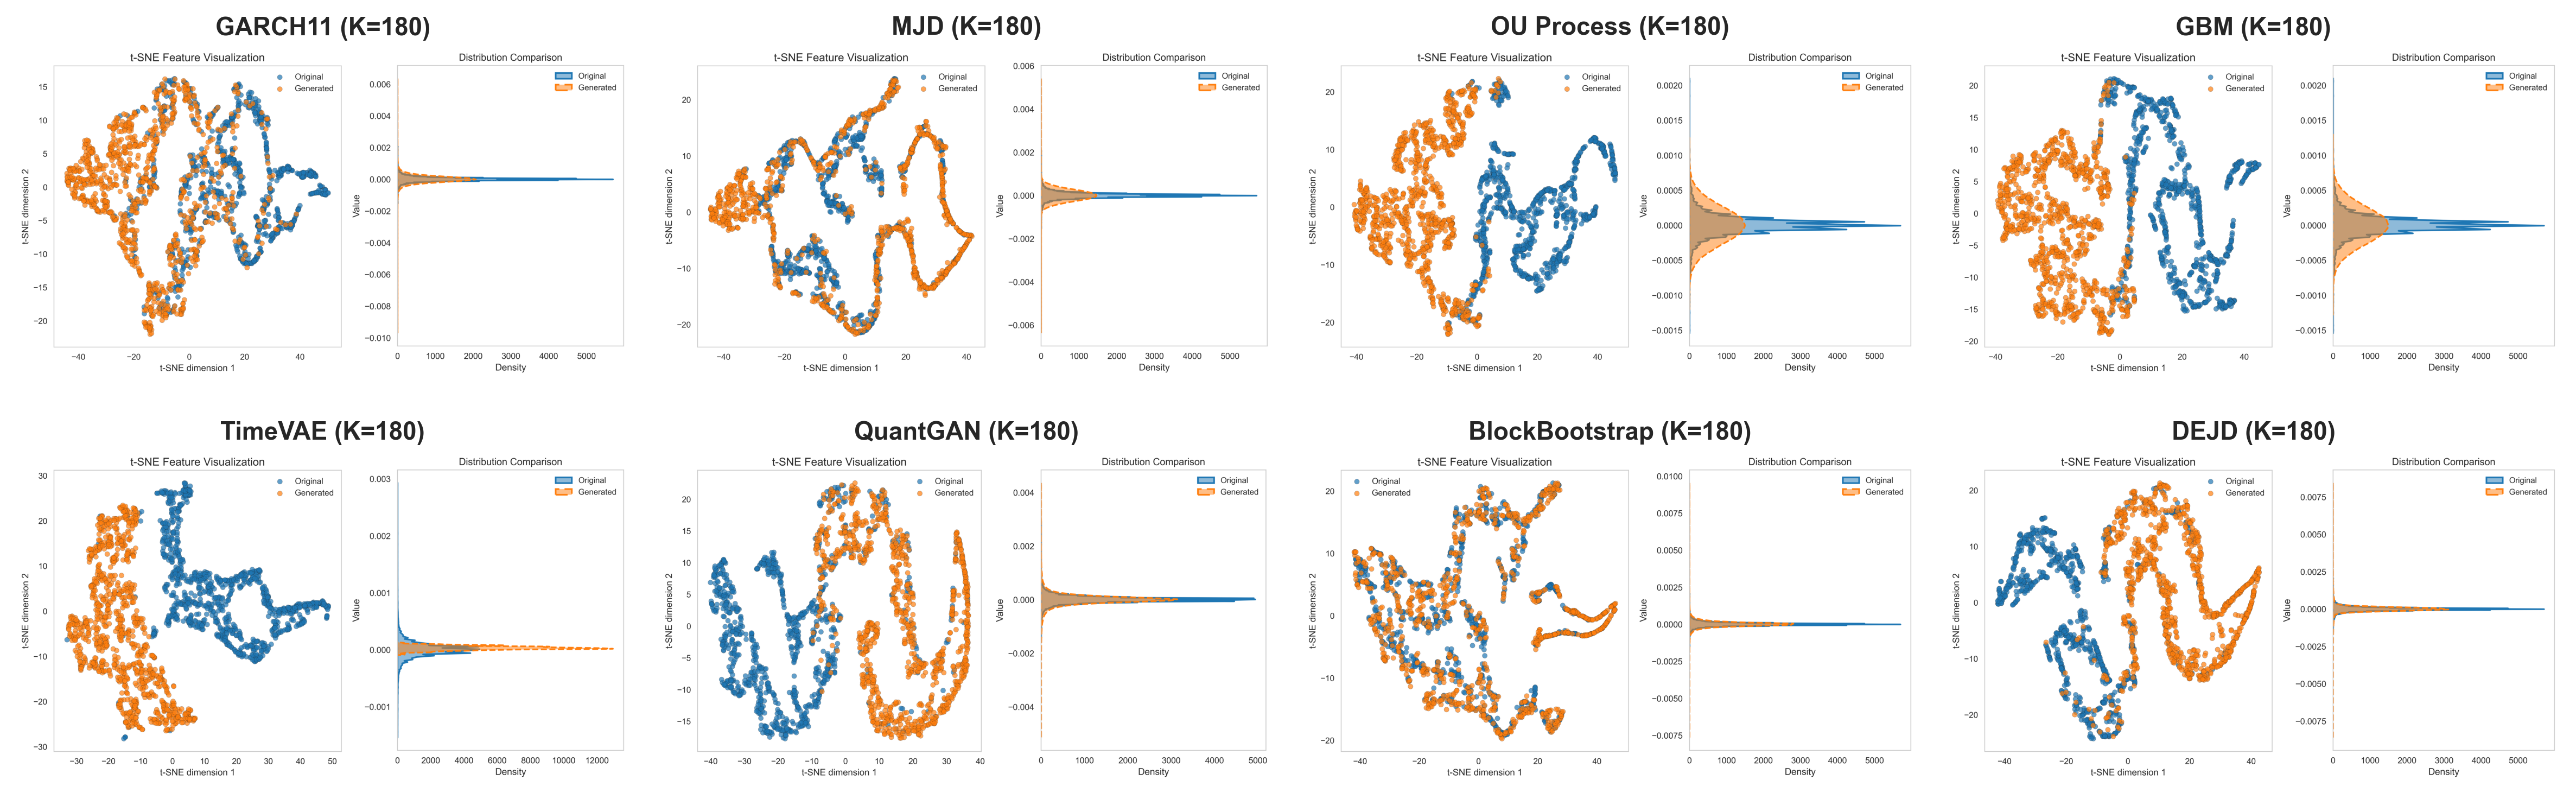
\includegraphics[width=0.9\textwidth,keepaspectratio]
  {../../results/appendix/figure_4_tsne_supplementary/figure_4_seq_180.png}
  \caption{Supplementary t-SNE visualization for sequence length 180 minutes.}
  \Description{t-SNE embeddings comparing real and synthetic data for 180-minute sequences.}
  \label{fig:tsne_seq_180}
\end{figure*}

\begin{figure*}[h]
  \centering
  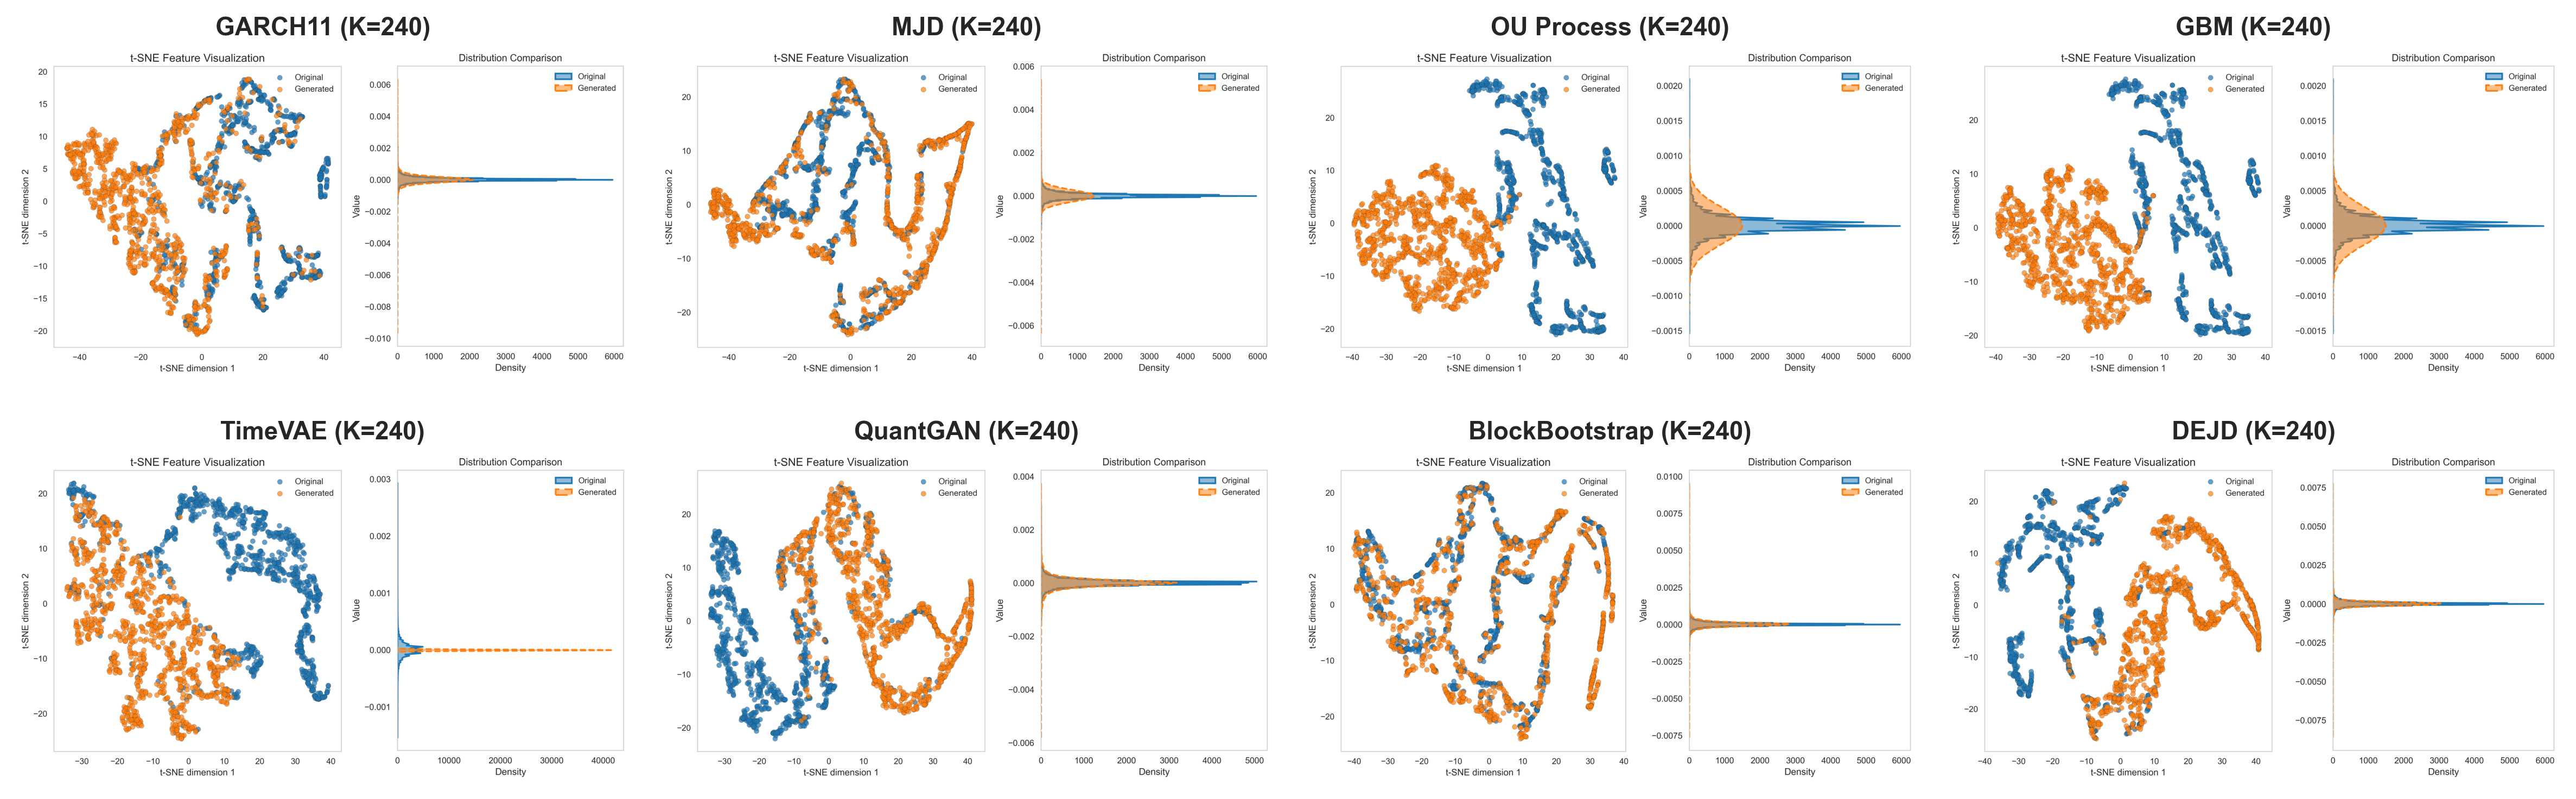
\includegraphics[width=0.9\textwidth,keepaspectratio]
  {../../results/appendix/figure_4_tsne_supplementary/figure_4_seq_240.png}
  \caption{Supplementary t-SNE visualization for sequence length 240 minutes.}
  \Description{t-SNE embeddings comparing real and synthetic data for 240-minute sequences.}
  \label{fig:tsne_seq_240}
\end{figure*}

\begin{figure*}[h]
  \centering
  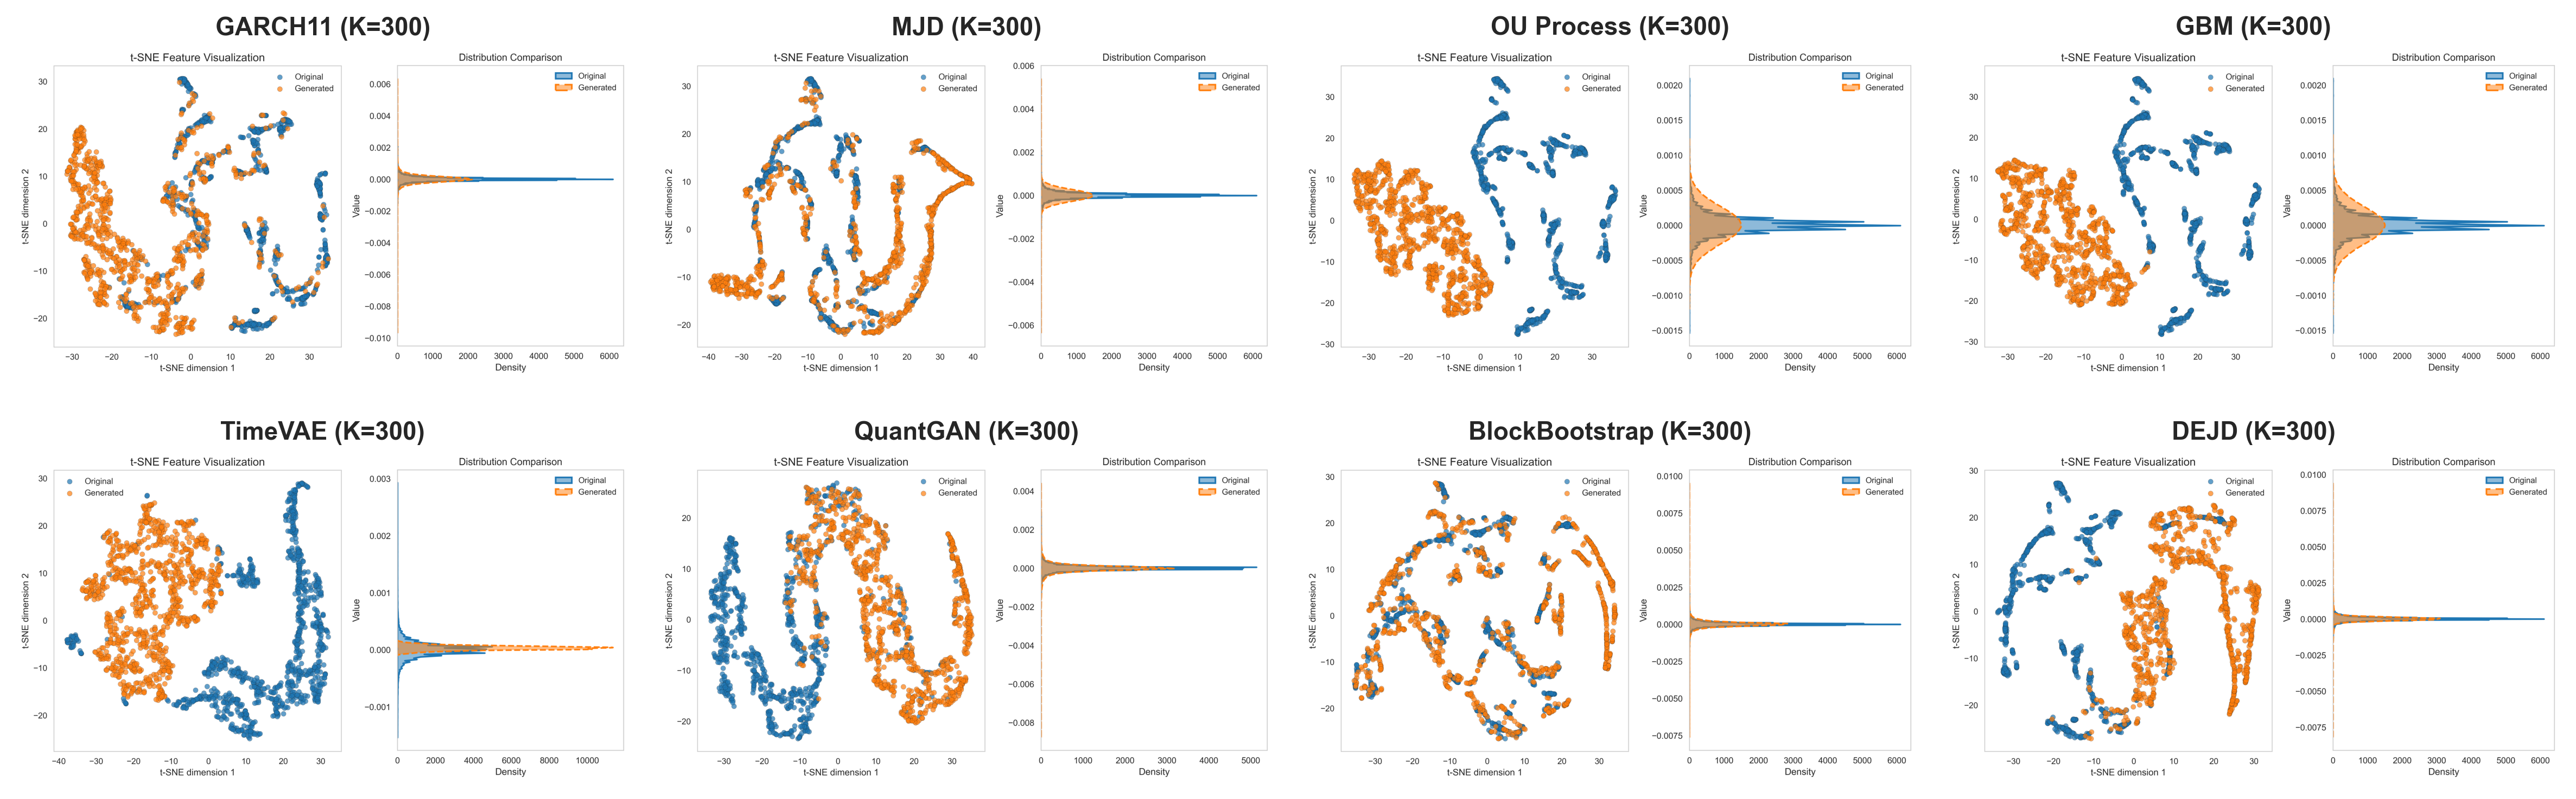
\includegraphics[width=0.9\textwidth,keepaspectratio]
  {../../results/appendix/figure_4_tsne_supplementary/figure_4_seq_300.png}
  \caption{Supplementary t-SNE visualization for sequence length 300 minutes.}
  \Description{t-SNE embeddings comparing real and synthetic data for 300-minute sequences.}
  \label{fig:tsne_seq_300}
\end{figure*}

\section{Augmented Testing Analysis}

\begin{figure*}[h]
  \centering
  
\includegraphics[width=\textwidth,keepaspectratio]
  {../../results/appendix/figure_7_augmented_testing_delta/figure_7_augmented_testing_2x4_delta.png}
  \caption{Augmented testing performance comparison showing delta metrics 
  across different hedger algorithms and SDGFTS models. Each subplot compares 
  performance when training on real data only versus augmented data 
  (real + synthetic).}
  \Description{Grid of plots showing augmented testing delta metrics for 
  different hedger models and synthetic data generators.}
  \label{fig:augmented_testing_delta}
\end{figure*}




\end{document}
